\documentclass[a4paper]{scrartcl}

\usepackage[
fancytheorems,
fancyproofs,
noindent
]{adam}

\usepackage{tikz}
\usepackage{bbm}
\usepackage{mathtools}

\usetikzlibrary{positioning, arrows.meta, calc}

\title{Probability and Measure}
\author{Adam Kelly (\texttt{ak2316@cam.ac.uk})}
\date{\today}

% Extra macros for this course
\newcommand{\cA}{\mathcal{A}}
\newcommand{\cB}{\mathcal{B}}
\newcommand{\cC}{\mathcal{C}}
\newcommand{\cD}{\mathcal{D}}
\newcommand{\cE}{\mathcal{E}}
\newcommand{\cF}{\mathcal{F}}
\newcommand{\cG}{\mathcal{G}}
\newcommand{\cH}{\mathcal{H}}
\newcommand{\cI}{\mathcal{I}}
\newcommand{\cL}{\mathcal{L}}
\newcommand{\cM}{\mathcal{M}}
\newcommand{\cN}{\mathcal{N}}
\newcommand{\cT}{\mathcal{T}}
\newcommand{\cV}{\mathcal{V}}
\newcommand{\cX}{\mathcal{X}}
\newcommand{\cY}{\mathcal{Y}}
\newcommand{\ip}[2]{\langle #1, #2 \rangle}
\DeclareMathOperator*{\esssup}{ess\,sup}
\newcommand{\ind}{\ii}
\newcommand{\weakto}{\xrightarrow{\;w\;}}

\allowdisplaybreaks

\begin{document}

\maketitle

Measure theory is the machinery that makes `size' -- length, area, volume, probability -- into something we can actually do analysis with. The Riemann integral of Analysis I is a perfectly serviceable tool for integrating continuous functions on a closed interval, but it is fragile: it does not interact well with limits, the space of Riemann integrable functions is not complete, and it has nothing whatsoever to say about integration over abstract spaces. Lebesgue's insight was that if one is willing to work harder at the front end -- assigning a measure to sets before integrating functions -- then the integral one gets at the back end is enormously more robust.

Probability theory is where this pays off most spectacularly. Kolmogorov's observation, in 1933, was that a probability is nothing more than a measure of total mass one, a random variable is nothing more than a measurable function, and an expectation is nothing more than an integral. Once one accepts this dictionary, the great limit theorems of probability -- the strong law of large numbers, the central limit theorem -- become theorems about the convergence of integrals, and the tools of measure theory apply directly. In this course we will build the theory from the ground up and then spend the second half cashing it in.

This article constitutes my notes for the `Probability and Measure' course, held in Michaelmas 2022 at Cambridge. These notes are \emph{not a transcription of the lectures}, and differ significantly in quite a few areas. Still, all lectured material should be covered.

\tableofcontents

\section{Introduction}

Let us begin by seeing what goes wrong with the integral we already have, because the shape of the fix is visible in the shape of the failure.

Recall from Analysis I that a bounded function $f : [a,b] \to \R$ is Riemann integrable if the supremum of the lower sums equals the infimum of the upper sums, where the sums are taken over partitions of $[a,b]$ into finitely many intervals. The essential move is to \emph{chop up the domain} into small intervals and, on each one, to pretend that $f$ is constant. That is a good idea when $f$ is continuous, since then $f$ really is nearly constant on small intervals. It is a terrible idea otherwise.

\begin{example}[The indicator of the rationals]
	Let $f = \ind_{\Q \cap [0,1]}$, so $f(x) = 1$ if $x$ is rational and $0$ otherwise. On every subinterval of $[0,1]$, however small, $f$ takes both the value $0$ and the value $1$. So every lower sum is $0$ and every upper sum is $1$, and $f$ is not Riemann integrable.

	But morally the answer ought to be $0$: the rationals are a countable set, they are `negligible' in $[0,1]$, and $f$ is zero off a negligible set. The Riemann integral has no way to express this thought.
\end{example}

The deeper problem is that the Riemann integral behaves badly under limits. Enumerate $\Q \cap [0,1]$ as $q_1, q_2, \dots$ and let $f_n = \ind_{\{q_1,\dots,q_n\}}$. Each $f_n$ is Riemann integrable with integral $0$, and $f_n \uparrow f$ pointwise, and yet the limit is not integrable at all. Any theorem of the form `if $f_n \to f$ then $\int f_n \to \int f$' must, for the Riemann integral, carry hypotheses strong enough (uniform convergence, say) to rule out most of the situations one actually meets.

Lebesgue's alternative is to \emph{chop up the range} instead. If $f \geq 0$, then instead of asking `how much does $f$ vary on $[x_i, x_{i+1}]$?' we ask `how big is the set on which $f$ exceeds $y$?'. Writing $\mu$ for `size', we would like to say something like
$$
\int f \approx \sum_j y_j \, \mu\big( \{ x : y_j \leq f(x) < y_{j+1} \} \big),
$$
approximating $f$ from below by functions taking finitely many values. The point is that the sets $\{y_j \leq f < y_{j+1}\}$ are allowed to be horrible -- they need not be intervals, or finite unions of intervals, or anything one can draw -- provided only that we can assign them a size.

\begin{center}
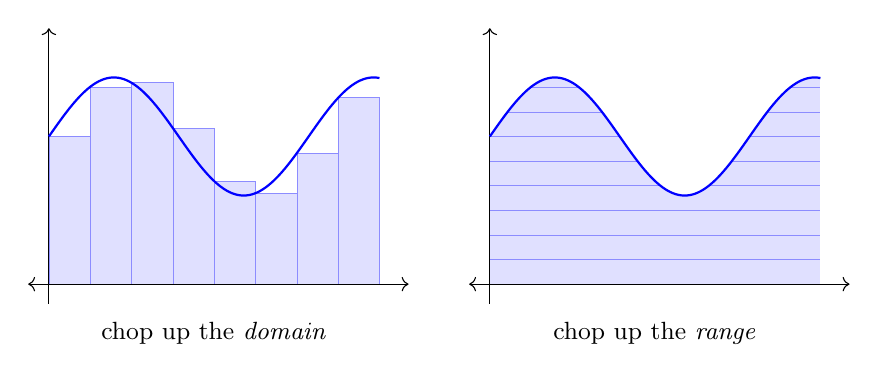
\begin{tikzpicture}[x=1.05cm, y=1.25cm]
	% ---- Riemann: vertical strips ----
	\begin{scope}
	\foreach \a/\h in {0/1.5, 0.5/2.005, 1.0/2.046, 1.5/1.585, 2.0/1.046, 2.5/0.925, 3.0/1.332, 3.5/1.894}{
		\draw[fill=blue!12, draw=blue!45, very thin] (\a,0) rectangle ({\a+0.5},\h);
	}
	\draw[<->] (-0.25,0) -- (4.35,0);
	\draw[->] (0,-0.2) -- (0,2.6);
	\draw[thick, smooth, samples=120, color=blue, domain=0:4] plot (\x, {1.5+0.6*sin(2*\x r)});
	\node[font=\small] at (2,-0.5) {chop up the \emph{domain}};
	\end{scope}
	% ---- Lebesgue: horizontal slabs ----
	\begin{scope}[xshift=5.6cm]
	\begin{scope}
		\clip plot[smooth, samples=120, domain=0:4] (\x, {1.5+0.6*sin(2*\x r)}) -- (4,0) -- (0,0) -- cycle;
		\fill[blue!12] (0,0) rectangle (4,2.3);
		\foreach \y in {0.25,0.5,...,2.25}{
			\draw[blue!45, very thin] (0,\y) -- (4,\y);
		}
	\end{scope}
	\draw[<->] (-0.25,0) -- (4.35,0);
	\draw[->] (0,-0.2) -- (0,2.6);
	\draw[thick, smooth, samples=120, color=blue, domain=0:4] plot (\x, {1.5+0.6*sin(2*\x r)});
	\node[font=\small] at (2,-0.5) {chop up the \emph{range}};
	\end{scope}
\end{tikzpicture}
\end{center}

So the plan for the first third of the course is forced upon us. We must decide which sets get a size (\S2), we must decide which functions are compatible with that assignment (\S3), and only then can we build the integral (\S4). It is worth saying at the outset that the first of these steps is the hard one, and that it cannot be done perfectly: we will prove in \S2 that there is no way to assign a length to \emph{every} subset of $\R$ in a translation-invariant, countably additive way. Some sets must be left out. Deciding exactly which ones is the content of the Carath\'eodory extension theorem, and it will occupy us for a while.

\section{Measures}

\subsection{Set systems}

Throughout, $E$ is a non-empty set, and we write $\mathcal{P}(E)$ for its power set. We want to specify a family of subsets of $E$ -- the sets to which we are prepared to assign a size -- and we want that family to be closed under the operations we expect to perform. The right notion is the following.

\begin{definition}[$\sigma$-algebra]
	A collection $\cE \subseteq \mathcal{P}(E)$ is a \vocab{$\sigma$-algebra} on $E$ if
	\begin{enumerate}[label=(\roman*)]
		\item $\varnothing \in \cE$;
		\item $A \in \cE$ implies $A^c = E \setminus A \in \cE$;
		\item if $(A_n)_{n \in \N}$ is a sequence in $\cE$ then $\bigcup_{n} A_n \in \cE$.
	\end{enumerate}
	The pair $(E, \cE)$ is then called a \vocab{measurable space}, and the elements of $\cE$ are called \vocab{measurable sets}.
\end{definition}

Note that $E = \varnothing^c \in \cE$, and that by De Morgan
$$
\bigcap_n A_n = \Big( \bigcup_n A_n^c \Big)^c \in \cE,
$$
so $\sigma$-algebras are closed under countable intersections as well as countable unions; and $B \setminus A = B \cap A^c \in \cE$, so they are closed under set difference too. The prefix $\sigma$ is there to record the fact that we allow \emph{countable} unions, and this is exactly the right amount of infinity: finite unions are too weak to say anything about limits, and uncountable unions would be far too strong (every subset of $\R$ is an uncountable union of singletons).

\begin{example}[Two extreme examples]
	The collection $\{\varnothing, E\}$ is a $\sigma$-algebra, the smallest one. The power set $\mathcal{P}(E)$ is a $\sigma$-algebra, the largest one. Neither is very useful on its own: the first is too coarse to distinguish anything, and we will see that the second is too fine to admit a sensible notion of length on $\R$.
\end{example}

In practice one rarely writes down a $\sigma$-algebra explicitly. Instead one specifies a handful of sets one certainly wants to be measurable, and takes the smallest $\sigma$-algebra containing them.

\begin{definition}[Generated $\sigma$-algebra]
	Let $\cA \subseteq \mathcal{P}(E)$. The \vocab{$\sigma$-algebra generated by $\cA$} is
	$$
	\sigma(\cA) = \bigcap \{ \cE : \cE \text{ is a $\sigma$-algebra on } E, \; \cA \subseteq \cE \}.
	$$
\end{definition}

This is well defined because $\mathcal{P}(E)$ is a $\sigma$-algebra containing $\cA$, so the intersection is over a non-empty family; and an arbitrary intersection of $\sigma$-algebras is easily checked to be a $\sigma$-algebra. By construction $\sigma(\cA)$ is the smallest $\sigma$-algebra containing $\cA$.

\begin{definition}[Borel $\sigma$-algebra]
	Let $(E, \tau)$ be a topological space. The \vocab{Borel $\sigma$-algebra} on $E$ is $\cB(E) = \sigma(\tau)$, the $\sigma$-algebra generated by the open sets. Its elements are the \vocab{Borel sets}. We abbreviate $\cB = \cB(\R)$.
\end{definition}

The Borel $\sigma$-algebra on $\R$ contains every open set, every closed set, every countable intersection of open sets, every countable union of those, and so on -- one really does have to work to write down a subset of $\R$ that is not Borel. (We will manage it, with the help of the axiom of choice, in \S2.7.)

\begin{example}[Generators of $\cB$]
	Each of the following families generates $\cB$:
	$$
	\{ (a,b) : a<b \}, \quad \{ (a, b] : a < b \}, \quad \{ (-\infty, y] : y \in \R \}, \quad \{ (q, r) : q < r,\; q,r \in \Q \}.
	$$
	For the last of these: every open subset of $\R$ is a countable union of rational intervals, so $\sigma(\{(q,r)\}) \supseteq \tau$ and hence contains $\cB$; and each $(q,r)$ is open, so the reverse containment holds too. For the third, $(-\infty, y] = \bigcap_n (-\infty, y + 1/n)$ is Borel, and conversely $(a,b) = \bigcup_n \big( (-\infty, b - 1/n] \setminus (-\infty, a] \big)$.
\end{example}

Working directly with $\sigma$-algebras is unpleasant, because the countable operations make it hard to verify anything by hand. It is much more comfortable to work with systems closed only under finitary operations, and then to bootstrap. The following two definitions give the finitary systems that we will use as generators.

\begin{definition}[Ring and algebra]
	A collection $\cA \subseteq \mathcal{P}(E)$ is a \vocab{ring} on $E$ if $\varnothing \in \cA$ and, for all $A, B \in \cA$, both $B \setminus A \in \cA$ and $A \cup B \in \cA$.

	It is an \vocab{algebra} on $E$ if $\varnothing \in \cA$ and, for all $A, B \in \cA$, both $A^c \in \cA$ and $A \cup B \in \cA$.
\end{definition}

\begin{remark}
	Every algebra is a ring, since $B \setminus A = (B^c \cup A)^c$. The converse fails: a ring need not contain $E$ itself. For instance the finite unions of bounded intervals of the form $(a,b]$ form a ring on $\R$ but not an algebra. Rings are closed under intersection, because $A \cap B = (A \cup B) \setminus \big( (A\setminus B) \cup (B \setminus A)\big)$, and hence under symmetric difference as well.
\end{remark}

The following triviality gets used so often that it deserves a name.

\begin{proposition}[Disjointification]\label{prop:disjointify}
	Let $\cA$ be a ring and let $A_1, A_2, \dots \in \cA$. Then there are pairwise disjoint $B_1, B_2, \dots \in \cA$ with $B_n \subseteq A_n$ and
	$$
	\bigcup_{n \leq N} A_n = \bigcup_{n \leq N} B_n \quad \text{for every } N,
	$$
	and consequently $\bigcup_n A_n = \bigcup_n B_n$.
\end{proposition}
\begin{proof}
	Set $B_1 = A_1$ and $B_{n+1} = A_{n+1} \setminus (A_1 \cup \cdots \cup A_n)$, which lies in $\cA$ since rings are closed under finite unions and differences. These are disjoint, and an easy induction gives the displayed identity.
\end{proof}

\subsection{Measures}

We can now say what a size function is.

\begin{definition}[Measure]
	Let $(E, \cE)$ be a measurable space. A \vocab{measure} on $(E, \cE)$ is a function $\mu : \cE \to [0, \infty]$ such that $\mu(\varnothing) = 0$ and, for every sequence $(A_n)_{n\in\N}$ of \emph{pairwise disjoint} sets in $\cE$,
	$$
	\mu\Big( \bigcup_{n \in \N} A_n \Big) = \sum_{n \in \N} \mu(A_n).
	$$
	This last property is \vocab{countable additivity}. The triple $(E, \cE, \mu)$ is a \vocab{measure space}.
\end{definition}

We allow the value $+\infty$; the sum on the right is a sum of non-negative terms, so it converges in $[0,\infty]$ regardless of order, and there is no ambiguity. A measure is \vocab{finite} if $\mu(E) < \infty$, and \vocab{$\sigma$-finite} if $E = \bigcup_n E_n$ for some $E_n \in \cE$ with $\mu(E_n) < \infty$. It is a \vocab{probability measure} if $\mu(E) = 1$.

\begin{example}[Counting measure and Dirac measure]
	On $(E, \mathcal{P}(E))$, define $\mu(A) = |A|$ if $A$ is finite and $\infty$ otherwise. This is the \vocab{counting measure}. Fix $x \in E$ and define $\delta_x(A) = 1$ if $x \in A$ and $0$ otherwise; this is the \vocab{Dirac measure} at $x$, a probability measure.
\end{example}

\begin{remark}
	If $E$ is countable and $\cE = \mathcal{P}(E)$, then any measure is determined by its values on singletons: $\mu(A) = \sum_{x \in A} \mu(\{x\})$ by countable additivity. This is exactly the notion of a probability mass function from IA Probability. It is the uncountable case that requires all the machinery.
\end{remark}

Countable additivity is a strong assumption, and it immediately gives us the properties we would expect of a notion of size.

\begin{proposition}[Basic properties of measures]\label{prop:measure-basic}
	Let $(E, \cE, \mu)$ be a measure space and let $A, B, A_n \in \cE$.
	\begin{enumerate}[label=(\roman*)]
		\item (Monotonicity) If $A \subseteq B$ then $\mu(A) \leq \mu(B)$.
		\item (Countable subadditivity) $\mu\big( \bigcup_n A_n \big) \leq \sum_n \mu(A_n)$.
		\item (Continuity from below) If $A_n \uparrow A$, meaning $A_1 \subseteq A_2 \subseteq \cdots$ and $A = \bigcup_n A_n$, then $\mu(A_n) \to \mu(A)$.
		\item (Continuity from above) If $A_n \downarrow A$ and $\mu(A_1) < \infty$, then $\mu(A_n) \to \mu(A)$.
	\end{enumerate}
\end{proposition}
\begin{proof}
	(i) Write $B = A \sqcup (B \setminus A)$; then $\mu(B) = \mu(A) + \mu(B\setminus A) \geq \mu(A)$.

	(ii) Disjointify as in Proposition \ref{prop:disjointify} to get disjoint $B_n \subseteq A_n$ with the same union. Then
	$$
	\mu\Big( \bigcup_n A_n \Big) = \mu\Big( \bigsqcup_n B_n \Big) = \sum_n \mu(B_n) \leq \sum_n \mu(A_n)
	$$
	using monotonicity in the last step.

	(iii) Set $B_1 = A_1$ and $B_{n+1} = A_{n+1} \setminus A_n$; these are disjoint with $\bigcup_{n \leq N} B_n = A_N$ and $\bigcup_n B_n = A$. So
	$$
	\mu(A) = \sum_{n=1}^\infty \mu(B_n) = \lim_{N \to \infty} \sum_{n=1}^N \mu(B_n) = \lim_{N\to\infty} \mu(A_N).
	$$

	(iv) Apply (iii) to $A_1 \setminus A_n \uparrow A_1 \setminus A$. This gives $\mu(A_1) - \mu(A_n) \to \mu(A_1) - \mu(A)$, and since $\mu(A_1) < \infty$ we may cancel.
\end{proof}

The finiteness hypothesis in (iv) is genuinely needed: with $\mu$ the counting measure on $\N$ and $A_n = \{n, n+1, \dots\}$ we have $A_n \downarrow \varnothing$ but $\mu(A_n) = \infty$ for every $n$.

We will eventually want to build measures by prescribing them on some convenient family of sets and extending. For that we need to talk about functions defined on families that are not $\sigma$-algebras.

\begin{definition}[Set function]
	Let $\cA \subseteq \mathcal{P}(E)$ with $\varnothing \in \cA$. A \vocab{set function} on $\cA$ is a map $\mu : \cA \to [0,\infty]$ with $\mu(\varnothing) = 0$. We call $\mu$
	\begin{enumerate}[label=(\roman*)]
		\item \vocab{increasing} if $\mu(A) \leq \mu(B)$ whenever $A \subseteq B$ with $A, B \in \cA$;
		\item \vocab{additive} if $\mu(A \cup B) = \mu(A) + \mu(B)$ whenever $A, B \in \cA$ are disjoint and $A \cup B \in \cA$;
		\item \vocab{countably additive} if $\mu(\bigcup_n A_n) = \sum_n \mu(A_n)$ whenever the $A_n \in \cA$ are pairwise disjoint and $\bigcup_n A_n \in \cA$;
		\item \vocab{countably subadditive} if $\mu(\bigcup_n A_n) \leq \sum_n \mu(A_n)$ whenever $A_n \in \cA$ and $\bigcup_n A_n \in \cA$.
	\end{enumerate}
\end{definition}

On a ring, countable additivity implies all of the others, by exactly the arguments of Proposition \ref{prop:measure-basic}. A measure is precisely a countably additive set function on a $\sigma$-algebra.

\subsection{\texorpdfstring{$\pi$}{pi}-systems, \texorpdfstring{$d$}{d}-systems and Dynkin's lemma}

Here is the difficulty we are about to face repeatedly. We will want to prove that two measures agree on a $\sigma$-algebra $\cE$, knowing only that they agree on some generating family $\cA$. The natural strategy is to consider $\cD = \{A : \mu_1(A) = \mu_2(A)\}$ and show it is a $\sigma$-algebra containing $\cA$. Unfortunately $\cD$ is \emph{not} obviously a $\sigma$-algebra: additivity gives us nothing about $\mu_i(A \cup B)$ when $A$ and $B$ overlap. What $\cD$ \emph{is} closed under is proper differences and increasing limits. This motivates the following.

\begin{definition}[$\pi$-system]
	A collection $\cA \subseteq \mathcal{P}(E)$ is a \vocab{$\pi$-system} if $\varnothing \in \cA$ and $A, B \in \cA$ implies $A \cap B \in \cA$.
\end{definition}

\begin{definition}[$d$-system]
	A collection $\cD \subseteq \mathcal{P}(E)$ is a \vocab{$d$-system} (or Dynkin system) if
	\begin{enumerate}[label=(\roman*)]
		\item $E \in \cD$;
		\item if $B_1, B_2 \in \cD$ with $B_1 \subseteq B_2$, then $B_2 \setminus B_1 \in \cD$;
		\item if $A_n \in \cD$ with $A_n \uparrow A$, then $A \in \cD$.
	\end{enumerate}
\end{definition}

The point of the pair of definitions is that they are complementary: neither alone is a $\sigma$-algebra, but together they are.

\begin{center}
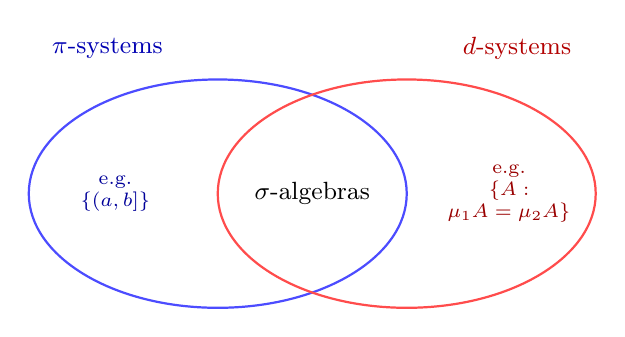
\begin{tikzpicture}[scale=1]
	\draw[thick, blue!70] (-1.2,0) ellipse (2.4 and 1.45);
	\draw[thick, red!70] (1.2,0) ellipse (2.4 and 1.45);
	\node[blue!70!black, font=\small] at (-2.6,1.85) {$\pi$-systems};
	\node[red!70!black, font=\small] at (2.6,1.85) {$d$-systems};
	\node[font=\small] at (0,0) {$\sigma$-algebras};
	\node[font=\scriptsize, blue!60!black, align=center] at (-2.5,0) {e.g.\\ $\{(a,b]\}$};
	\node[font=\scriptsize, red!60!black, align=center] at (2.5,0) {e.g.\\ $\{A :$\\ $\mu_1 A = \mu_2 A\}$};
\end{tikzpicture}
\end{center}

\begin{proposition}\label{prop:pi-d-sigma}
	A collection which is both a $\pi$-system and a $d$-system is a $\sigma$-algebra.
\end{proposition}
\begin{proof}
	Let $\cD$ be both. Then $E \in \cD$, and taking $B_1 = A$, $B_2 = E$ in (ii) gives $A^c \in \cD$; in particular $\varnothing = E^c \in \cD$. For countable unions, let $A_n \in \cD$. Since $\cD$ is a $\pi$-system and is closed under complements, it is closed under finite unions:
	$$
	A \cup B = (A^c \cap B^c)^c \in \cD.
	$$
	So $\tilde A_N = A_1 \cup \cdots \cup A_N \in \cD$, and $\tilde A_N \uparrow \bigcup_n A_n$, whence $\bigcup_n A_n \in \cD$ by (iii).
\end{proof}

The engine of the whole subject is now the following lemma, which says that to check a property holds on $\sigma(\cA)$ it is enough to check that the class of sets with that property is a $d$-system, provided $\cA$ is a $\pi$-system.

\begin{lemma}[Dynkin's lemma]\label{lem:dynkin}
	Let $\cA$ be a $\pi$-system. Then any $d$-system containing $\cA$ contains $\sigma(\cA)$.
\end{lemma}
\begin{proof}
	Let $\cD$ be the intersection of all $d$-systems containing $\cA$; one checks immediately that an intersection of $d$-systems is a $d$-system, so $\cD$ is the smallest $d$-system containing $\cA$, and it suffices to show $\sigma(\cA) \subseteq \cD$. By Proposition \ref{prop:pi-d-sigma} it is enough to show that $\cD$ is a $\pi$-system, for then $\cD$ is a $\sigma$-algebra containing $\cA$ and hence contains $\sigma(\cA)$.

	The trick is to do this in two steps. First set
	$$
	\cD' = \{ B \in \cD : B \cap A \in \cD \text{ for all } A \in \cA \}.
	$$
	We claim $\cD'$ is a $d$-system. Certainly $E \in \cD'$, since $E \cap A = A \in \cA \subseteq \cD$. If $B_1 \subseteq B_2$ both lie in $\cD'$ then for $A \in \cA$,
	$$
	(B_2 \setminus B_1) \cap A = (B_2 \cap A) \setminus (B_1 \cap A),
	$$
	a proper difference of elements of $\cD$, hence in $\cD$; so $B_2 \setminus B_1 \in \cD'$. If $B_n \uparrow B$ with $B_n \in \cD'$ then $B_n \cap A \uparrow B \cap A$, so $B \cap A \in \cD$ and $B \in \cD'$. Finally $\cA \subseteq \cD'$, precisely because $\cA$ is a $\pi$-system. By minimality of $\cD$ we get $\cD \subseteq \cD'$, and the reverse inclusion is by definition, so $\cD' = \cD$.

	Now set
	$$
	\cD'' = \{ B \in \cD : B \cap A \in \cD \text{ for all } A \in \cD \}.
	$$
	Exactly the same three verifications show $\cD''$ is a $d$-system. And $\cA \subseteq \cD''$: for $A \in \cA$ and $B \in \cD = \cD'$ we have $B \cap A \in \cD$, which is what membership of $A$ in $\cD''$ requires. So again $\cD'' = \cD$ by minimality, and this says exactly that $\cD$ is closed under intersections.
\end{proof}

The first payoff is immediate.

\begin{theorem}[Uniqueness of extension]\label{pm-thm:uniqueness}
	Let $(E, \cE)$ be a measurable space and let $\mu_1, \mu_2$ be measures on it. Suppose $\cA \subseteq \cE$ is a $\pi$-system with $\sigma(\cA) = \cE$, that $\mu_1 = \mu_2$ on $\cA$, and that $E \in \cA$ with $\mu_1(E) = \mu_2(E) < \infty$. Then $\mu_1 = \mu_2$ on $\cE$.
\end{theorem}
\begin{proof}
	Let $\cD = \{ A \in \cE : \mu_1(A) = \mu_2(A)\}$. By hypothesis $\cA \subseteq \cD$, so by Dynkin's lemma it suffices to show $\cD$ is a $d$-system.

	We have $E \in \cD$ by assumption. If $B_1 \subseteq B_2$ lie in $\cD$ then, using additivity and the finiteness of $\mu_i(B_1) \leq \mu_i(E) < \infty$ to justify the subtraction,
	$$
	\mu_1(B_2 \setminus B_1) = \mu_1(B_2) - \mu_1(B_1) = \mu_2(B_2) - \mu_2(B_1) = \mu_2(B_2 \setminus B_1),
	$$
	so $B_2 \setminus B_1 \in \cD$. Finally if $A_n \uparrow A$ with $A_n \in \cD$, then by continuity from below
	$$
	\mu_1(A) = \lim_n \mu_1(A_n) = \lim_n \mu_2(A_n) = \mu_2(A),
	$$
	so $A \in \cD$.
\end{proof}

\begin{remark}
	The finiteness assumption cannot be dropped outright -- take $\mu_1$ counting measure and $\mu_2 = 2\mu_1$ on $(\R, \cB)$, which agree (both being $\infty$) on the $\pi$-system of non-empty open intervals. But it can be relaxed to $\sigma$-finiteness: if $E = \bigcup_n E_n$ with $E_n \in \cA$ increasing and $\mu_1(E_n) = \mu_2(E_n) < \infty$, apply the theorem to $A \mapsto \mu_i(A \cap E_n)$ for each $n$ and let $n \to \infty$. We will use it in this form for Lebesgue measure.
\end{remark}

\subsection{The Carath\'eodory extension theorem}

We now come to the existence half of the story. The situation we have in mind is this: on the ring $\cA$ of finite unions of half-open intervals $(a,b] \subseteq \R$, there is an obvious candidate for length, namely the sum of the lengths of the intervals. We would like to promote it to a measure on $\sigma(\cA) = \cB$. Carath\'eodory's theorem says that this is always possible, provided the candidate is countably additive on the ring to begin with.

\begin{theorem}[Carath\'eodory extension theorem]\label{thm:caratheodory}
	Let $\cA$ be a ring on $E$ and let $\mu$ be a countably additive set function on $\cA$. Then $\mu$ extends to a measure on $\sigma(\cA)$.
\end{theorem}

The proof is long but the idea is simple and worth stating first. We define an \emph{outer measure} $\mu^\star$ on \emph{all} subsets of $E$ by covering them as efficiently as possible with sets from $\cA$. This $\mu^\star$ is defined everywhere but is only subadditive, not additive. We then cut down to the class $\cM$ of sets which `split every set additively', and show that on this class $\mu^\star$ is a genuine measure and that $\cM \supseteq \cA$ -- hence $\cM \supseteq \sigma(\cA)$, and we are done.

\begin{proof}
	For $B \subseteq E$ define the \vocab{outer measure}
	$$
	\mu^\star(B) = \inf \Big\{ \sum_{n \in \N} \mu(A_n) \; : \; A_n \in \cA, \; B \subseteq \bigcup_{n \in \N} A_n \Big\},
	$$
	with the convention $\mu^\star(B) = \infty$ if no such countable cover exists. Note $\mu^\star(\varnothing) = 0$ and $\mu^\star$ is increasing. Define the \vocab{$\mu^\star$-measurable sets}
	$$
	\cM = \big\{ A \subseteq E \; : \; \mu^\star(B) = \mu^\star(B \cap A) + \mu^\star(B \cap A^c) \text{ for all } B \subseteq E \big\}.
	$$
	We proceed in five steps.

	\textbf{Step 1: $\mu^\star$ is countably subadditive on $\mathcal{P}(E)$.} Let $B \subseteq \bigcup_n B_n$; we must show
	\begin{equation}\label{eq:cara-dagger}
		\mu^\star(B) \leq \sum_n \mu^\star(B_n). \tag{$\dagger$}
	\end{equation}
	We may assume every $\mu^\star(B_n) < \infty$. Fix $\varepsilon > 0$. For each $n$, choose $A_{n,m} \in \cA$ with $B_n \subseteq \bigcup_m A_{n,m}$ and
	$$
	\sum_m \mu(A_{n,m}) \leq \mu^\star(B_n) + \varepsilon 2^{-n}.
	$$
	Then $\{A_{n,m}\}_{n,m}$ is a countable cover of $B$ by elements of $\cA$, so
	$$
	\mu^\star(B) \leq \sum_{n,m} \mu(A_{n,m}) \leq \sum_n \mu^\star(B_n) + \varepsilon.
	$$
	As $\varepsilon>0$ was arbitrary, \eqref{eq:cara-dagger} holds.

	\textbf{Step 2: $\mu^\star$ extends $\mu$.} Let $A \in \cA$. Covering $A$ by $A, \varnothing, \varnothing, \dots$ gives $\mu^\star(A) \leq \mu(A)$. Conversely, suppose $A \subseteq \bigcup_n A_n$ with $A_n \in \cA$. Then $A = \bigcup_n (A \cap A_n)$ is a countable union of elements of $\cA$; since $\mu$ is countably additive on the ring $\cA$ it is countably subadditive there, so
	$$
	\mu(A) \leq \sum_n \mu(A \cap A_n) \leq \sum_n \mu(A_n).
	$$
	Taking the infimum over covers, $\mu(A) \leq \mu^\star(A)$.

	\textbf{Step 3: $\cA \subseteq \cM$.} Let $A \in \cA$ and $B \subseteq E$. The inequality $\mu^\star(B) \leq \mu^\star(B \cap A) + \mu^\star(B\cap A^c)$ is immediate from \eqref{eq:cara-dagger}. For the reverse, we may assume $\mu^\star(B) < \infty$. Fix $\varepsilon > 0$ and choose $A_n \in \cA$ with $B \subseteq \bigcup_n A_n$ and $\sum_n \mu(A_n) \leq \mu^\star(B) + \varepsilon$. Now $B \cap A \subseteq \bigcup_n (A_n \cap A)$ and $B \cap A^c \subseteq \bigcup_n (A_n \setminus A)$, and both $A_n \cap A$ and $A_n \setminus A$ lie in the ring $\cA$. Hence
	\begin{align*}
		\mu^\star(B\cap A) + \mu^\star(B \cap A^c) &\leq \sum_n \mu(A_n \cap A) + \sum_n \mu(A_n \setminus A) \\
		&= \sum_n \big[ \mu(A_n \cap A) + \mu(A_n \setminus A) \big] = \sum_n \mu(A_n) \leq \mu^\star(B) + \varepsilon,
	\end{align*}
	using additivity of $\mu$ on $\cA$. Let $\varepsilon \to 0$.

	\textbf{Step 4: $\cM$ is an algebra.} That $\varnothing \in \cM$ is clear, and the definition of $\cM$ is symmetric in $A$ and $A^c$, so $\cM$ is closed under complements. For intersections, let $A_1, A_2 \in \cM$ and $B \subseteq E$. Applying the defining identity for $A_1$ and then for $A_2$ (with test set $B \cap A_1$),
	$$
	\mu^\star(B) = \mu^\star(B \cap A_1 \cap A_2) + \mu^\star(B \cap A_1 \cap A_2^c) + \mu^\star(B\cap A_1^c).
	$$
	Now observe $A_1 \cap A_2^c = (A_1 \cap A_2)^c \cap A_1$ and $A_1^c = (A_1\cap A_2)^c \cap A_1^c$, so the last two terms are
	$$
	\mu^\star\big(B \cap (A_1\cap A_2)^c \cap A_1\big) + \mu^\star\big(B \cap (A_1 \cap A_2)^c \cap A_1^c\big) = \mu^\star\big(B \cap (A_1\cap A_2)^c\big),
	$$
	using that $A_1 \in \cM$ with test set $B \cap (A_1 \cap A_2)^c$. Hence
	$$
	\mu^\star(B) = \mu^\star(B \cap (A_1 \cap A_2)) + \mu^\star(B \cap (A_1\cap A_2)^c),
	$$
	so $A_1 \cap A_2 \in \cM$.

	\textbf{Step 5: $\cM$ is a $\sigma$-algebra and $\mu^\star$ is a measure on it.} Let $A = \bigcup_n A_n$ with $A_n \in \cM$; by Step 4 and disjointification we may assume the $A_n$ are disjoint. Let $B \subseteq E$. Applying the defining identity repeatedly and using disjointness (so that $B \cap A_1^c \cap A_2 = B \cap A_2$, and so on),
	\begin{align*}
		\mu^\star(B) &= \mu^\star(B\cap A_1) + \mu^\star(B \cap A_1^c) \\
		&= \mu^\star(B\cap A_1) + \mu^\star(B\cap A_2) + \mu^\star(B \cap A_1^c \cap A_2^c) \\
		&= \cdots = \sum_{n \leq N} \mu^\star(B \cap A_n) + \mu^\star\Big( B \cap \bigcap_{n \leq N} A_n^c \Big).
	\end{align*}
	Since $\bigcap_{n \leq N} A_n^c \supseteq A^c$ and $\mu^\star$ is increasing, the last term is at least $\mu^\star(B \cap A^c)$. Letting $N \to \infty$,
	$$
	\mu^\star(B) \geq \sum_{n=1}^\infty \mu^\star(B \cap A_n) + \mu^\star(B \cap A^c) \geq \mu^\star(B \cap A) + \mu^\star(B \cap A^c),
	$$
	the last step by \eqref{eq:cara-dagger}. The reverse inequality is \eqref{eq:cara-dagger} again, so $A \in \cM$ and $\cM$ is a $\sigma$-algebra. Moreover, taking $B = A$ in the display above gives
	$$
	\mu^\star(A) \geq \sum_{n=1}^\infty \mu^\star(A_n),
	$$
	and the reverse holds by subadditivity, so $\mu^\star$ is countably additive on $\cM$.

	Combining Steps 3 and 5, $\cM$ is a $\sigma$-algebra containing $\cA$, so $\sigma(\cA) \subseteq \cM$; and by Step 2 the measure $\mu^\star|_{\sigma(\cA)}$ extends $\mu$.
\end{proof}

\begin{remark}
	The class $\cM$ is generally strictly larger than $\sigma(\cA)$. In the case of Lebesgue measure on $\R$ it is the class of \vocab{Lebesgue measurable} sets, and one can show
	$$
	\cM = \{ A \cup N : A \in \cB, \; N \subseteq B \text{ for some } B \in \cB \text{ with } \mu(B) = 0 \} \supsetneq \cB.
	$$
	In words, $\cM$ is obtained from $\cB$ by throwing in all subsets of null sets; it is the \vocab{completion} of $\cB$. There is no harm in working with $\cB$ throughout, and it is more convenient, so we shall.
\end{remark}
\subsection{Lebesgue measure}

We can now build the measure that started it all. The construction on $\R$ is the substantial one; higher dimensions will follow painlessly from the theory of product measures in \S5.

\begin{theorem}[Lebesgue measure on $\R$]\label{pm-thm:lebesgue}
	There is a unique Borel measure $\mu$ on $\R$ with
	$$
	\mu\big( (a,b] \big) = b - a \qquad \text{for all } a < b.
	$$
	We call $\mu$ \vocab{Lebesgue measure}.
\end{theorem}
\begin{proof}
	Let $\cA$ consist of $\varnothing$ together with all sets of the form
	$$
	A = (a_1, b_1] \cup \cdots \cup (a_n, b_n]
	$$
	with the intervals disjoint and $-\infty < a_i < b_i < \infty$. This $\cA$ is a ring: the difference and union of two such sets is again such a set. It is also a $\pi$-system, and $\sigma(\cA) = \cB$, since every open interval $(a,b) = \bigcup_n (a, b - 1/n]$ lies in $\sigma(\cA)$ and the open intervals generate $\cB$.

	Define $\mu(A) = \sum_{i=1}^n (b_i - a_i)$ for $A$ as above. This is well defined: if $A = \bigsqcup_j C_j = \bigsqcup_k D_k$ are two such representations then, writing $C_j = \bigsqcup_k (C_j \cap D_k)$ and $D_k = \bigsqcup_j (C_j \cap D_k)$ and using additivity of length on intervals,
	$$
	\sum_j \mathrm{len}(C_j) = \sum_j \sum_k \mathrm{len}(C_j \cap D_k) = \sum_k \sum_j \mathrm{len}(C_j \cap D_k) = \sum_k \mathrm{len}(D_k).
	$$
	Additivity of $\mu$ on $\cA$ is then clear.

	To apply Carath\'eodory we must upgrade additivity to \emph{countable} additivity on $\cA$. For a finitely additive set function on a ring, countable additivity is equivalent to the statement that $\mu(A_n) \to 0$ whenever $A_n \in \cA$ with $A_n \downarrow \varnothing$. (Indeed, if $\bigsqcup_n B_n = B \in \cA$ then $A_N = B \setminus \bigsqcup_{n \leq N} B_n \downarrow \varnothing$ and $\mu(B) = \sum_{n \leq N}\mu(B_n) + \mu(A_N)$.) So suppose for contradiction that $B_n \in \cA$ with $B_n \downarrow \varnothing$ but $\mu(B_n) \geq 2\varepsilon$ for all $n$, for some $\varepsilon > 0$.

	The idea is to shrink each $B_n$ slightly to a set whose closure is still inside $B_n$, and then use compactness. Write $B_n = \bigsqcup_{i=1}^{N_n} (a_{ni}, b_{ni}]$ and put
	$$
	C_n = \bigsqcup_{i=1}^{N_n} \Big( a_{ni} + \tfrac{2^{-n}\varepsilon}{N_n},\; b_{ni} \Big] \in \cA,
	$$
	so that $\overline{C_n} \subseteq B_n$ and $\mu(B_n \setminus C_n) \leq 2^{-n}\varepsilon$. Since the $B_n$ decrease, $B_N = \bigcap_{n \leq N} B_n$, and so
	$$
	B_N \setminus (C_1 \cap \cdots \cap C_N) = \bigcup_{n \leq N} (B_N \setminus C_n) \subseteq \bigcup_{n\leq N} (B_n \setminus C_n),
	$$
	giving $\mu\big( B_N \setminus (C_1 \cap \cdots \cap C_N)\big) \leq \sum_{n \leq N} 2^{-n}\varepsilon \leq \varepsilon$. As $\mu(B_N) \geq 2\varepsilon$, additivity forces
	$$
	\mu(C_1 \cap \cdots \cap C_N) \geq \varepsilon > 0,
	$$
	so in particular $C_1 \cap \cdots \cap C_N \neq \varnothing$ for every $N$. Setting $K_N = \overline{C_1} \cap \cdots \cap \overline{C_N}$, we obtain a decreasing sequence of non-empty compact subsets of $\R$, so by the finite intersection property there is $x \in \bigcap_N K_N$. But $K_N \subseteq \overline{C_N} \subseteq B_N$, so $x \in \bigcap_N B_N = \varnothing$, a contradiction. Hence $\mu$ is countably additive on $\cA$, and Carath\'eodory gives a measure on $\sigma(\cA) = \cB$ extending it.

	For uniqueness, suppose $\mu, \lambda$ are two Borel measures assigning length $b-a$ to $(a,b]$. For each $n \in \Z$ the measures $A \mapsto \mu(A \cap (n, n+1])$ and $A \mapsto \lambda(A \cap (n,n+1])$ are finite measures of total mass $1$ agreeing on the $\pi$-system $\cA$, so they agree on $\cB$ by Theorem \ref{pm-thm:uniqueness}. Summing over $n \in \Z$ and using countable additivity, $\mu = \lambda$.
\end{proof}

\begin{definition}[Null set]
	A set $N \in \cE$ with $\mu(N) = 0$ is called \vocab{$\mu$-null}. A property is said to hold \vocab{$\mu$-almost everywhere} (abbreviated a.e.) if the set where it fails is contained in a null set.
\end{definition}

\begin{example}[Countable sets are Lebesgue null]
	For $x \in \R$ we have $\{x\} = \bigcap_n (x - 1/n, x]$, a decreasing intersection of sets of finite measure, so by continuity from above $\mu(\{x\}) = \lim_n 1/n = 0$. Hence any countable set is null, being a countable union of null sets. In particular $\mu(\Q) = 0$, and
	$$
	\mu\big((a,b)\big) = \mu\big([a,b]\big) = \mu\big((a,b]\big) = b - a.
	$$
	Not every null set is countable: the Cantor middle-thirds set is uncountable and has measure $\lim_n (2/3)^n = 0$.
\end{example}

\begin{proposition}[Translation invariance]
	For $x \in \R$ and $B \in \cB$ we have $B + x \in \cB$ and $\mu(B+x) = \mu(B)$.
\end{proposition}
\begin{proof}
	The map $y \mapsto y - x$ is a homeomorphism of $\R$, so $B \mapsto B + x$ preserves $\cB$. Define $\mu_x(B) = \mu(B+x)$. This is a Borel measure and $\mu_x((a,b]) = \mu((a+x, b+x]) = b-a$. By the uniqueness in Theorem \ref{pm-thm:lebesgue}, $\mu_x = \mu$.
\end{proof}

Since Lebesgue measure is the unique translation-invariant Borel measure normalised by $\mu((0,1]) = 1$, translation invariance is really the defining property, and it is what we will exploit in the next subsection to show that not every set can be measured.

\subsection{Measures from distribution functions}

Before that, it is worth recording that essentially the same construction gives every reasonable measure on $\R$ at once. Recall that a Borel measure $\mu$ on a Hausdorff space $E$ is called a \vocab{Radon measure} if $\mu(K)$ is finite for every compact set $K \subseteq E$. Note that compact subsets of a Hausdorff space are closed, and hence Borel.

\begin{lemma}[Generalised inverse]\label{lem:gen-inverse}
	Let $g : \R \to \R$ be non-decreasing and right-continuous, and put
	$$
	g(-\infty) = \lim_{y \to -\infty} g(y), \qquad g(+\infty) = \lim_{y\to\infty}g(y).
	$$
	On the open interval $I = \big(g(-\infty), g(+\infty)\big)$ define
	$$
	f(x) = \inf\{ y \in \R : x \leq g(y)\}.
	$$
	Then $f$ is non-decreasing and left-continuous, and for $x \in I$, $y \in \R$,
	$$
	f(x) \leq y \iff x \leq g(y).
	$$
\end{lemma}
\begin{proof}
	Let $J_x = \{y \in \R : x \leq g(y)\}$. Since $x > g(-\infty)$ the set $J_x$ is bounded below, and since $x < g(+\infty)$ it is non-empty; so $f(x) \in \R$. If $y \in J_x$ and $y' \geq y$ then $y' \in J_x$ as $g$ is non-decreasing, so $J_x$ is an up-set. If $y_n \downarrow y$ with $y_n \in J_x$, then $x \leq g(y_n) \to g(y)$ by right-continuity, so $y \in J_x$. Hence $J_x$ is closed and $J_x = [f(x), \infty)$, which is exactly the stated equivalence.

	If $x \leq x'$ then $J_{x} \supseteq J_{x'}$, so $f(x) \leq f(x')$. If $x_n \uparrow x$ then $J_x = \bigcap_n J_{x_n}$, so $f(x_n) \uparrow f(x)$, giving left-continuity.
\end{proof}

\begin{theorem}[Lebesgue--Stieltjes measures]\label{thm:stieltjes}
	Let $g : \R \to \R$ be non-decreasing and right-continuous. Then there is a unique Radon measure $\mu_g$ on $\R$ with
	$$
	\mu_g\big((a,b]\big) = g(b) - g(a) \qquad (a<b),
	$$
	and every Radon measure on $\R$ arises this way.
\end{theorem}
\begin{proof}
	The construction of Theorem \ref{pm-thm:lebesgue} goes through verbatim with $b - a$ replaced by $g(b)-g(a)$, right-continuity of $g$ being exactly what is needed to make the shrinking argument work. Alternatively -- and this is the slicker route -- let $f$ be the generalised inverse of Lemma \ref{lem:gen-inverse}. For $z \in \R$,
	$$
	f^{-1}\big((-\infty, z]\big) = \{x \in I : f(x)\leq z\} = \{x \in I : x \leq g(z)\} = I \cap (-\infty, g(z)],
	$$
	which is Borel; since the sets $(-\infty,z]$ generate $\cB$, the map $f$ is measurable (see \S3.1). Let $\mu$ be Lebesgue measure restricted to $I$ and set $\mu_g = \mu \circ f^{-1}$. This is a measure, and
	$$
	\mu_g\big((a,b]\big) = \mu\big(\{x : a < f(x) \leq b\}\big) = \mu\big(\{x : g(a) < x \leq g(b)\}\big) = g(b)-g(a).
	$$
	Uniqueness follows as before. Any compact set lies in some $[a,b]$, whose measure $g(b)-g(a)$ is finite, so $\mu_g$ is Radon.

	Conversely, given a Radon measure $\nu$ on $\R$, define $g(y) = \nu((0,y])$ for $y \geq 0$ and $g(y) = -\nu((y,0])$ for $y<0$. Then $g$ is non-decreasing, right-continuous by continuity from above, and $\nu((a,b]) = g(b)-g(a)$ by additivity; uniqueness gives $\nu = \mu_g$.
\end{proof}

We call $g$ the \vocab{Stieltjes distribution function} of $\mu_g$. Taking $g(y)=y$ recovers Lebesgue measure; taking $g = \ind_{[x,\infty)}$ recovers the Dirac measure $\delta_x$. When $\mu_g$ is a probability measure this $g$ is exactly the distribution function of a random variable, as we will see in \S3.

\subsection{A non-measurable set}

We now show that our caution was justified: one cannot extend Lebesgue measure to all of $\mathcal{P}(\R)$. The construction is due to Vitali and uses the axiom of choice in an essential way.

Work on $E = (0,1]$ with addition modulo $1$; concretely, identify $E$ with the circle $\R/\Z$. Lebesgue measure restricted to $E$ is invariant under this addition: for $B \subseteq E$ Borel and $x \in E$, the set $B \oplus x$ is a translate of $B \cap (0, 1-x]$ union a translate of $B \cap (1-x, 1]$, and both pieces keep their measure.

Let $Q = E \cap \Q$, a countable subgroup of $(E, \oplus)$. Define $x \sim y$ iff $x - y \in \Q$; this is an equivalence relation, whose classes are the cosets $x \oplus Q$. By the axiom of choice, pick one representative from each class and let $S$ be the resulting set. Then
$$
E = \bigsqcup_{q \in Q} (S \oplus q),
$$
a \emph{disjoint} union: every $x \in E$ lies in the class of exactly one representative, and if $S \oplus q$ met $S \oplus q'$ with $q \neq q'$ then $S$ would contain two representatives of the same class.

\begin{center}
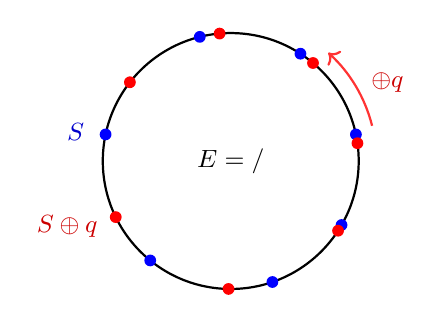
\begin{tikzpicture}[scale=1.25]
	\draw[thick] (0,0) circle (1.3);
	\foreach \a in {12, 57, 104, 168, 231, 289, 330}{
		\fill[blue] (\a:1.3) circle (1.7pt);
	}
	\foreach \a in {12, 57, 104, 168, 231, 289, 330}{
		\fill[red] ({\a+38}:1.3) circle (1.7pt);
	}
	\draw[->, red!80, thick] (14:1.48) arc (14:48:1.48);
	\node[red!80!black, font=\small, anchor=west] at (31:1.55) {$\oplus q$};
	\node[blue!80!black, font=\small, anchor=east] at (168:1.42) {$S$};
	\node[red!80!black, font=\small, anchor=east] at (208:1.42) {$S \oplus q$};
	\node[font=\small] at (0,0) {$E = \R/\Z$};
\end{tikzpicture}
\end{center}

\begin{theorem}[Vitali]
	The set $S$ is not Lebesgue measurable. Consequently there is no translation-invariant measure defined on all of $\mathcal{P}\big((0,1]\big)$ giving the whole space measure $1$.
\end{theorem}
\begin{proof}
	Suppose $S$ were measurable with $\mu(S) = c$. Each translate $S \oplus q$ is then measurable with the same measure $c$, and by countable additivity
	$$
	1 = \mu(E) = \sum_{q \in Q} \mu(S \oplus q) = \sum_{q\in Q} c.
	$$
	If $c = 0$ the sum is $0$; if $c > 0$ the sum is $\infty$ (as $Q$ is infinite). Either way we cannot get $1$, a contradiction.
\end{proof}

\begin{remark}
	One can go further. Assuming the continuum hypothesis, a theorem of Banach and Kuratowski says that there is \emph{no} measure at all on $\mathcal{P}((0,1])$ with $\mu((0,1]) = 1$ and $\mu(\{x\}) = 0$ for every $x$ -- translation invariance is not even needed. So the restriction to a $\sigma$-algebra is not an artefact of our construction; it is unavoidable.
\end{remark}

\subsection{Probability spaces and independence}

Everything we have done so far specialises to probability by the simple device of normalising the total mass.

\begin{definition}[Probability space]
	A measure space $(E, \cE, \mu)$ with $\mu(E) = 1$ is a \vocab{probability space}. We change notation to $(\Omega, \cF, \PP)$ and call $\Omega$ the \vocab{sample space}, elements of $\cF$ \vocab{events}, and $\PP$ the \vocab{probability measure}.
\end{definition}

Kolmogorov's axioms of probability, as laid down in 1933, say precisely that $\PP(\Omega)=1$, that $0 \leq \PP(A) \leq 1$, and that $\PP$ is countably additive. So a probability space is nothing more than a measure space of total mass one -- there is no new content, only new vocabulary. The reader who recalls the continuity properties of $\PP$ from IA Probability will recognise Proposition \ref{prop:measure-basic} as the general form of those results.

\begin{definition}[Independence]
	Events $(A_i)_{i \in I}$ in $\cF$ are \vocab{independent} if for every finite $J \subseteq I$,
	$$
	\PP\Big( \bigcap_{j\in J} A_j \Big) = \prod_{j \in J} \PP(A_j).
	$$
	Sub-$\sigma$-algebras $(\cA_i)_{i \in I}$ of $\cF$ are \vocab{independent} if, whenever $J \subseteq I$ is finite and $A_j \in \cA_j$ for $j \in J$, the events $(A_j)_{j \in J}$ are independent.
\end{definition}

Checking independence of $\sigma$-algebras directly is hopeless, but Dynkin's lemma reduces it to a check on generators.

\begin{proposition}\label{prop:indep-pi}
	Let $\cA_1, \cA_2$ be $\pi$-systems contained in $\cF$ with $\Omega \in \cA_1 \cap \cA_2$. Suppose
	$$
	\PP(A_1 \cap A_2) = \PP(A_1)\PP(A_2) \qquad \text{for all } A_1 \in \cA_1, \; A_2 \in \cA_2.
	$$
	Then $\sigma(\cA_1)$ and $\sigma(\cA_2)$ are independent.
\end{proposition}
\begin{proof}
	Fix $A_2 \in \cA_2$ and consider the two finite measures $B \mapsto \PP(B \cap A_2)$ and $B \mapsto \PP(B)\PP(A_2)$ on $\sigma(\cA_1)$. They agree on the $\pi$-system $\cA_1$ and have the same total mass $\PP(A_2)$, so by Theorem \ref{pm-thm:uniqueness} they agree on $\sigma(\cA_1)$. Now fix $B \in \sigma(\cA_1)$ and repeat the argument in the second coordinate: the measures $C \mapsto \PP(B \cap C)$ and $C \mapsto \PP(B)\PP(C)$ agree on the $\pi$-system $\cA_2$, hence on $\sigma(\cA_2)$.
\end{proof}

\subsection{The Borel--Cantelli lemmas}

Given a sequence of events $(A_n)$, two sets naturally record its asymptotic behaviour.

\begin{definition}[Limsup and liminf of events]
	For $A_n \in \cF$ we define
	$$
	\limsup_n A_n = \bigcap_{n} \bigcup_{m \geq n} A_m = \{A_n \text{ i.o.}\},\qquad
	\liminf_n A_n = \bigcup_n \bigcap_{m\geq n} A_m = \{A_n \text{ ev.}\}.
	$$
\end{definition}

Unwinding the quantifiers: $\omega \in \limsup_n A_n$ iff for every $n$ there is some $m \geq n$ with $\omega \in A_m$, that is, iff $\omega$ lies in infinitely many of the $A_n$. Similarly $\omega \in \liminf_n A_n$ iff $\omega$ lies in all but finitely many. Both sets are in $\cF$.

\begin{center}
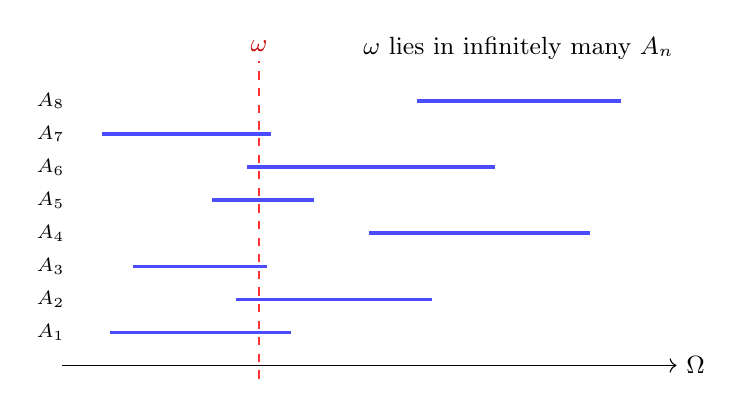
\begin{tikzpicture}[x=1cm, y=0.42cm]
	\draw[->] (-0.3,0) -- (7.5,0) node[right, font=\small] {$\Omega$};
	\foreach \n/\a/\b in {1/0.3/2.6, 2/1.9/4.4, 3/0.6/2.3, 4/3.6/6.4, 5/1.6/2.9, 6/2.05/5.2, 7/0.2/2.35, 8/4.2/6.8}{
		\draw[very thick, blue!70] (\a, \n) -- (\b, \n);
		\node[left, font=\scriptsize] at (-0.15, \n) {$A_{\n}$};
	}
	\draw[dashed, red!80, thick] (2.2,-0.4) -- (2.2, 9.2);
	\node[red!80!black, font=\small, above] at (2.2, 9.2) {$\omega$};
	\node[font=\small, align=left, anchor=west] at (3.4, 9.6) {$\omega$ lies in infinitely many $A_n$};
\end{tikzpicture}
\end{center}

The picture to keep in mind is the one above: draw $\Omega$ horizontally, draw each $A_n$ at height $n$, and a point $\omega$ belongs to $\limsup_n A_n$ exactly when the vertical line through $\omega$ meets infinitely many of the segments. The two Borel--Cantelli lemmas give complementary criteria for whether this happens.

\begin{lemma}[First Borel--Cantelli lemma]\label{lem:bc1}
	Let $(A_n)$ be events with $\sum_n \PP(A_n) < \infty$. Then $\PP(A_n \text{ i.o.}) = 0$.
\end{lemma}
\begin{proof}
	For every $n$,
	$$
	\PP\Big( \bigcap_{k} \bigcup_{m\geq k} A_m \Big) \leq \PP\Big( \bigcup_{m \geq n} A_m \Big) \leq \sum_{m\geq n} \PP(A_m),
	$$
	and the right-hand side is the tail of a convergent series, so tends to $0$ as $n \to \infty$.
\end{proof}

Note that this proof never used $\PP(\Omega)=1$; the lemma holds for an arbitrary measure $\mu$ in place of $\PP$, and we will use it in that generality.

\begin{lemma}[Second Borel--Cantelli lemma]\label{lem:bc2}
	Let $(A_n)$ be \emph{independent} events with $\sum_n \PP(A_n) = \infty$. Then $\PP(A_n \text{ i.o.}) = 1$.
\end{lemma}
\begin{proof}
	Fix $n$. By independence and the elementary inequality $1 - a \leq e^{-a}$,
	$$
	\PP\Big( \bigcap_{m=n}^N A_m^c \Big) = \prod_{m=n}^N \big(1 - \PP(A_m)\big) \leq \exp\Big( - \sum_{m=n}^N \PP(A_m) \Big) \longrightarrow 0
	$$
	as $N \to \infty$, since the series diverges. The sets $\bigcap_{m=n}^N A_m^c$ decrease to $\bigcap_{m \geq n} A_m^c$ as $N \to \infty$, so $\PP\big( \bigcap_{m\geq n} A_m^c \big) = 0$ for every $n$. Hence
	$$
	\PP\big( (A_n \text{ i.o.})^c \big) = \PP\Big( \bigcup_n \bigcap_{m \geq n} A_m^c \Big) \leq \sum_n \PP\Big( \bigcap_{m\geq n} A_m^c\Big) = 0. \qedhere
	$$
\end{proof}

The two lemmas together are a remarkably sharp tool: for independent events, $\PP(A_n \text{ i.o.})$ is $0$ or $1$ according to whether $\sum_n \PP(A_n)$ converges or diverges, with no intermediate case. Here is a typical application, which we can state now and will be able to re-derive later.

\begin{example}[Records of exponential variables]\label{ex:exp-records}
	Let $(X_n)$ be independent with $\PP(X_1 > x) = e^{-x}$ for $x \geq 0$, and let $\alpha > 0$. Put $A_n = \{X_n \geq \alpha \log n\}$, so $\PP(A_n) = n^{-\alpha}$. Then $\sum_n \PP(A_n) < \infty$ iff $\alpha > 1$. By the two lemmas, for every $\varepsilon>0$,
	$$
	\PP\Big( \frac{X_n}{\log n} \geq 1 \text{ i.o.} \Big) = 1, \qquad \PP\Big( \frac{X_n}{\log n} \geq 1 + \varepsilon \text{ i.o.}\Big) = 0.
	$$
	Combining, $\limsup_n X_n / \log n = 1$ almost surely. So the record values of an i.i.d.\ exponential sequence grow exactly logarithmically.
\end{example}

\section{Measurable Functions and Random Variables}

\subsection{Measurable functions}

Having decided which sets we can measure, we must decide which functions respect that structure. As always in mathematics, the right notion of morphism is the one that pulls structure back.

\begin{definition}[Measurable function]
	Let $(E, \cE)$ and $(G, \cG)$ be measurable spaces. A function $f : E \to G$ is \vocab{$\cE$-$\cG$ measurable} (or just \vocab{measurable}) if
	$$
	f^{-1}(A) \in \cE \qquad \text{for every } A \in \cG.
	$$
\end{definition}

When $G = \R$ with $\cG = \cB$, we simply say $f$ is measurable; when in addition $E$ is a topological space and $\cE = \cB(E)$, we say $f$ is \vocab{Borel measurable}. Note the analogy with continuity, which is the statement that preimages of open sets are open.

The saving grace is that measurability can be checked on generators, because preimages commute with all the set operations: $f^{-1}(A^c) = f^{-1}(A)^c$ and $f^{-1}(\bigcup_n A_n) = \bigcup_n f^{-1}(A_n)$.

\begin{lemma}[Measurability on generators]\label{lem:meas-gen}
	Let $\cG = \sigma(\cA)$. If $f^{-1}(A) \in \cE$ for every $A \in \cA$, then $f$ is measurable.
\end{lemma}
\begin{proof}
	The collection $\{A \subseteq G : f^{-1}(A) \in \cE\}$ is a $\sigma$-algebra on $G$, by the displayed identities. It contains $\cA$ by hypothesis, hence contains $\sigma(\cA) = \cG$.
\end{proof}

\begin{example}[Useful special cases]
	\begin{enumerate}[label=(\roman*)]
		\item A function $f : (E,\cE) \to \R$ is measurable if and only if $\{x : f(x) \leq y\} \in \cE$ for every $y \in \R$, since the sets $(-\infty,y]$ generate $\cB$.
		\item If $E$ is a topological space with $\cE = \cB(E)$ and $f : E \to \R$ is continuous, then $f$ is measurable: preimages of open sets are open, hence Borel, and open sets generate $\cB$.
		\item The indicator $\ind_A$ is measurable if and only if $A \in \cE$, since $\ind_A^{-1}(\{1\}) = A$.
	\end{enumerate}
\end{example}

\begin{proposition}[Stability of measurability]\label{prop:meas-stable}
	Let $f, g, f_n : (E,\cE) \to \R$ be measurable and $\lambda \in \R$. Then the following are measurable:
	$$
	f + g, \quad fg, \quad \lambda f, \quad \max(f,g), \quad \min(f,g), \quad \inf_n f_n, \quad \sup_n f_n, \quad \liminf_n f_n, \quad \limsup_n f_n,\!\!
	$$
	the last four taking values in $[-\infty,\infty]$. Moreover the composition of measurable functions is measurable.
\end{proposition}
\begin{proof}
	Composition is immediate: $(g \circ f)^{-1}(A) = f^{-1}(g^{-1}(A))$.

	For the supremum, $\{\sup_n f_n \leq y\} = \bigcap_n \{f_n \leq y\} \in \cE$; for the infimum, $\{\inf_n f_n < y\} = \bigcup_n \{f_n < y\} \in \cE$. Then $\liminf_n f_n = \sup_n \inf_{m \geq n} f_m$ and $\limsup_n f_n = \inf_n \sup_{m \geq n} f_m$ are measurable, and $\max, \min$ of two functions are special cases.

	For sums, note $\{f + g > y\} = \bigcup_{q \in \Q} \big( \{f > q\} \cap \{g > y - q\}\big) \in \cE$. For products, $fg = \frac{1}{4}\big[(f+g)^2 - (f-g)^2\big]$, so it suffices to know $h^2$ is measurable when $h$ is, and this follows from $\{h^2 \leq y\} = \{-\sqrt y \leq h \leq \sqrt y\}$ for $y \geq 0$.
\end{proof}

That last proposition is worth pausing over. It says that measurability -- unlike continuity, or differentiability, or Riemann integrability -- is preserved under \emph{pointwise limits}. This is exactly the robustness we were missing, and it is the reason the Lebesgue theory has the convergence theorems it does.

We single out the functions which will serve as building blocks.

\begin{definition}[Simple function]
	A function $f : (E,\cE) \to \R$ is \vocab{simple} if it can be written as
	$$
	f = \sum_{k=1}^m a_k \ind_{A_k}, \qquad a_k \geq 0, \; A_k \in \cE, \; m \in \N.
	$$
	Equivalently, $f$ is measurable, non-negative, and takes only finitely many values.
\end{definition}

The following approximation is the single most used construction in the course; we will refer to it as \emph{the standard approximation}.

\begin{proposition}[Approximation by simple functions]\label{prop:std-approx}
	Let $f : (E,\cE) \to [0,\infty]$ be measurable. Define
	$$
	f_n = 2^{-n}\lfloor 2^n f \rfloor \wedge n = \sum_{j=0}^{n2^n - 1} \frac{j}{2^n}\ind_{A_{n,j}} + n \ind_{\{f \geq n\}}, \qquad A_{n,j} = f^{-1}\Big( \Big[ \frac{j}{2^n}, \frac{j+1}{2^n}\Big)\Big).
	$$
	Then each $f_n$ is simple, $0 \leq f_n \leq f_{n+1} \leq f$, and $f_n \to f$ pointwise. If $f$ is bounded the convergence is uniform, with $\|f - f_n\|_\infty \leq 2^{-n}$ once $n > \|f\|_\infty$.
\end{proposition}
\begin{proof}
	Each $A_{n,j}$ lies in $\cE$ by measurability of $f$, so $f_n$ is simple. Monotonicity in $n$ holds because refining the mesh from $2^{-n}$ to $2^{-(n+1)}$ can only increase the value of $\lfloor \cdot \rfloor$-rounding downwards, and because the truncation level $n$ increases. If $f(x) < \infty$ then for $n > f(x)$ we have $0 \leq f(x) - f_n(x) \leq 2^{-n}$, and if $f(x) = \infty$ then $f_n(x) = n \to \infty$.
\end{proof}

\begin{center}
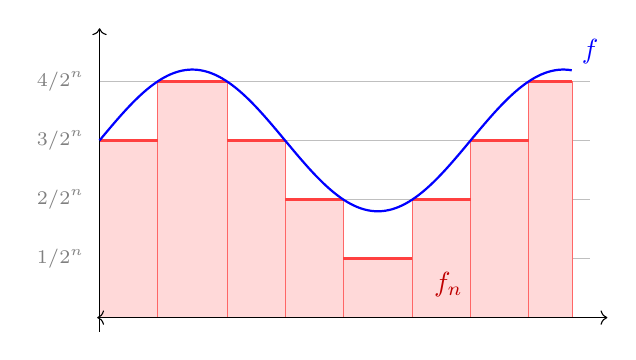
\begin{tikzpicture}[x=1.5cm, y=1.5cm]
	% level lines
	\foreach \y/\lab in {0.5/{1}, 1.0/{2}, 1.5/{3}, 2.0/{4}}{
		\draw[lightgray, thin] (0,\y) -- (4.15,\y);
		\node[left, font=\scriptsize, gray] at (-0.05,\y) {$\lab/2^n$};
	}
	% staircase pieces
	\foreach \a/\b/\h in {0/0.4926/1.5, 0.4926/1.0783/2.0, 1.0783/1.5708/1.5, 1.5708/2.0633/1.0, 2.0633/2.649/0.5, 2.649/3.1416/1.0, 3.1416/3.634/1.5, 3.634/4/2.0}{
		\draw[fill=red!15, draw=red!60, very thin] (\a,0) rectangle (\b,\h);
	}
	\foreach \a/\b/\h in {0/0.4926/1.5, 0.4926/1.0783/2.0, 1.0783/1.5708/1.5, 1.5708/2.0633/1.0, 2.0633/2.649/0.5, 2.649/3.1416/1.0, 3.1416/3.634/1.5, 3.634/4/2.0}{
		\draw[very thick, red!75] (\a,\h) -- (\b,\h);
	}
	\draw[<->] (-0.02,0) -- (4.3,0);
	\draw[->] (0,-0.12) -- (0,2.45);
	\draw[thick, smooth, samples=140, color=blue, domain=0:4] plot (\x, {1.5+0.6*sin(2*\x r)});
	\node[blue, right] at (4.0, 2.25) {$f$};
	\node[red!75!black, right] at (2.75, 0.28) {$f_n$};
\end{tikzpicture}
\end{center}

The picture shows the staircase $f_n$ sitting underneath $f$. Everything we prove about the integral will be proved first for simple functions, where it is a finite computation, and then transported to general non-negative $f$ along this staircase using the monotone convergence theorem.

\subsection{The monotone class theorem}

Dynkin's lemma has a functional analogue which will let us prove statements about all bounded measurable functions by checking them only on indicators of a $\pi$-system.

\begin{theorem}[Monotone class theorem]\label{thm:mct-class}
	Let $\cA$ be a $\pi$-system generating $\cE$, with $E \in \cA$. Let $\cV$ be a vector space of bounded functions $E \to \R$ such that
	\begin{enumerate}[label=(\roman*)]
		\item $\ind_E \in \cV$ and $\ind_A \in \cV$ for all $A \in \cA$;
		\item if $f_n \in \cV$ are non-negative with $f_n \uparrow f$ pointwise and $f$ is bounded, then $f \in \cV$.
	\end{enumerate}
	Then $\cV$ contains every bounded measurable function $f: (E,\cE) \to \R$.
\end{theorem}
\begin{proof}
	Let $\cD = \{A \in \cE : \ind_A \in \cV\}$. Then $E \in \cD$ and $\cA \subseteq \cD$. If $A \subseteq B$ with $A,B \in \cD$ then $\ind_{B\setminus A} = \ind_B - \ind_A \in \cV$ since $\cV$ is a vector space. If $A_n \uparrow A$ with $A_n \in \cD$ then $\ind_{A_n} \uparrow \ind_A$, which is bounded, so $\ind_A \in \cV$ by (ii). Hence $\cD$ is a $d$-system containing the $\pi$-system $\cA$, and Dynkin's lemma gives $\cD = \cE$.

	Now let $f$ be bounded, measurable and non-negative, and let $f_n$ be its standard approximation from Proposition \ref{prop:std-approx}. Each $f_n$ is a finite non-negative linear combination of indicators of sets in $\cE = \cD$, hence lies in $\cV$; and $f_n \uparrow f$ with $f$ bounded, so $f \in \cV$ by (ii). For general bounded measurable $f$, write $f = f^+ - f^-$ with $f^\pm = \max(\pm f, 0)$ bounded, measurable and non-negative; both lie in $\cV$, hence so does $f$.
\end{proof}

\subsection{Image measures and random variables}

A measurable function transports a measure forwards.

\begin{definition}[Image measure]
	Let $f : (E,\cE) \to (G,\cG)$ be measurable and $\mu$ a measure on $(E,\cE)$. The \vocab{image measure} (or pushforward) is
	$$
	(\mu \circ f^{-1})(A) = \mu\big(f^{-1}(A)\big), \qquad A \in \cG.
	$$
\end{definition}

That this is a measure is immediate: preimages preserve disjointness and commute with countable unions.

\begin{definition}[Random variable]
	Let $(\Omega, \cF, \PP)$ be a probability space and $(E,\cE)$ a measurable space. An \vocab{$E$-valued random variable} is a measurable map $X : (\Omega, \cF) \to (E,\cE)$. When $E = \R$ (or $\R^d$) with the Borel $\sigma$-algebra we simply say \vocab{random variable} (or random vector).

	The \vocab{law} or \vocab{distribution} of $X$ is the image measure $\mu_X = \PP \circ X^{-1}$, a probability measure on $(E,\cE)$.
\end{definition}

We also write $\sigma(X) = \{X^{-1}(A) : A \in \cE\}$, the $\sigma$-algebra \emph{generated by} $X$; it is the smallest $\sigma$-algebra on $\Omega$ making $X$ measurable, and morally it encodes exactly the information one learns by observing $X$.

\begin{definition}[Distribution function]
	For a real-valued random variable $X$, the \vocab{distribution function} is
	$$
	F_X(z) = \mu_X\big((-\infty,z]\big) = \PP(X \leq z).
	$$
\end{definition}

Since the intervals $(-\infty,z]$ form a $\pi$-system generating $\cB$, and $\mu_X$ is a probability measure, Theorem \ref{pm-thm:uniqueness} tells us that $F_X$ determines $\mu_X$ completely. From the properties of measures we read off that $F_X$ is non-decreasing, right-continuous (by continuity from above), with $F_X(z) \to 0$ as $z \to -\infty$ and $F_X(z) \to 1$ as $z \to \infty$. Conversely, given any such $F$, Lemma \ref{lem:gen-inverse} produces a random variable with that distribution function: take $(\Omega,\cF,\PP) = ((0,1), \cB((0,1)), \mu)$ and $X(\omega) = \inf\{x : \omega \leq F(x)\}$, so that $\PP(X \leq z) = \mu(\{\omega : \omega \leq F(z)\}) = F(z)$. This is the \emph{inverse transform} construction familiar from simulation.

\begin{definition}[Independent random variables]
	A family $(X_i)_{i \in I}$ of random variables on $(\Omega,\cF,\PP)$ is \vocab{independent} if the $\sigma$-algebras $\sigma(X_i)$ are independent.
\end{definition}

For real-valued $X_i$ the sets $\{X_i \leq x\}$ form a $\pi$-system generating $\sigma(X_i)$, so by Proposition \ref{prop:indep-pi} (extended to finitely many systems in the obvious way) independence is equivalent to
$$
\PP(X_1 \leq x_1, \dots, X_n \leq x_n) = \prod_{i=1}^n \PP(X_i \leq x_i)
$$
for all finite subfamilies and all $x_i \in \R$. This is the criterion one actually uses.

\subsection{Constructing independent random variables}

It is not obvious that an infinite sequence of independent random variables with prescribed laws exists at all. Happily, one probability space suffices for everything: the unit interval with Lebesgue measure.

Take $(\Omega, \cF, \PP) = \big((0,1), \cB((0,1)), \mu\big)$. Every $\omega \in (0,1)$ has a binary expansion $\omega = \sum_{n\geq 1} \omega_n 2^{-n}$, unique if we forbid expansions ending in all $1$s. Define the \vocab{Rademacher functions}
$$
R_n(\omega) = \omega_n \in \{0,1\}.
$$
Each $R_n$ is a finite sum of indicators of dyadic intervals, hence measurable, and $\PP(R_n = 1) = \PP(R_n = 0) = 1/2$. For any $x_1,\dots,x_n \in \{0,1\}$, the event $\{R_1 = x_1,\dots,R_n = x_n\}$ is a single dyadic interval of length $2^{-n}$, so
$$
\PP(R_1 = x_1, \dots, R_n = x_n) = 2^{-n} = \prod_{i=1}^n \PP(R_i = x_i),
$$
and the $R_n$ are independent Bernoulli$(1/2)$ variables.

Now take a bijection $m : \N^2 \to \N$ and set $Y_{n,k} = R_{m(n,k)}$; these are again independent. Define
$$
Y_n = \sum_{k=1}^\infty 2^{-k} Y_{n,k},
$$
which converges everywhere. The $Y_n$ are independent, being functions of disjoint sub-families of the $R_m$. Moreover each $Y_n$ is uniform on $(0,1)$: for the dyadic intervals $\big(i2^{-m}, (i+1)2^{-m}\big]$, which form a $\pi$-system generating $\cB((0,1))$,
$$
\PP\Big( Y_n \in \big(i2^{-m}, (i+1)2^{-m}\big] \Big) = 2^{-m},
$$
since this event prescribes the first $m$ binary digits of $Y_n$. By uniqueness of extension, $Y_n \sim U(0,1)$.

Finally, given any sequence $(F_n)$ of distribution functions, let $g_n$ be the generalised inverse of $F_n$ from Lemma \ref{lem:gen-inverse}. Then $X_n = g_n(Y_n)$ is a sequence of independent random variables with $\PP(X_n \leq x) = \PP(Y_n \leq F_n(x)) = F_n(x)$. So:

\begin{theorem}\label{thm:construct-iid}
	Given any sequence $(F_n)$ of distribution functions there is a probability space carrying a sequence of independent random variables $(X_n)$ with $X_n$ having distribution function $F_n$. In particular i.i.d.\ sequences of any prescribed law exist.
\end{theorem}

\subsection{Convergence of measurable functions}

Two notions of convergence make sense at this level of generality.

\begin{definition}[Almost everywhere and in measure]
	Let $f_n, f$ be measurable functions on $(E,\cE,\mu)$. We say $f_n \to f$ \vocab{almost everywhere} if $\mu(\{x : f_n(x) \not\to f(x)\}) = 0$, and $f_n \to f$ \vocab{in measure} if for every $\varepsilon > 0$,
	$$
	\mu\big( \{ x : |f_n(x) - f(x)| > \varepsilon\}\big) \to 0 \quad \text{as } n \to \infty.
	$$
	On a probability space these are called convergence \vocab{almost surely} and \vocab{in probability}, and we write $X_n \to X$ a.s.\ and $X_n \xrightarrow{\PP} X$.
\end{definition}

\begin{theorem}[Relations between the two]\label{thm:ae-vs-measure}
	Let $f_n$ be measurable on $(E,\cE,\mu)$.
	\begin{enumerate}[label=(\roman*)]
		\item If $\mu(E) < \infty$ and $f_n \to 0$ a.e., then $f_n \to 0$ in measure.
		\item If $f_n \to 0$ in measure, then $f_{n_k} \to 0$ a.e.\ along some subsequence $(n_k)$.
	\end{enumerate}
\end{theorem}
\begin{proof}
	(i) Fix $\varepsilon > 0$. The sets $B_n = \bigcap_{m \geq n} \{|f_m| \leq \varepsilon\}$ increase, with
	$$
	\bigcup_n B_n = \{|f_n| \leq \varepsilon \text{ eventually}\} \supseteq \{f_n \to 0\},
	$$
	a set of full measure. By continuity from below, $\mu(B_n) \to \mu(E)$. Since $\mu(\{|f_n| \leq \varepsilon\}) \geq \mu(B_n)$ and $\mu(E) < \infty$, we may subtract to get $\mu(\{|f_n| > \varepsilon\}) \leq \mu(E) - \mu(B_n) \to 0$.

	(ii) For each $k$, convergence in measure with $\varepsilon = 1/k$ lets us choose $n_k$ (increasing) with
	$$
	\mu\big( |f_{n_k}| > 1/k \big) \leq 2^{-k}.
	$$
	Then $\sum_k \mu(|f_{n_k}| > 1/k) < \infty$, so by the first Borel--Cantelli lemma (valid for any measure) the set where $|f_{n_k}| > 1/k$ infinitely often is null. Off that set, $|f_{n_k}| \leq 1/k$ eventually, so $f_{n_k}\to 0$.
\end{proof}

Both hypotheses are needed, as the following show.

\begin{example}[Two counterexamples]
	\begin{enumerate}[label=(\roman*)]
		\item On $(\R, \cB, \mu)$ let $f_n = \ind_{(n,\infty)}$. Then $f_n \to 0$ pointwise, but $\mu(|f_n| > 1/2) = \infty$ for every $n$. So (i) genuinely needs $\mu(E)<\infty$.
		\item Let $(A_n)$ be independent events with $\PP(A_n)= 1/n$. Then $\ind_{A_n}\to 0$ in probability, since $\PP(\ind_{A_n} > \varepsilon) = 1/n \to 0$. But $\sum_n \PP(A_n) = \infty$, so by the second Borel--Cantelli lemma $\PP(A_n \text{ i.o.}) = 1$ and $\ind_{A_n} \not\to 0$ almost surely. So (ii) genuinely needs a subsequence.
	\end{enumerate}
\end{example}

\subsection{Tail events and Kolmogorov's zero-one law}

Let $(X_n)_{n \in \N}$ be a sequence of random variables. Define
$$
\cT_n = \sigma(X_{n+1}, X_{n+2}, \dots), \qquad \cT = \bigcap_{n \in \N}\cT_n.
$$
We call $\cT$ the \vocab{tail $\sigma$-algebra}. An event in $\cT$ is one whose occurrence is unaffected by changing any finite number of the $X_n$ -- for instance $\{X_n \to 0\}$, or $\{\sum_n X_n \text{ converges}\}$, or $\{\limsup_n \frac1n\sum_{i\leq n} X_i > c\}$. Kolmogorov's theorem says that for independent $X_n$ such events are deterministic.

\begin{theorem}[Kolmogorov's zero-one law]\label{thm:kolmogorov01}
	Let $(X_n)$ be independent random variables and let $A \in \cT$. Then $\PP(A) \in \{0,1\}$. Moreover any $\cT$-measurable random variable $Y$ is almost surely constant.
\end{theorem}
\begin{proof}
	Let $\cF_n = \sigma(X_1,\dots,X_n)$, which is generated by the $\pi$-system of events of the form $\{X_1 \leq x_1, \dots, X_n\leq x_n\}$; and note that $\cT_n$ is generated by the $\pi$-system of events of the form $\{X_{n+1}\leq x_{n+1},\dots,X_{n+k}\leq x_{n+k}\}$, for $k \in \N$. By independence of the $X_i$ these two $\pi$-systems satisfy the product rule, so by Proposition \ref{prop:indep-pi} the $\sigma$-algebras $\cF_n$ and $\cT_n$ are independent.

	Let $\cF_\infty = \sigma(X_1, X_2, \dots)$. Then $\bigcup_n \cF_n$ is a $\pi$-system (the $\cF_n$ increase) generating $\cF_\infty$. Any $A \in \bigcup_n \cF_n$ lies in some $\cF_n$, hence is independent of $\cT_n \supseteq \cT$. So $\bigcup_n \cF_n$ and $\cT$ satisfy the product rule, and by Proposition \ref{prop:indep-pi} again, $\cF_\infty$ is independent of $\cT$.

	But $\cT \subseteq \cF_\infty$. So if $A \in \cT$ then $A$ is independent of itself:
	$$
	\PP(A) = \PP(A \cap A) = \PP(A)^2,
	$$
	forcing $\PP(A) \in \{0,1\}$.

	For the last statement, $F_Y(y) = \PP(Y \leq y)$ takes only the values $0$ and $1$, is non-decreasing and right-continuous with limits $0$ and $1$ at $\mp\infty$; so $c = \inf\{y : F_Y(y) = 1\}$ is finite and $Y = c$ almost surely.
\end{proof}

\begin{example}
	If $(X_n)$ are independent then the event that $\sum_n X_n$ converges has probability $0$ or $1$, and $\limsup_n \frac1n \sum_{i=1}^n X_i$ is an almost surely constant element of $[-\infty,\infty]$. The zero-one law does not tell us \emph{which} constant -- that is the work of the laws of large numbers -- but it does tell us that there is no randomness left to speak of.
\end{example}
\section{Integration}

\subsection{Defining the integral}

We now carry out the plan of \S1. Throughout $(E,\cE,\mu)$ is a measure space. We will write the integral of $f$ interchangeably as
$$
\mu(f) = \int_E f \dd\mu = \int_E f(x) \dd\mu(x),
$$
and when $(\Omega,\cF,\PP)$ is a probability space and $X$ a random variable, we write $\EE[X] = \int_\Omega X \dd\PP$ for its \vocab{expectation}. The notation $\mu(f)$ is compact and emphasises that integration is a functional; we will use it freely.

The construction proceeds in three stages: simple functions, non-negative functions, then general functions.

\begin{definition}[Integral of a simple function]
	For a simple function $f = \sum_{k=1}^m a_k \ind_{A_k}$ with $a_k \geq 0$ and $A_k \in \cE$, set
	$$
	\mu(f) = \sum_{k=1}^m a_k \mu(A_k) \; \in [0,\infty].
	$$
\end{definition}

This requires a check: the representation of $f$ is not unique. Suppose $\sum_k a_k \ind_{A_k} = \sum_\ell b_\ell \ind_{B_\ell}$. Refining both into the common refinement generated by the $A_k$ and $B_\ell$ (finitely many sets, so this is a finite disjoint partition) and using finite additivity of $\mu$ on each piece shows both expressions equal the same number. We omit the routine bookkeeping.

\begin{proposition}[The integral on simple functions]\label{prop:int-simple}
	For simple $f,g$ and $\alpha,\beta \geq 0$:
	$$
	\mu(\alpha f + \beta g) = \alpha\mu(f) + \beta\mu(g), \qquad f \leq g \implies \mu(f) \leq \mu(g),
	$$
	$$
	f = 0 \text{ a.e.} \implies \mu(f) = 0.
	$$
\end{proposition}
\begin{proof}
	Linearity is immediate from the definition once one notes that $\alpha f + \beta g$ is again simple with an obvious representation. Monotonicity: if $f \leq g$ then $g - f$ is a non-negative simple function (take a common refinement), so $\mu(g) = \mu(f) + \mu(g-f) \geq \mu(f)$. For the last part, in a representation with the $A_k$ disjoint and $a_k > 0$, we must have $\mu(A_k) = 0$.
\end{proof}

\begin{definition}[Integral of a non-negative function]
	For measurable $f : E \to [0,\infty]$, define
	$$
	\mu(f) = \sup\{ \mu(g) : g \text{ simple}, \; g \leq f \} \; \in [0,\infty].
	$$
\end{definition}

By monotonicity on simple functions this is consistent with the previous definition when $f$ is itself simple. It also makes monotonicity for non-negative $f \leq h$ obvious, since the supremum on the left is over a smaller family.

\begin{definition}[Integrable functions]
	For measurable $f : E \to \R$ write $f^+ = \max(f, 0)$ and $f^- = \max(-f, 0)$, so $f = f^+ - f^-$ and $|f| = f^+ + f^-$. We say $f$ is \vocab{$\mu$-integrable} if $\mu(|f|) < \infty$, and then set
	$$
	\mu(f) = \mu(f^+) - \mu(f^-),
	$$
	a well-defined real number. We write $L^1(\mu)$ for the set of integrable functions.
\end{definition}

Note the asymmetry with the Riemann theory: a function is Lebesgue integrable if and only if its absolute value is. There is no analogue of a conditionally convergent improper integral here; $\int_0^\infty \frac{\sin x}{x}\dd x$ exists as an improper Riemann integral but $\frac{\sin x}{x}$ is not Lebesgue integrable on $(0,\infty)$.

\subsection{The monotone convergence theorem}

Everything now hinges on the following theorem, which is the reason the whole edifice works.

\begin{theorem}[Monotone convergence theorem]\label{pm-thm:mct}
	Let $f_n, f$ be measurable and non-negative with $f_n \uparrow f$ pointwise. Then $\mu(f_n) \uparrow \mu(f)$.
\end{theorem}
\begin{proof}
	Since $f_n \leq f_{n+1} \leq f$, the sequence $\mu(f_n)$ is non-decreasing and bounded above by $\mu(f)$; let $M = \lim_n \mu(f_n) = \sup_n \mu(f_n) \leq \mu(f)$. It remains to prove $\mu(f) \leq M$, i.e.\ that $\mu(g) \leq M$ for every simple $g \leq f$.

	Fix such a $g = \sum_{k=1}^m a_k \ind_{A_k}$ with the $A_k \in \cE$ disjoint and $a_k > 0$, and fix $\varepsilon \in (0,1)$. Put
	$$
	A_k(n) = \{ x \in A_k : f_n(x) \geq (1-\varepsilon)a_k \} \in \cE.
	$$
	Since $f_n \uparrow f \geq g = a_k$ on $A_k$, every $x \in A_k$ eventually satisfies $f_n(x) \geq (1-\varepsilon)a_k$; so $A_k(n) \uparrow A_k$ and, by continuity from below, $\mu(A_k(n)) \uparrow \mu(A_k)$.

	Because the $A_k$ are disjoint,
	$$
	f_n \geq \sum_{k=1}^m f_n \ind_{A_k(n)} \geq (1-\varepsilon)\sum_{k=1}^m a_k \ind_{A_k(n)},
	$$
	and the right-hand side is simple, so
	$$
	\mu(f_n) \geq (1-\varepsilon)\sum_{k=1}^m a_k \mu\big(A_k(n)\big).
	$$
	Letting $n \to \infty$, the right-hand side tends to $(1-\varepsilon)\sum_k a_k \mu(A_k) = (1-\varepsilon)\mu(g)$. Hence $M \geq (1-\varepsilon)\mu(g)$, and letting $\varepsilon \downarrow 0$ gives $M \geq \mu(g)$ as required.
\end{proof}

\begin{remark}
	Three comments. First, this is a theorem about interchanging limits:
	$$
	\mu\big(\lim_n f_n\big) = \lim_n \mu(f_n),
	$$
	something the Riemann integral cannot deliver without uniform convergence. Second, it suffices that $f_n \uparrow f$ almost everywhere -- alter the functions on a null set, which changes no integral. Third, non-negativity is only used to get started; if $f_0$ is integrable and $f_n \uparrow f$ then applying the theorem to $f_n - f_0$ gives the same conclusion.
\end{remark}

Applying the theorem to the standard approximation of Proposition \ref{prop:std-approx} we get, for measurable $f \geq 0$,
$$
\mu(f) = \lim_n \mu\big( 2^{-n}\lfloor 2^n f\rfloor \wedge n \big),
$$
which is a completely explicit recipe: the integral is the limit of the horizontal-slab sums from \S1. It also delivers linearity for free.

\begin{theorem}[Properties of the integral, non-negative case]\label{thm:int-nonneg}
	Let $f, g : E \to [0,\infty]$ be measurable and $\alpha, \beta \geq 0$. Then
	\begin{enumerate}[label=(\roman*)]
		\item $\mu(\alpha f + \beta g) = \alpha \mu(f) + \beta\mu(g)$;
		\item if $f \leq g$ then $\mu(f) \leq \mu(g)$;
		\item $\mu(f) = 0$ if and only if $f = 0$ almost everywhere;
		\item if $g_n \geq 0$ are measurable then $\mu\big(\sum_n g_n\big) = \sum_n \mu(g_n)$.
	\end{enumerate}
\end{theorem}
\begin{proof}
	(i) Let $\tilde f_n \uparrow f$ and $\tilde g_n \uparrow g$ be the standard approximations. Then $\alpha \tilde f_n + \beta\tilde g_n \uparrow \alpha f + \beta g$, and by linearity on simple functions together with the monotone convergence theorem applied three times,
	$$
	\mu(\alpha f + \beta g) = \lim_n \big[\alpha\mu(\tilde f_n) + \beta \mu(\tilde g_n)\big] = \alpha\mu(f)+\beta\mu(g).
	$$

	(ii) Already noted.

	(iii) If $f = 0$ a.e.\ then every simple $g \leq f$ vanishes a.e., so $\mu(g)=0$ and hence $\mu(f)=0$. Conversely suppose $\mu(f)=0$ and let $A_n = \{f > 1/n\}$. Then $\frac1n \ind_{A_n} \leq f$, so $\mu(A_n) \leq n\mu(f) = 0$; and $\{f>0\} = \bigcup_n A_n$ is null.

	(iv) Apply the monotone convergence theorem to the partial sums, using (i) for finite sums.
\end{proof}

\begin{theorem}[Properties of the integral, general case]\label{thm:int-gen}
	Let $f, g \in L^1(\mu)$ and $\alpha,\beta \in \R$. Then $\alpha f + \beta g \in L^1(\mu)$ with $\mu(\alpha f + \beta g) = \alpha \mu(f)+\beta\mu(g)$; if $f \leq g$ then $\mu(f) \leq \mu(g)$; and $|\mu(f)| \leq \mu(|f|)$.
\end{theorem}
\begin{proof}
	For $\alpha \geq 0$, $(\alpha f)^\pm = \alpha f^\pm$ so $\mu(\alpha f) = \alpha\mu(f)$; and $(-f)^\pm = f^\mp$ so $\mu(-f) = -\mu(f)$. For sums, put $h = f+g$. Then $h^+ - h^- = f^+ - f^- + g^+ - g^-$, so rearranging to avoid subtraction of infinities,
	$$
	h^+ + f^- + g^- = h^- + f^+ + g^+.
	$$
	Both sides are non-negative measurable, so Theorem \ref{thm:int-nonneg}(i) applies to give
	$$
	\mu(h^+)+\mu(f^-)+\mu(g^-) = \mu(h^-)+\mu(f^+)+\mu(g^+),
	$$
	and all terms are finite, so rearranging gives $\mu(h) = \mu(f)+\mu(g)$. Monotonicity follows since $g - f \geq 0$ has non-negative integral. Finally $|\mu(f)| = |\mu(f^+)-\mu(f^-)| \leq \mu(f^+)+\mu(f^-) = \mu(|f|)$.
\end{proof}

\begin{remark}
	Part (iii) of Theorem \ref{thm:int-nonneg} says that the integral cannot distinguish functions agreeing almost everywhere. So $\ind_\Q$ is integrable with $\mu(\ind_\Q) = 0$ -- exactly the answer we wanted in \S1 and could not get from Riemann. It also means that $\mu(\cdot)$ is not quite a norm on $L^1$, a point we return to in \S6.
\end{remark}

\subsection{Fatou's lemma and dominated convergence}

Monotone convergence needs monotonicity. Fatou's lemma is what survives without it.

\begin{lemma}[Fatou]\label{lem:fatou}
	Let $f_n : E \to [0,\infty]$ be measurable. Then
	$$
	\mu\big( \liminf_n f_n \big) \leq \liminf_n \mu(f_n).
	$$
\end{lemma}
\begin{proof}
	Put $g_n = \inf_{m\geq n} f_m$, so $g_n$ is measurable, non-negative, and $g_n \uparrow \liminf_n f_n$. For every $k \geq n$ we have $g_n \leq f_k$, so $\mu(g_n) \leq \mu(f_k)$ and hence
	$$
	\mu(g_n) \leq \inf_{k \geq n}\mu(f_k) \leq \liminf_n \mu(f_n).
	$$
	Now apply the monotone convergence theorem to $g_n \uparrow \liminf_n f_n$.
\end{proof}

The inequality can be strict, and the reason is instructive.

\begin{example}[The escaping bump]\label{pm-ex:bump}
	On $([0,1],\cB,\mu)$ let $f_n = n\ind_{(0,1/n)}$. Then $f_n \to 0$ pointwise, so $\mu(\liminf f_n) = 0$, whereas $\mu(f_n) = 1$ for every $n$. The mass does not disappear; it escapes to infinity in the vertical direction. On $(\R,\cB,\mu)$ the example $f_n = \ind_{(n,n+1)}$ does the same thing horizontally.
\end{example}

\begin{center}
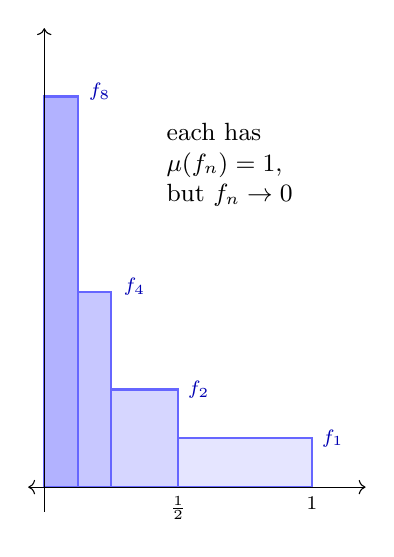
\begin{tikzpicture}[x=3.4cm, y=0.62cm]
	\draw[fill=blue!10, draw=blue!60, thick] (0,0) rectangle (1,1);
	\draw[fill=blue!16, draw=blue!60, thick] (0,0) rectangle (0.5,2);
	\draw[fill=blue!22, draw=blue!60, thick] (0,0) rectangle (0.25,4);
	\draw[fill=blue!30, draw=blue!60, thick] (0,0) rectangle (0.125,8);
	\draw[<->] (-0.06,0) -- (1.2,0);
	\draw[->] (0,-0.5) -- (0,9.4);
	\node[below, font=\scriptsize] at (1,0) {$1$};
	\node[below, font=\scriptsize] at (0.5,0) {$\tfrac12$};
	\node[right, font=\scriptsize, blue!70!black] at (1.0,1.0) {$f_1$};
	\node[right, font=\scriptsize, blue!70!black] at (0.5,2.0) {$f_2$};
	\node[right, font=\scriptsize, blue!70!black] at (0.26,4.1) {$f_4$};
	\node[right, font=\scriptsize, blue!70!black] at (0.13,8.1) {$f_8$};
	\node[font=\small, anchor=west, align=left] at (0.42, 6.6) {each has\\ $\mu(f_n)=1$,\\ but $f_n \to 0$};
\end{tikzpicture}
\end{center}

To rule out escaping mass we need a hypothesis that pins the functions down, and the cheapest one is domination.

\begin{theorem}[Dominated convergence theorem]\label{pm-thm:dct}
	Let $f_n, f$ be measurable with $f_n \to f$ almost everywhere, and suppose there is an integrable $g$ with $|f_n| \leq g$ almost everywhere for every $n$. Then $f_n, f \in L^1(\mu)$ and
	$$
	\mu(f_n) \to \mu(f), \qquad \text{and indeed } \mu(|f_n - f|) \to 0.
	$$
\end{theorem}
\begin{proof}
	Since $|f_n| \leq g$ we get $\mu(|f_n|)\leq \mu(g) < \infty$; letting $n\to\infty$ pointwise gives $|f| \leq g$ a.e., so $f$ is integrable too. Now $|f_n - f| \leq 2g$, so $2g - |f_n - f| \geq 0$, and $2g - |f_n-f| \to 2g$ a.e. By Fatou,
	$$
	\mu(2g) = \mu\big(\liminf_n (2g - |f_n - f|)\big) \leq \liminf_n \mu\big(2g - |f_n-f|\big) = \mu(2g) - \limsup_n \mu(|f_n-f|).
	$$
	As $\mu(2g) < \infty$ we may cancel, giving $\limsup_n \mu(|f_n-f|) \leq 0$. Hence $\mu(|f_n - f|)\to 0$, and $|\mu(f_n)-\mu(f)| \leq \mu(|f_n-f|) \to 0$.
\end{proof}

\begin{example}[Bounded convergence]
	If $\mu(E) < \infty$, $f_n \to f$ pointwise, and $\sup_n\|f_n\|_\infty \leq C < \infty$, then the constant function $C$ is integrable and dominates, so $\mu(f_n)\to\mu(f)$. Note that no uniformity of the convergence is required -- contrast with the Riemann theory, where the standard theorem needs uniform convergence.
\end{example}

\begin{example}
	Compute $\lim_{n\to\infty}\int_0^\infty \big(1+\tfrac{x}{n}\big)^{-n}\sin(x/n)\dd x$. The integrand tends to $0$ pointwise, and for $n \geq 2$ we have $(1+x/n)^{-n}|\sin(x/n)| \leq (1+x/2)^{-2}$, which is integrable on $(0,\infty)$. By dominated convergence the limit is $0$.
\end{example}

\subsection{Comparison with the Riemann integral}

It is reassuring to know that we have not thrown anything away.

\begin{theorem}\label{thm:riemann}
	Let $f : [a,b]\to\R$ be Riemann integrable. Then $f$ is Lebesgue measurable with respect to the completed Borel $\sigma$-algebra, is Lebesgue integrable, and the two integrals agree.
\end{theorem}

We will not give the full proof, but the mechanism is easy to describe. If $f$ is Riemann integrable, choose partitions $P_n$ refining each other with mesh tending to $0$, and let $\ell_n$, $u_n$ be the associated lower and upper step functions, so $\ell_n \leq f \leq u_n$ with $\ell_n \uparrow \ell$ and $u_n \downarrow u$ for some measurable $\ell \leq f \leq u$. The Lebesgue integrals of $\ell_n$ and $u_n$ are exactly the lower and upper Riemann sums, and by monotone (or dominated) convergence they converge to $\mu(\ell)$ and $\mu(u)$. Riemann integrability says these limits agree, so $\mu(u - \ell) = 0$, whence $\ell = f = u$ almost everywhere, and $\mu(f)$ is the common value.

\begin{remark}
	The same argument gives Lebesgue's criterion: a bounded function on $[a,b]$ is Riemann integrable if and only if its set of discontinuities is Lebesgue null. And for a \emph{continuous} $f$ the fundamental theorem of calculus survives unchanged, since its proof uses nothing about the integral beyond $\int_x^{x+h}\dd t = h$ and linearity, both of which hold for the Lebesgue integral. So
	$$
	\underbrace{\int_a^x f(t)\dd t}_{\text{Riemann}} = \underbrace{\int_{[a,x]} f \dd\mu}_{\text{Lebesgue}}
	$$
	for continuous $f$, and all the usual techniques -- substitution, integration by parts -- extend to bounded measurable functions by the monotone class theorem.
\end{remark}

The converse of Theorem \ref{thm:riemann} fails badly: $\ind_\Q$ is Lebesgue integrable but not Riemann integrable. Better still, the Lebesgue theory handles unbounded domains and unbounded functions in a single framework, with no need for the improper-integral gymnastics of Analysis I.

\subsection{Integrals depending on a parameter}

A standard and constantly useful application of dominated convergence.

\begin{theorem}[Continuity and differentiation under the integral]\label{thm:diff-under}
	Let $U \subseteq \R$ be open, let $(E,\cE,\mu)$ be a measure space, and let $f : U \times E \to \R$ be such that $x \mapsto f(t,x)$ is measurable for each $t$. Set $F(t) = \int_E f(t,x)\dd\mu(x)$.
	\begin{enumerate}[label=(\roman*)]
		\item Suppose $t \mapsto f(t,x)$ is continuous for each $x$, and $|f(t,x)| \leq g(x)$ for all $t \in U$ with $g$ integrable. Then $F$ is continuous on $U$.
		\item Suppose $t\mapsto f(t,x)$ is differentiable for each $x$, and $\big|\frac{\partial f}{\partial t}(t,x)\big| \leq g(x)$ for all $t \in U$ with $g$ integrable. Then $F$ is differentiable on $U$ with
		$$
		F'(t) = \int_E \frac{\partial f}{\partial t}(t,x)\dd\mu(x).
		$$
	\end{enumerate}
\end{theorem}
\begin{proof}
	(i) Let $t_n \to t$ in $U$. Then $f(t_n, \cdot) \to f(t,\cdot)$ pointwise, dominated by $g$, so $F(t_n)\to F(t)$ by dominated convergence. Since sequential continuity suffices on $\R$, we are done.

	(ii) Fix $t \in U$ and let $h_n \to 0$ with $h_n \neq 0$. Put
	$$
	g_n(x) = \frac{f(t+h_n,x)-f(t,x)}{h_n} - \frac{\partial f}{\partial t}(t,x).
	$$
	By the mean value theorem there is $\tilde t$ between $t$ and $t+h_n$ with the difference quotient equal to $\frac{\partial f}{\partial t}(\tilde t, x)$, so $|g_n(x)| \leq 2g(x)$, an integrable bound. By differentiability $g_n(x)\to 0$ for each $x$, so by dominated convergence $\mu(g_n)\to 0$. But by linearity
	$$
	\mu(g_n) = \frac{F(t+h_n)-F(t)}{h_n} - \int_E \frac{\partial f}{\partial t}(t,x)\dd\mu(x),
	$$
	which gives the claim.
\end{proof}

\subsection{New measures from old}

Two constructions come up constantly.

\begin{proposition}[Image measures and the change of variables formula]\label{prop:change-var}
	Let $f : (E,\cE,\mu)\to(G,\cG)$ be measurable and $\nu = \mu\circ f^{-1}$. If $g : G \to \R$ is measurable and either non-negative or $\nu$-integrable, then
	$$
	\nu(g) = \int_G g\dd\nu = \int_E g\circ f\dd\mu = \mu(g \circ f).
	$$
\end{proposition}
\begin{proof}
	For $g = \ind_A$ with $A \in \cG$, both sides equal $\mu(f^{-1}(A)) = \nu(A)$. By linearity the identity holds for simple $g$; by monotone convergence along the standard approximation it holds for non-negative measurable $g$; and by splitting $g = g^+-g^-$ it holds in the integrable case.
\end{proof}

Specialising to a random variable $X$ on $(\Omega,\cF,\PP)$ with law $\mu_X$ gives the formula that we used without proof in IA:
$$
\EE[g(X)] = \int_\Omega g(X(\omega))\dd\PP(\omega) = \int_E g(x)\dd\mu_X(x).
$$
In particular, the expectation of $g(X)$ depends only on the law of $X$, which is why in practice one only ever writes down distributions.

\begin{proposition}[Measures with densities]\label{prop:density}
	Let $f : (E,\cE,\mu)\to[0,\infty]$ be measurable and define
	$$
	\nu(A) = \mu(f\ind_A), \qquad A \in \cE.
	$$
	Then $\nu$ is a measure on $(E,\cE)$, and for measurable $g \geq 0$,
	$$
	\nu(g) = \mu(fg).
	$$
	We call $f$ the \vocab{density} of $\nu$ with respect to $\mu$ and write $\dd\nu = f\dd\mu$.
\end{proposition}
\begin{proof}
	$\nu(\varnothing)=0$ is clear, and countable additivity follows from Theorem \ref{thm:int-nonneg}(iv) applied to $\sum_n f\ind_{A_n} = f\ind_{\bigsqcup A_n}$. The identity $\nu(g)=\mu(fg)$ holds for $g$ an indicator by definition, hence for simple $g$ by linearity, hence in general by monotone convergence.
\end{proof}

If $\nu$ is a probability measure we call $f$ a \vocab{probability density function}, and this recovers the continuous random variables of IA Probability: the statement `$X$ has density $f$' means precisely that $\mu_X$ has density $f$ with respect to Lebesgue measure, and then $\EE[g(X)] = \int_\R g(x)f(x)\dd x$.

\section{Product Measures and Fubini's Theorem}

\subsection{Product \texorpdfstring{$\sigma$}{sigma}-algebras and sections}

If we want to integrate functions of two variables -- and we do, since that is how sums of independent random variables work -- we need a measure on a product space.

\begin{definition}[Product $\sigma$-algebra]
	Let $(E_1,\cE_1)$ and $(E_2,\cE_2)$ be measurable spaces. On $E = E_1\times E_2$ let
	$$
	\cA = \{A_1\times A_2 : A_1 \in \cE_1,\; A_2 \in \cE_2\}
	$$
	be the collection of \vocab{measurable rectangles}, a $\pi$-system since $(A_1\times A_2)\cap(B_1\times B_2) = (A_1\cap B_1)\times(A_2\cap B_2)$. The \vocab{product $\sigma$-algebra} is $\cE_1\otimes\cE_2 = \sigma(\cA)$.
\end{definition}

If $E_1, E_2$ are topological spaces with countable bases then $\cB(E_1\times E_2) = \cB(E_1)\otimes\cB(E_2)$; in particular $\cB(\R^2)=\cB\otimes\cB$, and inductively $\cB(\R^d) = \cB^{\otimes d}$.

\begin{lemma}[Sections are measurable]\label{lem:sections}
	Let $f : (E_1\times E_2, \cE_1\otimes\cE_2)\to\R$ be measurable. Then for each fixed $x_1 \in E_1$ the map $x_2 \mapsto f(x_1,x_2)$ is $\cE_2$-measurable.
\end{lemma}
\begin{proof}
	Let $\cV$ be the set of bounded measurable $f$ for which the conclusion holds. This is a vector space; it contains $\ind_E$; and for a rectangle $A = A_1\times A_2$ we have $\ind_A(x_1,x_2) = \ind_{A_1}(x_1)\ind_{A_2}(x_2)$, which as a function of $x_2$ is either $\ind_{A_2}$ or $0$, so $\ind_A \in \cV$. If $0 \leq f_n \uparrow f$ with $f_n \in \cV$ and $f$ bounded, then $x_2\mapsto f(x_1,x_2)$ is a pointwise limit of measurable functions, hence measurable, so $f \in \cV$. By the monotone class theorem (Theorem \ref{thm:mct-class}), $\cV$ contains all bounded measurable functions. For general measurable $f$, apply this to the truncations $(-n)\vee f\wedge n$ and take limits.
\end{proof}

\begin{lemma}[Partial integrals are measurable]\label{lem:partial-int}
	Let $(E_i,\cE_i,\mu_i)$ be finite measure spaces and let $f$ on $E_1\times E_2$ be measurable and either bounded or non-negative. Then
	$$
	x_1 \longmapsto \int_{E_2} f(x_1,x_2)\dd\mu_2(x_2)
	$$
	is $\cE_1$-measurable, and is bounded (resp.\ non-negative) accordingly.
\end{lemma}
\begin{proof}
	Again let $\cV$ be the collection of bounded measurable $f$ for which the conclusion holds. It is a vector space by linearity of the integral. For a rectangle, $\int_{E_2}\ind_{A_1}(x_1)\ind_{A_2}(x_2)\dd\mu_2 = \ind_{A_1}(x_1)\mu_2(A_2)$, which is measurable and bounded by $\mu_2(E_2)<\infty$; likewise $\ind_E \in \cV$. If $0 \leq f_n \uparrow f$ with $f_n \in \cV$ and $f$ bounded, then by monotone convergence
	$$
	\int_{E_2} f(x_1,x_2)\dd\mu_2(x_2) = \lim_n \int_{E_2} f_n(x_1,x_2)\dd\mu_2(x_2)
	$$
	is an increasing limit of measurable functions, hence measurable, and bounded by $\mu_2(E_2)\|f\|_\infty$. So $\cV$ contains all bounded measurable functions. The non-negative case follows by applying this to $f \wedge n$ and using monotone convergence again.
\end{proof}

\subsection{The product measure}

\begin{theorem}[Existence and uniqueness of the product measure]\label{thm:product}
	Let $(E_1,\cE_1,\mu_1)$ and $(E_2,\cE_2,\mu_2)$ be finite measure spaces. There is a unique measure $\mu = \mu_1\otimes\mu_2$ on $(E_1\times E_2, \cE_1\otimes\cE_2)$ with
	$$
	\mu(A_1\times A_2) = \mu_1(A_1)\mu_2(A_2) \qquad \text{for all } A_i \in \cE_i.
	$$
\end{theorem}
\begin{proof}
	Uniqueness is Theorem \ref{pm-thm:uniqueness}: the rectangles form a $\pi$-system generating $\cE_1\otimes\cE_2$ and containing $E$, and the total mass $\mu_1(E_1)\mu_2(E_2)$ is finite.

	For existence, define
	$$
	\mu(A) = \int_{E_1}\Big( \int_{E_2}\ind_A(x_1,x_2)\dd\mu_2(x_2)\Big)\dd\mu_1(x_1),
	$$
	which makes sense by Lemmas \ref{lem:sections} and \ref{lem:partial-int}. On a rectangle,
	$$
	\mu(A_1\times A_2) = \int_{E_1}\ind_{A_1}(x_1)\mu_2(A_2)\dd\mu_1(x_1) = \mu_1(A_1)\mu_2(A_2).
	$$
	Clearly $\mu(\varnothing) = 0$. For countable additivity, let $(A_n)$ be disjoint in $\cE_1\otimes\cE_2$. Then $\ind_{\bigsqcup_n A_n} = \sum_n \ind_{A_n}$, and applying the monotone convergence theorem twice (once in each integral) together with linearity gives
	$$
	\mu\Big(\bigsqcup_n A_n\Big) = \lim_{N}\sum_{n=1}^N \int_{E_1}\int_{E_2}\ind_{A_n}\dd\mu_2\dd\mu_1 = \sum_{n=1}^\infty \mu(A_n). \qedhere
	$$
\end{proof}

\subsection{Fubini's theorem}

\begin{theorem}[Fubini--Tonelli]\label{thm:fubini}
	Let $(E,\cE,\mu) = (E_1\times E_2, \cE_1\otimes\cE_2,\mu_1\otimes\mu_2)$ with $\mu_1,\mu_2$ finite.
	\begin{enumerate}[label=(\roman*)]
		\item \textup{(Tonelli)} If $f : E \to[0,\infty]$ is measurable then
		\begin{align*}
			\int_E f\dd\mu &= \int_{E_1}\Big(\int_{E_2} f(x_1,x_2)\dd\mu_2(x_2)\Big)\dd\mu_1(x_1)\\
			&= \int_{E_2}\Big(\int_{E_1} f(x_1,x_2)\dd\mu_1(x_1)\Big)\dd\mu_2(x_2).
		\end{align*}
		\item \textup{(Fubini)} If $f \in L^1(\mu)$, let
		$$
		A_1 = \Big\{ x_1 \in E_1 : \int_{E_2}|f(x_1,x_2)|\dd\mu_2(x_2)<\infty\Big\}
		$$
		and set $f_1(x_1) = \int_{E_2}f(x_1,x_2)\dd\mu_2(x_2)$ for $x_1 \in A_1$ and $f_1 = 0$ elsewhere. Then $\mu_1(A_1^c) = 0$, $f_1 \in L^1(\mu_1)$, and $\mu(f) = \mu_1(f_1)$. Symmetrically in the other coordinate.
	\end{enumerate}
\end{theorem}
\begin{proof}
	(i) By the construction of $\mu$ in Theorem \ref{thm:product}, the first identity holds for $f = \ind_A$ with $A$ a measurable rectangle, and the second holds by the symmetric construction; the two constructions agree by uniqueness, so both identities hold for indicators of rectangles, and hence -- since the two sides are measures agreeing on a generating $\pi$-system -- for $f = \ind_A$ with $A \in \cE$. By linearity they extend to simple $f$, and by monotone convergence along the standard approximation to all measurable $f \geq 0$.

	(ii) Let $h(x_1) = \int_{E_2}|f(x_1,x_2)|\dd\mu_2(x_2)$. By part (i) applied to $|f|$,
	$$
	\mu_1(h) = \mu(|f|)<\infty,
	$$
	so $h$ is integrable and hence finite $\mu_1$-almost everywhere; that is, $\mu_1(A_1^c)=0$. Applying part (i) to $f^+$ and $f^-$ separately, the functions $f_1^\pm(x_1) = \int_{E_2}f^\pm(x_1,x_2)\dd\mu_2(x_2)$ satisfy $\mu_1(f_1^\pm) = \mu(f^\pm) < \infty$, and $f_1 = f_1^+ - f_1^-$ on $A_1$. Hence
	$$
	\mu(f) = \mu(f^+)-\mu(f^-) = \mu_1(f_1^+)-\mu_1(f_1^-) = \mu_1(f_1). \qedhere
	$$
\end{proof}

\begin{remark}
	The integrability hypothesis in (ii) matters. On $(0,1)^2$ with Lebesgue measure, let
	$$
	f(x,y) = \frac{x^2-y^2}{(x^2+y^2)^2}.
	$$
	One computes $\int_0^1\big(\int_0^1 f\dd y\big)\dd x = \pi/4$ and $\int_0^1\big(\int_0^1 f\dd x\big)\dd y = -\pi/4$. The two iterated integrals disagree, and indeed $\int\int|f| = \infty$, so Fubini does not apply. In practice one always runs Tonelli on $|f|$ first to check integrability, and only then applies Fubini to $f$.
\end{remark}

\begin{remark}[$\sigma$-finite measures and higher dimensions]
	Everything above extends to $\sigma$-finite $\mu_i$ by exhausting $E_i$ with sets of finite measure and taking limits. Moreover $(\cE_1\otimes\cE_2)\otimes\cE_3 = \cE_1\otimes(\cE_2\otimes\cE_3)$, by a $\pi$-system argument, so the construction iterates: there is a unique measure $\mu_1\otimes\cdots\otimes\mu_n$ on $\prod_i E_i$ with
	$$
	(\mu_1\otimes\cdots\otimes\mu_n)(A_1\times\cdots\times A_n)=\prod_i \mu_i(A_i).
	$$
	In particular, taking each $\mu_i$ to be Lebesgue measure on $\R$, we obtain \vocab{Lebesgue measure on $\R^d$}: the unique Borel measure with
	$$
	\mu^d\Big(\prod_{i=1}^d (a_i,b_i]\Big) = \prod_{i=1}^d (b_i-a_i).
	$$
	It is translation invariant, and Fubini says that integration over $\R^d$ may be performed one coordinate at a time in any order, for non-negative or integrable $f$.
\end{remark}

\subsection{Product probability spaces and independence}

Fubini gives the clean measure-theoretic statement of independence.

\begin{proposition}\label{prop:indep-product}
	Let $X = (X_1,\dots,X_n) : (\Omega,\cF,\PP)\to \big(\prod_i E_i, \bigotimes_i \cE_i\big)$ be measurable. The following are equivalent:
	\begin{enumerate}[label=(\roman*)]
		\item $X_1,\dots,X_n$ are independent;
		\item $\mu_X = \bigotimes_{i=1}^n \mu_{X_i}$;
		\item for all bounded measurable $f_i : E_i \to \R$, $\;\EE\big[\prod_i f_i(X_i)\big] = \prod_i \EE[f_i(X_i)]$.
	\end{enumerate}
\end{proposition}
\begin{proof}
	(i)$\Rightarrow$(ii). On the $\pi$-system of rectangles,
	$$
	\mu_X\Big(\prod_i A_i\Big) = \PP(X_1\in A_1,\dots,X_n\in A_n)=\prod_i \PP(X_i\in A_i) = \Big(\bigotimes_i\mu_{X_i}\Big)\Big(\prod_i A_i\Big),
	$$
	so the two probability measures agree by uniqueness of extension.

	(ii)$\Rightarrow$(iii). By the change of variables formula and Fubini (the integrand is bounded, hence integrable for a probability measure),
	$$
	\EE\Big[\prod_i f_i(X_i)\Big] = \int \prod_i f_i(x_i)\dd\Big(\bigotimes_i\mu_{X_i}\Big)(x) = \prod_i \int_{E_i} f_i\dd\mu_{X_i} = \prod_i \EE[f_i(X_i)].
	$$

	(iii)$\Rightarrow$(i). Take $f_i = \ind_{A_i}$.
\end{proof}

\begin{example}[Densities of sums]
	Let $X,Y$ be independent real random variables with densities $f,g$. By Fubini, for $A \in \cB$,
	$$
	\PP(X+Y\in A) = \int_{\R^2}\ind_A(x+y)f(x)g(y)\dd x\dd y = \int_\R \ind_A(v)\Big(\int_\R f(v-y)g(y)\dd y\Big)\dd v,
	$$
	substituting $v = x+y$ and using translation invariance. So $X+Y$ has density the convolution $f * g$. This recovers, and now justifies, the formula from IA Probability.
\end{example}
\section{Norms and Inequalities}

\subsection{\texorpdfstring{$L^p$}{Lp} spaces}

Having built the integral we can build function spaces out of it, and this is where measure theory starts to look like analysis again. Recall from IB Analysis and Topology that a \vocab{norm} on a real vector space $V$ is a map $\|\cdot\| : V \to [0,\infty)$ with $\|\lambda v\| = |\lambda|\|v\|$, $\|u+v\|\leq\|u\|+\|v\|$, and $\|v\|=0$ only for $v=0$.

\begin{definition}[$L^p$ spaces]
	Let $(E,\cE,\mu)$ be a measure space and $1 \leq p \leq \infty$. For measurable $f : E \to \R$ put
	$$
	\|f\|_p = \begin{cases}
		\Big( \int_E |f|^p \dd\mu\Big)^{1/p}, & 1 \leq p < \infty,\\[4pt]
		\esssup |f| = \inf\{\lambda \geq 0 : |f| \leq \lambda \text{ a.e.}\}, & p = \infty,
	\end{cases}
	$$
	and let $L^p = L^p(E,\cE,\mu)$ be the set of measurable $f$ with $\|f\|_p < \infty$.
\end{definition}

There is one wrinkle. If $\|f\|_p = 0$ then $|f|^p = 0$ almost everywhere, so $f = 0$ almost everywhere -- but $f$ need not be identically zero. So $\|\cdot\|_p$ is only a seminorm on $L^p$. The standard fix is to quotient out:

\begin{definition}
	Write $f \sim g$ if $f = g$ $\mu$-almost everywhere. This is an equivalence relation, and we write $\cL^p = L^p/\!\sim$ for the space of equivalence classes. Then $\|\cdot\|_p$ is a genuine norm on $\cL^p$.
\end{definition}

In practice everyone abuses notation and talks about `the function $f \in \cL^p$', meaning a representative of its class; no confusion arises, because every operation we perform is insensitive to modification on a null set. We will do the same.

Homogeneity of $\|\cdot\|_p$ is clear, and the triangle inequality is easy for $p=1$ (integrate $|f+g|\leq|f|+|g|$) and for $p=\infty$. For $1<p<\infty$ it is Minkowski's inequality, which we prove below via H\"older. Before that, two inequalities that need no such machinery.

\subsection{Markov, Chebyshev and Jensen}

\begin{proposition}[Markov's inequality]\label{prop:markov}
	Let $f : E \to[0,\infty]$ be measurable. Then for every $\lambda>0$,
	$$
	\mu(\{f \geq \lambda\}) \leq \frac{\mu(f)}{\lambda}.
	$$
\end{proposition}
\begin{proof}
	Integrate the pointwise inequality $\lambda\ind_{\{f\geq\lambda\}} \leq f$.
\end{proof}

That is the whole proof, and yet it is the workhorse of the subject: it converts information about an average into information about a tail.

\begin{corollary}[Chebyshev's inequality]
	If $X$ is a random variable with $\EE[X^2] < \infty$ then for $\lambda>0$,
	$$
	\PP\big( |X - \EE[X]| \geq \lambda\big) \leq \frac{\var(X)}{\lambda^2}.
	$$
	More generally, $\PP(|X| \geq \lambda) \leq \lambda^{-p}\EE[|X|^p]$ for any $p > 0$.
\end{corollary}
\begin{proof}
	Apply Markov to $|X - \EE X|^2$, respectively $|X|^p$, with threshold $\lambda^2$ respectively $\lambda^p$.
\end{proof}

Next, convexity. Recall that $c : I \to \R$ on an interval $I$ is \vocab{convex} if
$$
c(tx + (1-t)y) \leq tc(x)+(1-t)c(y) \qquad (x,y \in I,\; t\in[0,1]),
$$
equivalently if the slopes $\frac{c(t)-c(x)}{t-x}$ are non-decreasing in each argument. A convex function is continuous on $I^\circ$, hence Borel measurable.

\begin{lemma}[Supporting line]\label{lem:support}
	Let $c$ be convex on $I$ and let $m \in I^\circ$. Then there are $a,b\in\R$ with $c(x) \geq ax+b$ for all $x \in I$ and $c(m)=am+b$.
\end{lemma}
\begin{proof}
	Let
	$$
	a = \sup\Big\{ \frac{c(m)-c(x)}{m-x} : x \in I, \; x<m\Big\},
	$$
	which is finite by the slope characterisation of convexity (the slopes to the left of $m$ are bounded above by any slope to the right). Set $b = c(m)-am$. For $y>m$ we have $a \leq \frac{c(y)-c(m)}{y-m}$, so $c(y)\geq ay+b$; for $y<m$, by definition of the supremum $\frac{c(m)-c(y)}{m-y}\leq a$, which rearranges to $c(y)\geq ay+b$ again.
\end{proof}

\begin{center}
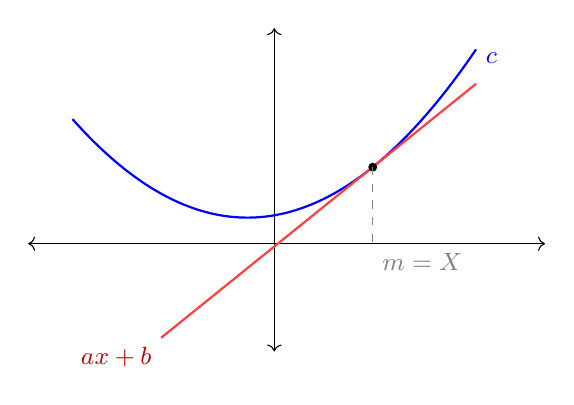
\begin{tikzpicture}[x=1.25cm,y=0.72cm]
	\draw[<->] (-2.5,0) -- (2.75,0);
	\draw[<->] (0,-1.9) -- (0,3.8);
	\draw[thick, smooth, samples=100, domain=-2.05:2.05, color=blue] plot (\x, {0.55*\x*\x + 0.3*\x + 0.5});
	% supporting line at m=1: c(1)=1.35, c'(1)=1.1*1+0.3=1.4 -> y = 1.4x - 0.05
	\draw[thick, red!75, domain=-1.15:2.05] plot (\x, {1.4*\x - 0.05});
	\fill (1, 1.35) circle (1.6pt);
	\draw[dashed, gray] (1,1.35) -- (1,0);
	\node[below right, font=\small, gray] at (1,0) {$m=\EE X$};
	\node[blue, anchor=west, font=\small] at (2.05, 3.28) {$c$};
	\node[red!75!black, anchor=north east, font=\small] at (-1.15,-1.66) {$ax+b$};
\end{tikzpicture}
\end{center}

\begin{theorem}[Jensen's inequality]\label{thm:jensen}
	Let $X$ be a random variable taking values in an interval $I$ with $\EE|X| < \infty$, and let $c : I \to \R$ be convex. Then $\EE[c(X)]$ is well defined in $(-\infty,\infty]$ and
	$$
	c\big(\EE[X]\big) \leq \EE\big[c(X)\big].
	$$
\end{theorem}
\begin{proof}
	Let $m = \EE[X] \in I$. If $m \notin I^\circ$ then $m$ is an endpoint of $I$ and $X = m$ almost surely (a non-degenerate random variable on $I$ has mean in the interior), so both sides are $c(m)$.

	Otherwise take $a,b$ as in Lemma \ref{lem:support}, so $c(x) \geq ax + b$ on $I$. Then $c^-(X) \leq |a||X| + |b|$, so $\EE[c^-(X)] < \infty$ and $\EE[c(X)] = \EE[c^+(X)]-\EE[c^-(X)]$ is well defined in $(-\infty,\infty]$. Integrating $c(X)\geq aX+b$,
	$$
	\EE[c(X)] \geq a\EE[X]+b = am+b = c(m) = c(\EE[X]). \qedhere
	$$
\end{proof}

\begin{corollary}[Monotonicity of $L^p$ norms on probability spaces]\label{cor:lp-nested}
	Let $1 \leq p \leq q \leq \infty$. Then $\|X\|_p \leq \|X\|_q$ for any random variable $X$ on a probability space, and hence $\cL^q(\PP)\subseteq\cL^p(\PP)$.
\end{corollary}
\begin{proof}
	The case $q = \infty$ is clear. For $q<\infty$, the map $c(x) = |x|^{q/p}$ is convex since $q/p \geq 1$. Applying Jensen to the random variable $|X|^p$ (assume first that $X$ is bounded, so all expectations are finite),
	$$
	\big(\EE|X|^p\big)^{q/p} = c\big(\EE|X|^p\big) \leq \EE\big[c(|X|^p)\big] = \EE|X|^q,
	$$
	so $\|X\|_p \leq \|X\|_q$. For general $X \in \cL^q$, apply this to $|X|\wedge n$ and let $n \to\infty$ using monotone convergence.
\end{proof}

This is a genuinely probabilistic phenomenon: it uses $\PP(\Omega)=1$ crucially, and fails for infinite measure spaces, as we will see.

\subsection{H\"older and Minkowski}

\begin{definition}
	We call $p,q \in[1,\infty]$ \vocab{conjugate exponents} if $\frac1p+\frac1q=1$, with the convention $\frac1\infty = 0$.
\end{definition}

\begin{theorem}[H\"older's inequality]\label{pm-thm:holder}
	Let $p,q$ be conjugate and let $f,g$ be measurable on $(E,\cE,\mu)$. Then
	$$
	\mu(|fg|) \leq \|f\|_p\|g\|_q.
	$$
\end{theorem}
\begin{proof}
	If $p=1$, $q=\infty$: $|fg|\leq |f|\,\|g\|_\infty$ almost everywhere, and integrate. Symmetrically for $p = \infty$. So assume $1<p<\infty$.

	We may assume $\|f\|_p, \|g\|_q < \infty$, else the right side is infinite. We may also assume $\|f\|_p > 0$ (else $f = 0$ a.e.\ and both sides vanish), and by homogeneity we may rescale so that $\|f\|_p = 1$.

	The point is that $\dd\PP = |f|^p\dd\mu$ is then a probability measure. Writing
	$$
	\mu(|fg|) = \int_E \frac{|g|}{|f|^{p-1}}\,\ind_{\{|f|>0\}}\,|f|^p\dd\mu = \int_E \frac{|g|}{|f|^{p-1}}\ind_{\{|f|>0\}}\dd\PP,
	$$
	we may apply Corollary \ref{cor:lp-nested} with exponents $1 \leq q$ on the probability space $(E,\cE,\PP)$:
	$$
	\int \frac{|g|}{|f|^{p-1}}\ind_{\{|f|>0\}}\dd\PP \leq \Big( \int \frac{|g|^q}{|f|^{q(p-1)}}\ind_{\{|f|>0\}}\dd\PP\Big)^{1/q} = \Big( \int_E |g|^q \ind_{\{|f|>0\}}\dd\mu\Big)^{1/q}\!\! \leq \|g\|_q,
	$$
	where we used $q(p-1) = p$, so that $|f|^{-q(p-1)}|f|^p = 1$ on $\{|f|>0\}$. This is the claim, since $\|f\|_p=1$.
\end{proof}

\begin{remark}
	For $p = q = 2$ this is the Cauchy--Schwarz inequality $\mu(|fg|) \leq \|f\|_2\|g\|_2$, which the reader has met in several guises already.
\end{remark}

\begin{theorem}[Minkowski's inequality]\label{pm-thm:minkowski}
	For $1\leq p\leq\infty$ and measurable $f,g$,
	$$
	\|f+g\|_p \leq \|f\|_p+\|g\|_p.
	$$
\end{theorem}
\begin{proof}
	The cases $p=1,\infty$ are immediate. Let $1<p<\infty$ and assume $f,g \in L^p$. First, $|f+g|^p \leq 2^p(|f|^p+|g|^p)$ pointwise, so $f + g \in L^p$; and we may assume $\|f+g\|_p>0$. Let $q$ be conjugate to $p$, so $q(p-1)=p$. Then by the triangle inequality and H\"older,
	\begin{align*}
		\|f+g\|_p^p &= \int_E |f+g|^{p-1}|f+g|\dd\mu \\
		&\leq \int_E |f+g|^{p-1}|f|\dd\mu + \int_E |f+g|^{p-1}|g|\dd\mu\\
		&\leq \Big(\int_E |f+g|^{q(p-1)}\dd\mu\Big)^{1/q}\big(\|f\|_p+\|g\|_p\big)\\
		&= \|f+g\|_p^{p/q}\big(\|f\|_p+\|g\|_p\big).
	\end{align*}
	Dividing by $\|f+g\|_p^{p/q}$ and using $p - p/q = 1$ gives the result.
\end{proof}

So $(\cL^p, \|\cdot\|_p)$ is a normed vector space for every $1 \leq p \leq \infty$.

\begin{example}[Containments and their failure]\label{ex:lp-containment}
	On a probability space we have $\cL^\infty \subseteq \cL^q \subseteq \cL^p \subseteq \cL^1$ for $1\leq p\leq q\leq\infty$, by Corollary \ref{cor:lp-nested}. The same holds on any finite measure space, after rescaling. On $(\R,\cB,\mu)$ with $\mu$ Lebesgue measure, however, \emph{no} containment holds in either direction:
	$$
	f(x) = x^{-1/2}\ind_{(0,1)}(x) \in \cL^1\setminus \cL^2, \qquad g(x) = x^{-1}\ind_{(1,\infty)}(x)\in\cL^2\setminus\cL^1.
	$$
	The first function is too singular at the origin for $\cL^2$; the second has too fat a tail for $\cL^1$. On a finite measure space the second failure mode is unavailable, which is exactly why the containments hold there.
\end{example}

\begin{center}
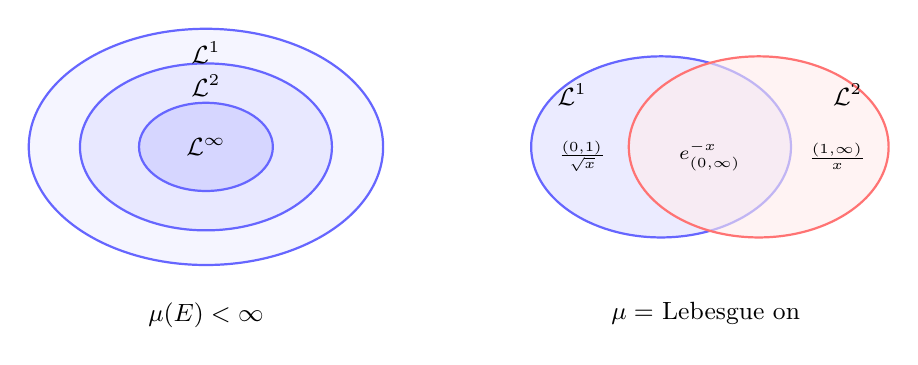
\begin{tikzpicture}
	% Left: finite measure - nested
	\begin{scope}
		\draw[thick, blue!60, fill=blue!4] (0,0) ellipse (2.25 and 1.5);
		\draw[thick, blue!60, fill=blue!9] (0,0) ellipse (1.6 and 1.06);
		\draw[thick, blue!60, fill=blue!16] (0,0) ellipse (0.85 and 0.56);
		\node[font=\small] at (0,0) {$\cL^\infty$};
		\node[font=\small] at (0,0.78) {$\cL^2$};
		\node[font=\small] at (0,1.2) {$\cL^1$};
		\node[font=\small, below] at (0,-1.85) {$\mu(E)<\infty$};
	\end{scope}
	% Right: infinite measure - overlapping
	\begin{scope}[xshift=6.4cm]
		\draw[thick, blue!60, fill=blue!8] (-0.62,0) ellipse (1.65 and 1.15);
		\draw[thick, red!55, fill=red!8, fill opacity=0.6] (0.62,0) ellipse (1.65 and 1.15);
		\node[font=\small] at (-1.75,0.66) {$\cL^1$};
		\node[font=\small] at (1.75,0.66) {$\cL^2$};
		\node[font=\scriptsize] at (-1.62,-0.12) {$\frac{\ind_{(0,1)}}{\sqrt x}$};
		\node[font=\scriptsize] at (1.62,-0.12) {$\frac{\ind_{(1,\infty)}}{x}$};
		\node[font=\scriptsize] at (0,-0.12) {$e^{-x}\ind_{(0,\infty)}$};
		\node[font=\small, below] at (0,-1.85) {$\mu = $ Lebesgue on $\R$};
	\end{scope}
\end{tikzpicture}
\end{center}

\subsection{Completeness}

The great advantage of $\cL^p$ over the space of Riemann integrable functions is that it is complete. Recall that a \vocab{Banach space} is a complete normed vector space.

\begin{theorem}[Riesz--Fischer]\label{thm:riesz-fischer}
	For $1 \leq p\leq\infty$, the space $\cL^p(\mu)$ is a Banach space.
\end{theorem}
\begin{proof}
	The case $p=\infty$ is straightforward (a Cauchy sequence in $\esssup$ is uniformly Cauchy off a null set), so let $1\leq p<\infty$ and let $(f_n)$ be Cauchy in $\cL^p$.

	Extract a subsequence $(f_{N_k})$ with $\|f_{N_{k+1}}-f_{N_k}\|_p \leq 2^{-k}$, so that
	$$
	S = \sum_{k=1}^\infty \|f_{N_{k+1}}-f_{N_k}\|_p \leq 1 < \infty.
	$$
	By Minkowski, for every $K$,
	$$
	\Big\| \sum_{k=1}^K |f_{N_{k+1}}-f_{N_k}| \Big\|_p \leq S,
	$$
	and letting $K \to \infty$ with the monotone convergence theorem (applied to the $p$-th powers, which increase),
	$$
	\Big\| \sum_{k=1}^\infty |f_{N_{k+1}}-f_{N_k}| \Big\|_p \leq S < \infty.
	$$
	In particular $\sum_k |f_{N_{k+1}}-f_{N_k}|$ is finite almost everywhere. On the set $A$ where it is finite -- which has full measure -- the telescoping series
	$$
	f_{N_1} + \sum_{k=1}^\infty (f_{N_{k+1}}-f_{N_k})
	$$
	converges absolutely, so $f_{N_k}(x)$ converges for $x \in A$ by completeness of $\R$. Define $f = \lim_k f_{N_k}$ on $A$ and $f = 0$ off $A$; then $f$ is measurable and $f_{N_k}\to f$ almost everywhere.

	Finally, fix $\varepsilon>0$ and take $N$ with $\|f_n - f_m\|_p \leq \varepsilon$ for $n,m\geq N$. For $n \geq N$, Fatou's lemma gives
	$$
	\|f_n - f\|_p^p = \mu\big(\lim_k |f_n - f_{N_k}|^p\big) \leq \liminf_k \mu\big(|f_n-f_{N_k}|^p\big) \leq \varepsilon^p.
	$$
	So $f_n - f \in \cL^p$, hence $f \in \cL^p$, and $\|f_n-f\|_p \to 0$.
\end{proof}

\begin{remark}
	The proof shows a little more: a sequence converging in $\cL^p$ has a subsequence converging almost everywhere. We will use this repeatedly.
\end{remark}

\begin{remark}[Dense subspaces]
	Each of
	$$
	C([a,b]), \qquad \{\text{simple functions}\}, \qquad \{\text{linear combinations of indicators of intervals}\}
	$$
	is dense in $\cL^1([a,b])$ for Lebesgue measure. So $\cL^1$ is precisely the completion of the continuous functions in the $\|\cdot\|_1$ norm -- which is a far more satisfying description of `the integrable functions' than anything the Riemann theory offers, and is the reason completeness matters.
\end{remark}

\subsection{\texorpdfstring{$\cL^2$}{L2} as a Hilbert space}

When $p=2$ there is extra structure.

\begin{definition}[Hilbert space]
	An \vocab{inner product} on a real vector space $V$ is a symmetric bilinear form $\ip{\cdot}{\cdot}$ with $\ip{v}{v} \geq 0$ and $\ip{v}{v}=0$ only for $v = 0$. It induces a norm $\|v\|=\sqrt{\ip{v}{v}}$. A \vocab{Hilbert space} is an inner product space complete for this norm.
\end{definition}

\begin{corollary}
	$\cL^2(\mu)$ is a Hilbert space with $\ip{f}{g} = \int_E fg\dd\mu$.
\end{corollary}
\begin{proof}
	The integral defining $\ip{f}{g}$ converges by Cauchy--Schwarz, and the form is clearly symmetric and bilinear with $\ip{f}{f}=\|f\|_2^2$. Completeness is Theorem \ref{thm:riesz-fischer}.
\end{proof}

Two identities follow by expanding, and are worth recording.

\begin{lemma}
	For $f,g\in\cL^2$:
	$$
	\|f+g\|_2^2 = \|f\|_2^2 + 2\ip{f}{g}+\|g\|_2^2 \quad \textup{(Pythagoras)},
	$$
	$$
	\|f+g\|_2^2 + \|f-g\|_2^2 = 2\big(\|f\|_2^2+\|g\|_2^2\big) \quad \textup{(parallelogram law)}.
	$$
\end{lemma}

We say $f$ and $g$ are \vocab{orthogonal}, written $f \perp g$, if $\ip{f}{g}=0$; by Pythagoras this happens iff $\|f+g\|_2^2=\|f\|_2^2+\|g\|_2^2$.

\begin{example}[The probabilistic dictionary]
	On a probability space, for $X,Y \in \cL^2(\PP)$ with means $m_X, m_Y$,
	$$
	\var(X) = \|X - m_X\|_2^2, \qquad \cov(X,Y) = \ip{X-m_X}{Y-m_Y}.
	$$
	So variance is squared distance from the mean, and uncorrelatedness is orthogonality of the centred variables. The Cauchy--Schwarz inequality becomes $|\cov(X,Y)|\leq\sqrt{\var X \var Y}$, and Pythagoras becomes the additivity of variance for uncorrelated variables.
\end{example}

\begin{definition}
	For $V\subseteq \cL^2(\mu)$ let $V^\perp = \{f \in \cL^2 : \ip{f}{g} = 0 \text{ for all } g \in V\}$. We call a subspace $V \subseteq \cL^2$ \vocab{closed} if whenever $f_n \in V$ with $f_n \to f$ in $\cL^2$, there is $v \in V$ with $v = f$ almost everywhere.
\end{definition}

\begin{theorem}[Orthogonal projection]\label{thm:projection}
	Let $V$ be a closed subspace of $\cL^2(\mu)$. Then every $f \in \cL^2$ has a decomposition
	$$
	f = v + u, \qquad v \in V, \; u \in V^\perp,
	$$
	unique up to null sets, and $v$ is the unique closest point of $V$ to $f$:
	$$
	\|f - v\|_2 \leq \|f-g\|_2 \quad \text{for all } g \in V,
	$$
	with equality only if $g = v$ a.e. We write $v = P_V f$.
\end{theorem}
\begin{proof}
	Let $d = d(f,V) = \inf_{g \in V}\|f-g\|_2$ and choose $g_n \in V$ with $\|f - g_n\|_2 \to d$. We first show $(g_n)$ is Cauchy. By the parallelogram law applied to $f - g_n$ and $f-g_m$,
	$$
	\|g_n - g_m\|_2^2 = 2\|f-g_n\|_2^2 + 2\|f-g_m\|_2^2 - 4\Big\| f - \frac{g_n+g_m}{2}\Big\|_2^2.
	$$
	Since $\frac{g_n+g_m}{2}\in V$, the last term is at least $4d^2$, so
	$$
	\|g_n-g_m\|_2^2 \leq 2\|f-g_n\|_2^2+2\|f-g_m\|_2^2 - 4d^2 \longrightarrow 0
	$$
	as $n,m\to\infty$. By completeness $g_n \to g$ in $\cL^2$ for some $g$, and since $V$ is closed there is $v \in V$ with $v = g$ a.e. Then $\|f-v\|_2 = \lim_n\|f-g_n\|_2 = d$, so the infimum is attained at $v$.

	Now set $u = f - v$ and let $h \in V$, $t\in\R$. Since $v + th\in V$,
	$$
	d^2 \leq \|f - (v+th)\|_2^2 = d^2 - 2t\ip{u}{h}+t^2\|h\|_2^2,
	$$
	a quadratic in $t$ minimised at $t=0$; differentiating at $t=0$ gives $\ip{u}{h}=0$. As $h \in V$ was arbitrary, $u \in V^\perp$.

	For uniqueness, if also $f = w+z$ with $w\in V$, $z\in V^\perp$, then $(v-w)+(u-z)=0$ with $v - w \in V$ and $u-z\in V^\perp$, so by Pythagoras $0 = \|v-w\|_2^2+\|u-z\|_2^2$, giving $v=w$ and $u=z$ almost everywhere.
\end{proof}

\subsection{Conditional expectation}

We can now give the definition of conditional expectation that makes it a genuine mathematical object rather than a heuristic. The idea is: $\cG \subseteq \cF$ is a sub-$\sigma$-algebra representing partial information, and $\EE[X\mid\cG]$ should be the best prediction of $X$ using only that information. In $\cL^2$, `best prediction' means `nearest point', and that is orthogonal projection.

Let us start with the discrete case, which is the one from IA. Suppose $(G_n)_{n\in\N}$ are disjoint events with $\bigcup_n G_n = \Omega$ and $\PP(G_n) > 0$, and put $\cG = \sigma(G_n : n \in \N)$.

\begin{definition}[Conditional expectation, discrete case]
	For $X \in \cL^1(\PP)$ define
	$$
	\EE[X \mid \cG] = \sum_{n=1}^\infty \EE[X\mid G_n]\ind_{G_n}, \qquad \EE[X\mid G_n] = \frac{\EE[X\ind_{G_n}]}{\PP(G_n)}.
	$$
\end{definition}

So $\EE[X\mid\cG]$ is the random variable which, on the event $G_n$, takes the value of the average of $X$ over $G_n$. It is $\cG$-measurable by construction: it is constant on each atom of $\cG$.

\begin{proposition}\label{prop:cond-exp-proj}
	Let $X \in \cL^2(\PP)$ and let $\cG$ be as above. Then $Y = \EE[X\mid\cG]$ is the orthogonal projection of $X$ onto the closed subspace
	$$
	\cL^2(\cG,\PP) = \{ W \in \cL^2(\PP) : W \text{ is } \cG\text{-measurable}\}.
	$$
\end{proposition}
\begin{proof}
	Any $\cG$-measurable $W$ is constant on each $G_n$, so $W = \sum_n a_n \ind_{G_n}$ for some $a_n \in \R$. Then
	$$
	\EE\big[(X-W)^2\big] = \EE\Big[\sum_n (X-a_n)^2\ind_{G_n}\Big] = \sum_n \PP(G_n)\Big( \EE[X^2\mid G_n] - 2a_n\EE[X\mid G_n]+a_n^2\Big).
	$$
	Each summand is a quadratic in $a_n$ minimised at $a_n = \EE[X\mid G_n]$, independently of the others. Hence $\EE[(X-W)^2]$ is minimised over $\cL^2(\cG,\PP)$ precisely at $W = Y$, and by Theorem \ref{thm:projection} the minimiser is the orthogonal projection.
\end{proof}

\begin{center}
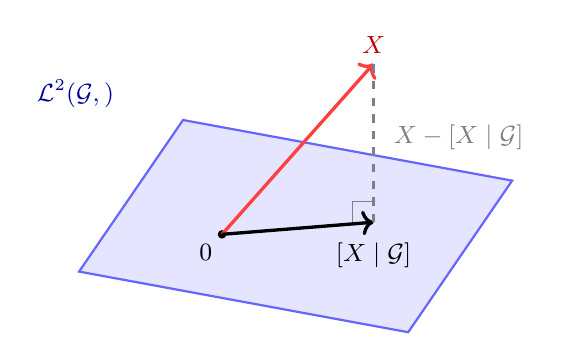
\begin{tikzpicture}[scale=1.1]
	% subspace as a parallelogram
	\fill[blue!10] (-2.4,-0.55) -- (1.4,-1.25) -- (2.6,0.5) -- (-1.2,1.2) -- cycle;
	\draw[blue!60, thick] (-2.4,-0.55) -- (1.4,-1.25) -- (2.6,0.5) -- (-1.2,1.2) -- cycle;
	\node[blue!60!black, font=\small, anchor=west] at (-3.0,1.5) {$\cL^2(\cG,\PP)$};
	% origin
	\coordinate (O) at (-0.75,-0.12);
	\coordinate (V) at (1.0,0.02);
	\coordinate (F) at (1.0,1.85);
	\fill (O) circle (1.4pt);
	\node[below left, font=\small] at (O) {$0$};
	\draw[->, very thick, red!75] (O) -- (F);
	\draw[->, very thick] (O) -- (V);
	\draw[dashed, thick, gray] (V) -- (F);
	% right angle mark
	\draw[gray] ($(V)+(0,0.24)$) -- ($(V)+(-0.24,0.24)$) -- ($(V)+(-0.24,0)$);
	\node[red!75!black, above, font=\small] at (F) {$X$};
	\node[anchor=north, font=\small] at ($(V)+(0,-0.12)$) {$\EE[X\mid\cG]$};
	\node[gray, anchor=west, font=\small] at (1.12,1.0) {$X - \EE[X\mid\cG]$};
\end{tikzpicture}
\end{center}

The picture is the whole content of the definition: $\EE[X\mid\cG]$ is the foot of the perpendicular from $X$ to the subspace of $\cG$-measurable functions. Everything one expects of conditional expectation can be read off from it.

\begin{definition}[Conditional expectation, general case]
	Let $\cG \subseteq \cF$ be a sub-$\sigma$-algebra. For $X \in \cL^2(\PP)$ define $\EE[X\mid\cG] = P_{\cL^2(\cG,\PP)}X$, the orthogonal projection onto the (closed) subspace of $\cG$-measurable square-integrable random variables.
\end{definition}

That $\cL^2(\cG,\PP)$ is closed is exactly the remark after Theorem \ref{thm:riesz-fischer}: a sequence converging in $\cL^2$ has an a.e.\ convergent subsequence, and an a.e.\ limit of $\cG$-measurable functions is $\cG$-measurable.

\begin{proposition}[Characterisation and basic properties]\label{prop:cond-props}
	Let $X \in \cL^2(\PP)$ and $Y = \EE[X\mid\cG]$. Then $Y$ is the a.s.-unique $\cG$-measurable element of $\cL^2$ with
	\begin{equation}\label{eq:cond-defining}
		\EE[Y \ind_A] = \EE[X\ind_A] \qquad \text{for all } A \in \cG. \tag{$\ast$}
	\end{equation}
	Consequently $\EE[Y]=\EE[X]$, the map $X \mapsto \EE[X\mid\cG]$ is linear and monotone, and $\|\EE[X\mid\cG]\|_1 \leq \|X\|_1$.
\end{proposition}
\begin{proof}
	Orthogonality says $\ip{X-Y}{W}=0$ for all $\cG$-measurable $W \in \cL^2$; taking $W = \ind_A$ for $A \in \cG$ (which is bounded, hence in $\cL^2(\PP)$) gives \eqref{eq:cond-defining}. Conversely if $Y'$ is $\cG$-measurable and satisfies \eqref{eq:cond-defining} then $\ip{X-Y'}{\ind_A}=0$ for $A \in \cG$, hence by linearity and monotone class $\ip{X-Y'}{W}=0$ for all bounded $\cG$-measurable $W$, and by approximation for all $W \in \cL^2(\cG,\PP)$; so $Y'=P_{\cL^2(\cG)}X = Y$ a.s.

	Taking $A = \Omega$ in \eqref{eq:cond-defining} gives $\EE Y = \EE X$. Linearity is linearity of projection. For monotonicity, if $X \geq 0$, take $A = \{Y<0\} \in \cG$: then $\EE[Y\ind_A] = \EE[X\ind_A]\geq 0$, and $Y\ind_A \leq 0$, so $Y\ind_A = 0$ a.s.\ and $\PP(A)=0$. Finally, applying monotonicity to $\pm X \leq |X|$ gives $|Y| \leq \EE[|X| \mid \cG]$ a.s., so $\EE|Y| \leq \EE\big[\EE[|X|\mid\cG]\big] = \EE|X|$.
\end{proof}

The $\cL^1$ contraction property in the last line is what lets us extend the definition beyond $\cL^2$.

\begin{theorem}[Extension to $\cL^1$]\label{thm:cond-l1}
	The map $X \mapsto \EE[X\mid\cG]$ extends uniquely from $\cL^2(\PP)$ to a linear contraction $\cL^1(\PP)\to\cL^1(\PP)$, and the extension is still characterised by \eqref{eq:cond-defining}.
\end{theorem}
\begin{proof}
	$\cL^2(\PP)$ is dense in $\cL^1(\PP)$: given $X \in \cL^1$, the truncations $X_n = (-n)\vee X\wedge n$ are bounded, hence in $\cL^2$, and $\|X_n - X\|_1 \to 0$ by dominated convergence. By Proposition \ref{prop:cond-props} the map is a contraction for $\|\cdot\|_1$ on the dense subspace $\cL^2$, and $\cL^1$ is complete, so it extends uniquely by continuity. The identity \eqref{eq:cond-defining} passes to the limit since $|\EE[(X_n - X)\ind_A]| \leq \|X_n - X\|_1$.
\end{proof}

\begin{remark}
	One can also prove existence directly in $\cL^1$ via the Radon--Nikodym theorem, and that is the route usually taken in a course on martingales. The $\cL^2$ route taken here is more elementary and, I think, more illuminating: it makes it clear that conditional expectation is \emph{geometry}, not a formula.
\end{remark}

\begin{example}[Two extremes]
	If $\cG = \{\varnothing,\Omega\}$ then the only $\cG$-measurable functions are constants, and projecting onto the constants gives $\EE[X\mid\cG]=\EE[X]$. If $\cG = \cF$ then $X$ itself is $\cG$-measurable and $\EE[X\mid\cF]=X$. In general $\EE[X\mid\cG]$ interpolates between knowing nothing and knowing everything.
\end{example}
\section{Modes of Convergence}

\subsection{The four modes}

We have met several notions of convergence for random variables, and it is time to organise them.

\begin{definition}
	Let $X_n, X$ be random variables on $(\Omega,\cF,\PP)$.
	\begin{enumerate}[label=(\roman*)]
		\item $X_n \to X$ \vocab{almost surely} if $\PP(X_n \to X) = 1$.
		\item $X_n \to X$ \vocab{in probability}, written $X_n \xrightarrow{\PP}X$, if $\PP(|X_n - X|>\varepsilon)\to 0$ for every $\varepsilon>0$.
		\item $X_n \to X$ \vocab{in $\cL^p$} if $X_n, X \in \cL^p$ and $\|X_n - X\|_p \to 0$.
		\item $X_n \to X$ \vocab{in distribution}, written $X_n \xrightarrow{d}X$, if $F_{X_n}(x)\to F_X(x)$ at every $x$ at which $F_X$ is continuous.
	\end{enumerate}
\end{definition}

The last of these is different in kind from the others: it involves only the laws $\mu_{X_n},\mu_X$, and the random variables need not even be defined on the same probability space. The reason for the continuity proviso is that otherwise the definition would be useless: if $X_n = 1/n$ deterministically then $F_{X_n}(0)=0$ for all $n$ but $F_0(0)=1$, and we certainly want $X_n \to 0$ in distribution.

\begin{theorem}[The implications]\label{thm:modes}
	The following implications hold, and no others in general:
	$$
	\text{in }\cL^q \implies \text{in }\cL^p \; (p\leq q), \qquad \text{in }\cL^p \implies \text{in probability},
	$$
	$$
	\text{a.s.} \implies \text{in probability} \implies \text{in distribution}.
	$$
	Moreover if $X_n \xrightarrow{\PP}X$ then $X_{n_k}\to X$ almost surely along a subsequence.
\end{theorem}
\begin{proof}
	The first implication is Corollary \ref{cor:lp-nested}. For the second, Markov's inequality gives
	$$
	\PP(|X_n - X| > \varepsilon)\leq \frac{\EE|X_n-X|^p}{\varepsilon^p} = \frac{\|X_n-X\|_p^p}{\varepsilon^p}\to 0.
	$$
	The implication `a.s.\ $\Rightarrow$ in probability' and the subsequence statement are Theorem \ref{thm:ae-vs-measure}, applied to $|X_n - X|$ on the finite measure space $(\Omega,\cF,\PP)$.

	Finally suppose $X_n\xrightarrow{\PP}X$ and let $x$ be a continuity point of $F_X$. For $\varepsilon>0$,
	$$
	\{X_n \leq x\} \subseteq \{X \leq x+\varepsilon\}\cup\{|X_n - X|>\varepsilon\},
	$$
	so $F_{X_n}(x) \leq F_X(x+\varepsilon)+\PP(|X_n-X|>\varepsilon)$, and hence $\limsup_n F_{X_n}(x)\leq F_X(x+\varepsilon)$. Symmetrically $\{X\leq x - \varepsilon\}\subseteq\{X_n\leq x\}\cup\{|X_n-X|>\varepsilon\}$ gives $\liminf_n F_{X_n}(x)\geq F_X(x-\varepsilon)$. Letting $\varepsilon\downarrow 0$ and using continuity of $F_X$ at $x$ gives $F_{X_n}(x)\to F_X(x)$.
\end{proof}

\begin{center}
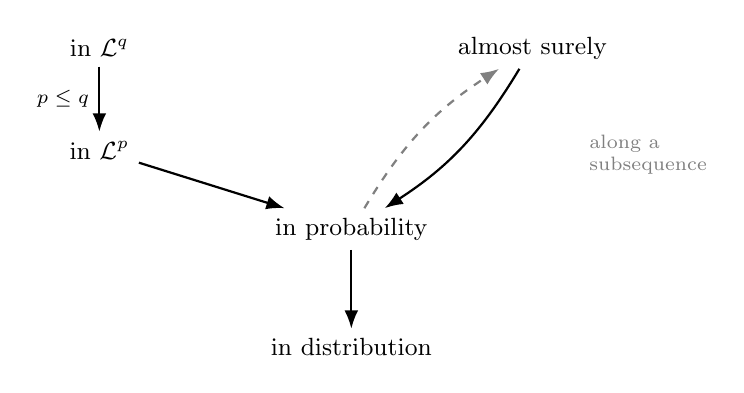
\begin{tikzpicture}[x=1cm, y=1cm, >=Latex, font=\small]
	\node (Lq) at (-3.2,2.3) {in $\cL^q$};
	\node (Lp) at (-3.2,1.0) {in $\cL^p$};
	\node (as) at (2.3,2.3) {almost surely};
	\node (pr) at (0,0) {in probability};
	\node (di) at (0,-1.5) {in distribution};
	\draw[->, thick] (Lq) -- node[left, font=\scriptsize] {$p \leq q$} (Lp);
	\draw[->, thick] (Lp) -- (pr);
	\draw[->, thick] (as) to[bend left=13] (pr);
	\draw[->, thick, dashed, gray] (pr) to[bend left=13] (as);
	\draw[->, thick] (pr) -- (di);
	\node[anchor=west, align=left, font=\scriptsize, gray] at (2.9,0.95) {along a\\ subsequence};
\end{tikzpicture}
\end{center}

\begin{example}[Counterexamples to the converses]\label{ex:mode-counter}
	Work on $\big((0,1),\cB,\mu\big)$ unless stated otherwise.
	\begin{enumerate}[label=(\roman*)]
		\item \emph{In probability but not in $\cL^1$.} Let $X_n = n\ind_{(0,1/n)}$. Then $\PP(|X_n|>\varepsilon)=1/n\to0$, but $\EE[X_n]=1$ for all $n$, so $X_n \not\to0$ in $\cL^1$. This is the escaping bump of Example \ref{pm-ex:bump} again.
		\item \emph{In probability but not almost surely.} Take the `typewriter sequence': for $n = 2^k + j$ with $0 \leq j < 2^k$, let $X_n = \ind_{(j2^{-k},(j+1)2^{-k})}$. Then $\PP(X_n \neq 0)=2^{-k}\to0$, so $X_n \xrightarrow{\PP}0$; but for every $\omega$ the sequence $X_n(\omega)$ takes the value $1$ infinitely often, so $X_n \not\to 0$ anywhere.
		\item \emph{In $\cL^1$ but not in $\cL^2$.} Let $X_n = n^{1/2}\ind_{(0,1/n)}$. Then $\|X_n\|_1 = n^{-1/2}\to0$ but $\|X_n\|_2^2 = 1$.
		\item \emph{In distribution but not in probability.} Let $X \sim N(0,1)$ and $X_n = -X$ for all $n$. Since $-X\sim N(0,1)$, we have $X_n \xrightarrow{d}X$; but $\PP(|X_n - X|>\varepsilon)=\PP(|2X|>\varepsilon)$ does not tend to zero.
		\item \emph{Almost surely but not in $\cL^1$.} The bump $X_n = n^2\ind_{(0,1/n)}$ converges to $0$ pointwise on $(0,1)$ but $\EE X_n = n \to\infty$.
	\end{enumerate}
\end{example}

The one useful partial converse is that convergence in distribution to a \emph{constant} implies convergence in probability: if $X_n \xrightarrow{d} c$ then $\PP(|X_n - c|>\varepsilon)\leq 1 - F_{X_n}(c+\varepsilon/2)+F_{X_n}(c-\varepsilon)\to 0$.

\subsection{Uniform integrability}

The examples above suggest the obstruction to upgrading convergence in probability to convergence in $\cL^1$ is exactly the escaping-mass phenomenon. Uniform integrability is the hypothesis that rules it out.

We start with a lemma showing that a single integrable random variable never has escaping mass.

\begin{lemma}\label{lem:ui-single}
	Let $X \in \cL^1(\PP)$. Then
	$$
	I_X(\delta) = \sup\big\{ \EE[|X|\ind_A] : A \in \cF, \; \PP(A)\leq\delta\big\} \longrightarrow 0 \quad \text{as } \delta \downarrow 0.
	$$
\end{lemma}
\begin{proof}
	$I_X$ is non-decreasing in $\delta$, so suppose for contradiction that $I_X(\delta) \geq \varepsilon$ for all $\delta>0$, for some $\varepsilon>0$. Then we may pick $A_n \in \cF$ with $\PP(A_n) \leq 2^{-n}$ and $\EE[|X|\ind_{A_n}]\geq\varepsilon$. Since $\sum_n\PP(A_n)<\infty$, the first Borel--Cantelli lemma gives $\PP(A)=0$ where $A = \limsup_n A_n$. Now $\ind_{\bigcup_{m\geq n}A_m}\downarrow \ind_A$, and $|X|\ind_{\bigcup_{m\geq n}A_m}\leq|X|\in\cL^1$, so by dominated convergence
	$$
	\varepsilon \leq \EE\big[|X|\ind_{A_n}\big] \leq \EE\Big[|X|\ind_{\bigcup_{m\geq n}A_m}\Big] \longrightarrow \EE[|X|\ind_A] = 0,
	$$
	a contradiction.
\end{proof}

\begin{definition}[Uniform integrability]
	A family $\cX \subseteq \cL^1(\PP)$ is \vocab{uniformly integrable} (UI) if it is bounded in $\cL^1$, i.e.\ $\sup_{X\in\cX}\EE|X|<\infty$, and
	$$
	I_\cX(\delta) = \sup\big\{ \EE[|X|\ind_A] : X \in \cX, \; \PP(A)\leq\delta\big\} \longrightarrow 0 \quad \text{as } \delta\downarrow 0.
	$$
\end{definition}

By Lemma \ref{lem:ui-single}, any finite family is UI. The following reformulation is usually the easiest to check.

\begin{lemma}[Equivalent form of UI]\label{lem:ui-equiv}
	A family $\cX\subseteq\cL^1(\PP)$ is uniformly integrable if and only if
	$$
	\sup_{X\in\cX}\EE\big[|X|\ind_{\{|X|>K\}}\big] \longrightarrow 0 \quad \text{as } K \to \infty.
	$$
\end{lemma}
\begin{proof}
	($\Rightarrow$) By Markov's inequality, $\PP(|X|>K)\leq \EE|X|/K \leq I_\cX(1)/K$ uniformly in $X\in\cX$. So given $\delta>0$ we may take $K$ large enough that $\PP(|X|>K)\leq\delta$ for all $X \in \cX$, and then $\EE[|X|\ind_{\{|X|>K\}}]\leq I_\cX(\delta)$, which tends to $0$.

	($\Leftarrow$) Fix $\varepsilon>0$ and choose $K$ with $\sup_{X}\EE[|X|\ind_{\{|X|>K\}}]<\varepsilon/2$. Then
	$$
	\EE|X| = \EE\big[|X|\ind_{\{|X|\leq K\}}\big]+\EE\big[|X|\ind_{\{|X|>K\}}\big] \leq K + \tfrac\varepsilon2,
	$$
	so $\cX$ is $\cL^1$-bounded. And for $A$ with $\PP(A)\leq\delta$,
	$$
	\EE[|X|\ind_A] \leq \EE\big[|X|\ind_A\ind_{\{|X|\leq K\}}\big]+\EE\big[|X|\ind_{\{|X|>K\}}\big] \leq K\delta+\tfrac\varepsilon2 < \varepsilon
	$$
	for $\delta < \varepsilon/(2K)$.
\end{proof}

\begin{example}[When UI holds and when it fails]
	\begin{enumerate}[label=(\roman*)]
		\item If $\cX$ is bounded in $\cL^p$ for some $p>1$ then it is UI: by H\"older with conjugate $q$,
		$$
		\EE[|X|\ind_A] \leq \|X\|_p \PP(A)^{1/q} \leq \big(\sup_X\|X\|_p\big)\delta^{1/q}\to0.
		$$
		\item If $|X| \leq Y$ for all $X \in \cX$ with $Y \in\cL^1$, then $\cX$ is UI, by Lemma \ref{lem:ui-single} applied to $Y$. So domination is a special case of uniform integrability.
		\item The family $\{n\ind_{(0,1/n)} : n\in\N\}$ on $(0,1)$ is bounded in $\cL^1$ (each has norm $1$) but not UI: taking $A = (0,1/n)$ gives $\PP(A)\to0$ while $\EE[X_n \ind_A]=1$.
	\end{enumerate}
\end{example}

\subsection{The Vitali convergence theorem}

We can now state the theorem which makes uniform integrability the right concept: it characterises $\cL^1$ convergence exactly. First a bounded case.

\begin{theorem}[Bounded convergence in probability]\label{thm:bdd-conv}
	Let $X_n\xrightarrow{\PP}X$ with $|X_n| \leq C < \infty$ almost surely for all $n$. Then $X_n \to X$ in $\cL^1$.
\end{theorem}
\begin{proof}
	Along a subsequence $X_{n_k}\to X$ a.s., so $|X|\leq C$ a.s. Given $\varepsilon>0$, split according to whether $|X_n - X|$ exceeds $\varepsilon/2$:
	$$
	\EE|X_n - X| = \EE\big[|X_n-X|\ind_{\{|X_n-X|>\varepsilon/2\}}\big]+\EE\big[|X_n-X|\ind_{\{|X_n-X|\leq\varepsilon/2\}}\big],
	$$
	$$
	\text{so} \qquad \EE|X_n-X| \leq 2C\,\PP\big(|X_n-X|>\tfrac\varepsilon2\big)+\tfrac\varepsilon2,
	$$
	which is $<\varepsilon$ for $n$ large.
\end{proof}

\begin{theorem}[Vitali convergence theorem]\label{thm:vitali}
	Let $X_n, X$ be random variables. The following are equivalent:
	\begin{enumerate}[label=(\roman*)]
		\item $X_n, X \in \cL^1(\PP)$ and $X_n \to X$ in $\cL^1$;
		\item $\{X_n : n \in\N\}$ is uniformly integrable and $X_n \xrightarrow{\PP} X$.
	\end{enumerate}
\end{theorem}
\begin{proof}
	(i)$\Rightarrow$(ii). Markov's inequality gives $\PP(|X_n-X|>\varepsilon)\leq \EE|X_n-X|/\varepsilon\to0$, so $X_n\xrightarrow{\PP}X$. For uniform integrability, fix $\varepsilon>0$ and take $N$ with $\EE|X_n - X|<\varepsilon/2$ for $n \geq N$. The finite family $\{X, X_1,\dots,X_N\}$ is UI by Lemma \ref{lem:ui-single}, so there is $\delta>0$ with $\EE[|Y|\ind_A]<\varepsilon/2$ for $Y$ in that family and $\PP(A)\leq\delta$. For $n>N$ and such $A$,
	$$
	\EE[|X_n|\ind_A] \leq \EE[|X_n - X|\ind_A]+\EE[|X|\ind_A] < \tfrac\varepsilon2+\tfrac\varepsilon2 = \varepsilon.
	$$
	So the whole family is UI.

	(ii)$\Rightarrow$(i). Along a subsequence $X_{n_k}\to X$ a.s., so by Fatou
	$$
	\EE|X| = \EE\big[\liminf_k |X_{n_k}|\big]\leq\liminf_k \EE|X_{n_k}|\leq \sup_n \EE|X_n|<\infty,
	$$
	so $X \in \cL^1$. Now let $g_K(x) = (-K)\vee x \wedge K$ be the truncation at level $K$; it is $1$-Lipschitz, so
	$$
	\PP\big(|g_K(X_n)-g_K(X)|>\varepsilon\big)\leq \PP(|X_n - X|>\varepsilon)\to0,
	$$
	and $|g_K(\cdot)|\leq K$, so by Theorem \ref{thm:bdd-conv} $g_K(X_n)\to g_K(X)$ in $\cL^1$. Therefore
	\begin{align*}
		\EE|X_n - X| &\leq \EE\big|X_n - g_K(X_n)\big| + \EE\big|g_K(X_n)-g_K(X)\big|+\EE\big|g_K(X)-X\big|\\
		&\leq \EE\big[|X_n|\ind_{\{|X_n|>K\}}\big]+\EE\big|g_K(X_n)-g_K(X)\big|+\EE\big[|X|\ind_{\{|X|>K\}}\big].
	\end{align*}
	Given $\varepsilon>0$, choose $K$ so that the first and third terms are each below $\varepsilon/3$ -- possible by Lemma \ref{lem:ui-equiv} for the first, and by Lemma \ref{lem:ui-single} for the third -- and then $n$ large so the middle term is below $\varepsilon/3$.
\end{proof}

\begin{remark}
	Vitali's theorem contains the dominated convergence theorem on a probability space as a special case: domination by an integrable $Y$ gives uniform integrability, and a.s.\ convergence gives convergence in probability. It is strictly stronger, since UI families need not be dominated.
\end{remark}

\section{Laws of Large Numbers}

The empirical content of probability theory is that averages of many independent measurements stabilise. We now prove this, in two forms of increasing strength.

\subsection{The weak law}

\begin{theorem}[Weak law of large numbers]\label{thm:wlln}
	Let $(X_n)$ be i.i.d.\ random variables with $\EE[X_1]=\nu$ and $\var(X_1)=\sigma^2<\infty$. Then
	$$
	\frac{1}{n}\sum_{i=1}^n X_i \xrightarrow{\;\PP\;} \nu \qquad \text{as } n \to\infty.
	$$
\end{theorem}
\begin{proof}
	Replacing $X_i$ by $X_i - \nu$ we may assume $\nu=0$. Let $S_n = \sum_{i\leq n}X_i$. By independence the variances add, so $\var(S_n) = n\sigma^2$, and Chebyshev's inequality gives
	$$
	\PP\Big( \Big|\frac{S_n}{n}\Big|>\varepsilon\Big) \leq \frac{\var(S_n)}{n^2\varepsilon^2}=\frac{\sigma^2}{n\varepsilon^2}\longrightarrow 0. \qedhere
	$$
\end{proof}

Notice that the proof also gives convergence in $\cL^2$, since $\EE[(S_n/n)^2]=\sigma^2/n\to0$. The theorem is `weak' in two respects: it assumes a second moment, and it concludes only convergence in probability. Both can be improved.

\subsection{A strong law under fourth moments}

Convergence in probability allows the averages to make large excursions infinitely often, provided they do so with vanishing probability -- the typewriter sequence of Example \ref{ex:mode-counter} does exactly that. The strong law rules this out. Here is a proof requiring a fourth moment, which is short and instructive; we will remove the hypothesis in \S10.

\begin{theorem}[Strong law under a fourth moment]\label{thm:slln4}
	Let $(X_n)$ be independent with $\EE[X_n]=\nu$ and $\EE[X_n^4]\leq M<\infty$ for all $n$. Then
	$$
	\frac{1}{n}\sum_{i=1}^n X_i \longrightarrow \nu \qquad \text{almost surely.}
	$$
\end{theorem}
\begin{proof}
	Replacing $X_n$ by $Y_n = X_n - \nu$, which satisfies $\EE[Y_n^4]\leq 2^4(\EE[X_n^4]+\nu^4)<\infty$ by convexity of $t \mapsto t^4$, we may assume $\nu=0$ and $\EE[X_n^4] \leq M$.

	Expand $\EE[S_n^4]$ where $S_n = \sum_{i\leq n}X_i$. A term $\EE[X_iX_jX_kX_\ell]$ with some index appearing exactly once vanishes by independence and $\EE[X_i]=0$; so the only surviving terms are those of the form $\EE[X_i^4]$ and $\EE[X_i^2X_j^2]$ with $i \neq j$. There are $n$ of the former and $\binom{n}{2}\binom{4}{2} = 3n(n-1)$ of the latter (choosing which two of the four factors carry index $i$), and by Cauchy--Schwarz $\EE[X_i^2X_j^2]\leq \sqrt{\EE X_i^4}\sqrt{\EE X_j^4}\leq M$. Hence
	$$
	\EE[S_n^4] \leq nM + 3n(n-1)M \leq 3n^2 M.
	$$
	Therefore, by Theorem \ref{thm:int-nonneg}(iv),
	$$
	\EE\Big[\sum_{n=1}^\infty \Big(\frac{S_n}{n}\Big)^4\Big] = \sum_{n=1}^\infty \frac{\EE[S_n^4]}{n^4} \leq \sum_{n=1}^\infty \frac{3M}{n^2}<\infty.
	$$
	A non-negative random variable with finite expectation is finite almost surely, so $\sum_n (S_n/n)^4 < \infty$ a.s., whence $(S_n/n)^4 \to 0$ and $S_n/n \to 0$ almost surely.
\end{proof}

\subsection{The strong law in general}

The theorem we are really after is the following, and it is the sharpest possible: no moment beyond the first is required, and the first cannot be dispensed with.

\begin{theorem}[Strong law of large numbers]\label{thm:slln}
	Let $(X_n)$ be i.i.d.\ with $\EE|X_1|<\infty$ and $\EE[X_1]=\nu$. Then
	$$
	\frac1n\sum_{i=1}^n X_i \longrightarrow \nu \qquad \text{almost surely, and in } \cL^1.
	$$
\end{theorem}

We will prove this in \S10 as a consequence of Birkhoff's ergodic theorem; the ergodic-theoretic route is the one taken in lectures and it is genuinely the cleanest. For now, observe that Kolmogorov's zero-one law already tells us something: the event $\{\frac1n\sum_{i\leq n}X_i \to c\}$ is a tail event, so it has probability $0$ or $1$, and $\limsup_n \frac1n\sum_{i\leq n}X_i$ is an almost surely constant element of $[-\infty,\infty]$. The strong law identifies that constant as $\EE[X_1]$.

\begin{remark}
	The integrability hypothesis cannot be weakened. If $\EE|X_1|=\infty$ then by the second Borel--Cantelli lemma applied to $A_n = \{|X_n|>n\}$ -- whose probabilities sum to $\infty$ precisely when $\EE|X_1|=\infty$ -- we get $|X_n|>n$ infinitely often almost surely, and hence $S_n/n$ cannot converge (since $\frac{X_n}{n} = \frac{S_n}{n}-\frac{n-1}{n}\frac{S_{n-1}}{n-1}$ would have to tend to zero). For a Cauchy sample, for instance, $S_n/n$ has the same Cauchy distribution for every $n$ and does not converge at all.
\end{remark}

\begin{remark}[How fast?]
	The strong law says $S_n/n \to \nu$; the central limit theorem of \S9 will say that the error is of order $n^{-1/2}$ in distribution. Sharper still, the \emph{law of the iterated logarithm} states that if $\EE X_1 = 0$ and $\var X_1 = 1$ then
	$$
	\limsup_n \frac{S_n}{\sqrt{2n\log\log n}} = 1, \qquad \liminf_n \frac{S_n}{\sqrt{2n\log\log n}}=-1 \qquad \text{a.s.}
	$$
	In particular $S_n/\sqrt n$ does \emph{not} converge almost surely -- it oscillates forever between $\pm\sqrt{2\log\log n}$ -- so the central limit theorem really is a statement about distributions and nothing more.
\end{remark}
\section{Fourier Transforms and Characteristic Functions}

\subsection{The Fourier transform in \texorpdfstring{$L^1$}{L1}}

We now allow complex-valued functions. For $f = u + iv$ with $u,v$ real and integrable, define $\int f = \int u + i\int v$; this is complex-linear, and the fundamental estimate still holds:

\begin{lemma}
	For $f \in L^1(\R^d;\C)$ we have $\big|\int f\big| \leq \int|f|$.
\end{lemma}
\begin{proof}
	Choose $\alpha \in \C$ with $|\alpha|=1$ and $\alpha\int f = |\int f|$. Then $\big|\int f\big| = \int \alpha f$ is real, so it equals $\int \re(\alpha f) \leq \int |\alpha f| = \int|f|$.
\end{proof}

Write $L^p(\R^d)$ for the complex $L^p$ spaces with respect to Lebesgue measure, and $\ip{u}{x}=\sum_i u_ix_i$.

\begin{definition}[Fourier transform]
	For $f \in L^1(\R^d)$ the \vocab{Fourier transform} is
	$$
	\hat f(u) = \int_{\R^d} f(x)e^{i\ip{u}{x}}\dd x, \qquad u \in \R^d.
	$$
	For a finite Borel measure $\mu$ on $\R^d$, set $\hat\mu(u)=\int_{\R^d}e^{i\ip{u}{x}}\dd\mu(x)$.
\end{definition}

\begin{remark}
	Immediately $|\hat f(u)| \leq \|f\|_1$ and $|\hat\mu(u)|\leq\mu(\R^d)$. Moreover if $u_n \to u$ then $e^{i\ip{u_n}{x}}\to e^{i\ip{u}{x}}$ pointwise, dominated by $|f|$ (respectively by $1$, integrable for a finite measure), so by dominated convergence $\hat f$ and $\hat\mu$ are \emph{continuous and bounded}. If $\mu$ has density $f$ then $\hat\mu = \hat f$.

	Different authors put the $2\pi$ and the sign in different places; the convention above is the one used in this course, and it is chosen so that the characteristic function below comes out with no constants at all.
\end{remark}

\begin{definition}[Characteristic function]
	Let $X$ be an $\R^d$-valued random variable with law $\mu_X$. Its \vocab{characteristic function} is
	$$
	\varphi_X(u) = \EE\big[e^{i\ip{u}{X}}\big] = \hat\mu_X(u).
	$$
\end{definition}

So $\varphi_X$ is continuous, $\varphi_X(0)=1$, $|\varphi_X(u)|\leq1$, and $\varphi_X(-u)=\overline{\varphi_X(u)}$. Our goals are: (a) $\varphi_X$ determines $\mu_X$; (b) pointwise convergence of $\varphi_{X_n}$ implies convergence in distribution of $X_n$; and (c) hence the central limit theorem. All three go through Gaussians.

\subsection{Convolution}

\begin{definition}[Convolution]
	Let $f \in L^1(\R^d)$ and let $\nu$ be a probability measure on $\R^d$. Define
	$$
	(f*\nu)(x) = \begin{cases}\int_{\R^d}f(x-y)\dd\nu(y), & \text{if } y\mapsto f(x-y) \in L^1(\nu),\\ 0,&\text{otherwise.}\end{cases}
	$$
	If $\nu$ has density $g$ we write $f * g$. For probability measures $\mu,\nu$ the convolution $\mu*\nu$ is the law of $X+Y$ with $X\sim\mu$, $Y\sim\nu$ independent, so
	$$
	(\mu*\nu)(A) = \int_{\R^d}\int_{\R^d}\ind_A(x+y)\dd\nu(y)\dd\mu(x).
	$$
\end{definition}

\begin{proposition}\label{prop:conv-contraction}
	For $1\leq p<\infty$ and $f \in L^p(\R^d)$, the map $f \mapsto f*\nu$ is a contraction of $L^p(\R^d)$: $\|f*\nu\|_p \leq \|f\|_p$. In particular $y \mapsto f(x-y)$ lies in $L^p(\nu)$ for almost every $x$.
\end{proposition}
\begin{proof}
	Since $\nu$ is a probability measure, Jensen's inequality applied to the convex function $t\mapsto |t|^p$ gives
	$$
	\Big| \int f(x-y)\dd\nu(y)\Big|^p \leq \int |f(x-y)|^p\dd\nu(y).
	$$
	Integrating in $x$ and applying Tonelli together with translation invariance of Lebesgue measure,
	$$
	\int_{\R^d}\int_{\R^d}|f(x-y)|^p\dd\nu(y)\dd x = \int_{\R^d}\Big(\int_{\R^d}|f(x-y)|^p\dd x\Big)\dd\nu(y) = \|f\|_p^p. \qedhere
	$$
\end{proof}

\begin{proposition}\label{prop:conv-fourier}
	$\widehat{f*\nu} = \hat f\,\hat\nu$ and $\widehat{\mu*\nu}=\hat\mu\,\hat\nu$. If $\mu$ has density $f$ then $\mu*\nu$ has density $f*\nu$.
\end{proposition}
\begin{proof}
	The second identity is a one-liner: with $X\sim\mu$, $Y\sim\nu$ independent,
	$$
	\widehat{\mu*\nu}(u) = \EE\big[e^{i\ip{u}{X+Y}}\big]=\EE\big[e^{i\ip{u}{X}}\big]\EE\big[e^{i\ip{u}{Y}}\big]=\hat\mu(u)\hat\nu(u),
	$$
	using Proposition \ref{prop:indep-product}(iii). The first follows by Fubini:
	$$
	\widehat{f*\nu}(u) = \int\!\!\int f(x-y)e^{i\ip{u}{x}}\dd\nu(y)\dd x = \int e^{i\ip{u}{y}}\Big(\int f(z)e^{i\ip{u}{z}}\dd z\Big)\dd\nu(y),
	$$
	which is $\hat f(u)\hat\nu(u)$, on substituting $z = x-y$. For the density claim, with $A$ Borel,
	$$
	(\mu*\nu)(A) = \int\!\!\int\ind_A(x+y)f(x)\dd x\dd\nu(y) = \int \ind_A(v)\Big(\int f(v-y)\dd\nu(y)\Big)\dd v. \qedhere
	$$
\end{proof}

In probabilistic language: the characteristic function of a sum of independent random variables is the product of their characteristic functions. That single fact is what makes characteristic functions the tool of choice for limit theorems about sums.

\subsection{Gaussians}

\begin{definition}
	For $t>0$ let $g_t$ denote the density of the $N(0,tI_d)$ distribution on $\R^d$:
	$$
	g_t(x) = (2\pi t)^{-d/2}e^{-|x|^2/(2t)}.
	$$
\end{definition}

\begin{proposition}\label{prop:gauss-ft}
	$\hat g_t(u) = e^{-|u|^2 t/2}$, and consequently $\hat g_t = (2\pi)^{d/2}t^{d/2}g_{1/t}$. The Fourier inversion formula
	$$
	g_t(x) = \frac{1}{(2\pi)^d}\int_{\R^d}e^{-i\ip{u}{x}}\hat g_t(u)\dd u
	$$
	holds for every $t>0$.
\end{proposition}
\begin{proof}
	Take $d=1$ and $t=1$ first, and let $\varphi(u)=\hat g_1(u)=\EE[e^{iuZ}]$ where $Z \sim N(0,1)$. Differentiating under the integral sign -- which is legitimate by Theorem \ref{thm:diff-under}, since $|\partial_u(e^{iux}g_1(x))| \leq |x|g_1(x)$ is integrable -- and then integrating by parts,
	$$
	\varphi'(u) = i\int_\R x e^{iux}g_1(x)\dd x = \frac{i}{\sqrt{2\pi}}\int_\R e^{iux}\Big(x e^{-x^2/2}\Big)\dd x,
	$$
	$$
	\varphi'(u) = \frac{i}{\sqrt{2\pi}}\Big[ -e^{iux}e^{-x^2/2}\Big]_{-\infty}^\infty + \frac{i^2 u}{\sqrt{2\pi}}\int_\R e^{iux}e^{-x^2/2}\dd x,
	$$
	so $\varphi'(u)=-u\varphi(u)$. Hence $\frac{d}{du}\big(e^{u^2/2}\varphi(u)\big)=0$, and since $\varphi(0)=1$ we get $\varphi(u)=e^{-u^2/2}$.

	In general, if $Z=(Z_1,\dots,Z_d)$ has i.i.d.\ $N(0,1)$ entries then $\sqrt t Z$ has density $g_t$, and by independence
	$$
	\hat g_t(u) = \EE\big[e^{i\ip{u}{\sqrt tZ}}\big] = \prod_{j=1}^d\EE\big[e^{iu_j\sqrt t Z_j}\big]=\prod_{j=1}^d e^{-u_j^2t/2}=e^{-|u|^2t/2}.
	$$
	Comparing with the definition of $g_{1/t}$ gives $\hat g_t = (2\pi)^{d/2}t^{d/2}g_{1/t}$. Applying the transform twice,
	$$
	\hat{\hat{g_t}} = (2\pi)^{d/2}t^{d/2}\hat g_{1/t} = (2\pi)^{d/2}t^{d/2}(2\pi)^{d/2}t^{-d/2}g_t = (2\pi)^d g_t,
	$$
	and since $g_t$ is even, $\hat{\hat{g_t}}(x) = \int e^{-i\ip{u}{x}}\hat g_t(u)\dd u$, which is the inversion formula.
\end{proof}

\begin{center}
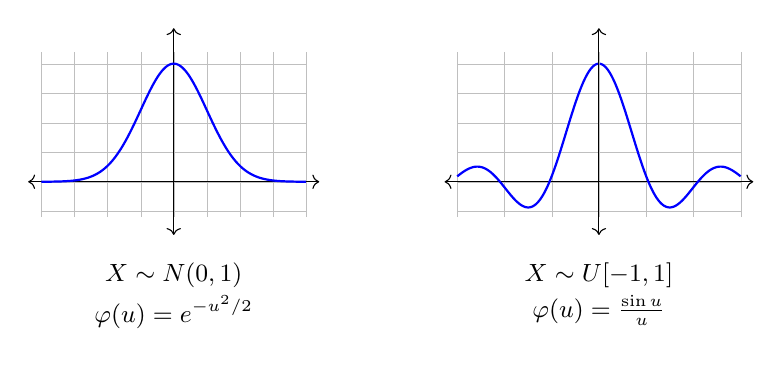
\begin{tikzpicture}
	\begin{scope}[x=0.42cm, y=1.5cm]
		\draw[ultra thin, color=lightgray] (-4,-0.3) grid[xstep=1, ystep=0.25] (4,1.1);
		\draw[<->] (-4.4,0) -- (4.4,0);
		\draw[<->] (0,-0.45) -- (0,1.3);
		\draw[thick, smooth, samples=140, domain=-4:4, color=blue] plot (\x, {exp(-\x*\x/2)});
		\node[font=\small, align=center, anchor=north] at (0,-0.6) {$X\sim N(0,1)$\\[2pt] $\varphi(u)=e^{-u^2/2}$};
	\end{scope}
	\begin{scope}[xshift=5.4cm]
	\begin{scope}[x=0.2cm, y=1.5cm]
		\draw[ultra thin, color=lightgray] (-9,-0.3) grid[xstep=3, ystep=0.25] (9,1.1);
		\draw[<->] (-9.8,0) -- (9.8,0);
		\draw[<->] (0,-0.45) -- (0,1.3);
		\draw[thick, smooth, samples=300, domain=-9:-0.05, color=blue] plot (\x, {sin(\x r)/(\x)});
		\draw[thick, smooth, samples=300, domain=0.05:9, color=blue] plot (\x, {sin(\x r)/(\x)});
		\node[font=\small, align=center, anchor=north] at (0,-0.6) {$X\sim U[-1,1]$\\[2pt] $\varphi(u)=\frac{\sin u}{u}$};
	\end{scope}
	\end{scope}
\end{tikzpicture}
\end{center}

\begin{definition}[Gaussian convolution]
	A \vocab{Gaussian convolution} is a function of the form $f * g_t$ with $f \in L^1(\R^d)$ and $t>0$.
\end{definition}

Gaussian convolutions are the technical device that makes everything work: they are smooth, their Fourier transforms decay rapidly, and they approximate arbitrary $L^p$ functions.

\begin{lemma}\label{lem:gauss-conv-inv}
	Fourier inversion holds for every Gaussian convolution:
	$$
	(f*g_t)(x) = \frac{1}{(2\pi)^d}\int_{\R^d}e^{-i\ip{u}{x}}\widehat{f*g_t}(u)\dd u = \frac{1}{(2\pi)^d}\int_{\R^d}e^{-i\ip{u}{x}}\hat f(u)e^{-|u|^2t/2}\dd u.
	$$
\end{lemma}
\begin{proof}
	Note first that $\widehat{f*g_t}(u)=\hat f(u)e^{-|u|^2t/2}$ is integrable, since $|\hat f|\leq\|f\|_1$. Now use inversion for $g_t$ and Fubini (justified since $(x,u)\mapsto f(x-y)\hat g_t(u)$ is absolutely integrable):
	\begin{align*}
		(2\pi)^d (f*g_t)(x) &= \int_{\R^d}f(x-y)\Big(\int_{\R^d}e^{-i\ip{u}{y}}\hat g_t(u)\dd u\Big)\dd y\\
		&= \int_{\R^d}e^{-i\ip{u}{x}}\Big(\int_{\R^d}f(x-y)e^{i\ip{u}{x-y}}\dd y\Big)\hat g_t(u)\dd u\\
		&= \int_{\R^d}e^{-i\ip{u}{x}}\hat f(u)\hat g_t(u)\dd u,
	\end{align*}
	substituting $z=x-y$ in the inner integral.
\end{proof}

\begin{lemma}[Gaussian convolutions approximate]\label{lem:gauss-dense}
	Let $1\leq p<\infty$ and $f \in L^p(\R^d)$. Then $\|f*g_t - f\|_p \to 0$ as $t \downarrow 0$.
\end{lemma}
\begin{proof}
	The space $C_c(\R^d)$ of continuous compactly supported functions is dense in $L^p(\R^d)$. Given $\varepsilon>0$ pick $h \in C_c$ with $\|f-h\|_p<\varepsilon/3$; by Proposition \ref{prop:conv-contraction},
	$$
	\|f*g_t - h*g_t\|_p = \|(f-h)*g_t\|_p \leq \|f-h\|_p<\varepsilon/3,
	$$
	so it suffices to prove the result for $h \in C_c(\R^d)$.

	Let $e(y)=\int_{\R^d}|h(x-y)-h(x)|^p\dd x$. Since $h$ is bounded with compact support, dominated convergence shows $e$ is continuous with $e(0)=0$, and $e(y) \leq 2^{p+1}\|h\|_p^p$ for all $y$. By Jensen as in Proposition \ref{prop:conv-contraction},
	\begin{align*}
		\|h*g_t - h\|_p^p &\leq \int_{\R^d}\!\int_{\R^d}|h(x-y)-h(x)|^p\dd x\,g_t(y)\dd y\\
		&=\int_{\R^d}\!e(y)g_t(y)\dd y = \int_{\R^d}\!e(\sqrt t z)g_1(z)\dd z,
	\end{align*}
	substituting $y = \sqrt t z$. As $t\downarrow0$ the integrand tends to $e(0)=0$ pointwise and is dominated by $2^{p+1}\|h\|_p^p g_1(z)$, so the integral tends to $0$.
\end{proof}

\subsection{Fourier inversion and Plancherel}

\begin{theorem}[Fourier inversion]\label{thm:fourier-inv}
	Let $f \in L^1(\R^d)$ with $\hat f \in L^1(\R^d)$. Then for almost every $x$,
	$$
	f(x) = \frac{1}{(2\pi)^d}\int_{\R^d}e^{-i\ip{u}{x}}\hat f(u)\dd u.
	$$
\end{theorem}
\begin{proof}
	By Lemma \ref{lem:gauss-conv-inv}, for every $t>0$,
	$$
	(f*g_t)(x)=\frac{1}{(2\pi)^d}\int_{\R^d}e^{-i\ip{u}{x}}\hat f(u)e^{-|u|^2t/2}\dd u.
	$$
	As $t \downarrow 0$ the right-hand side converges, for every $x$, to $\frac{1}{(2\pi)^d}\int e^{-i\ip{u}{x}}\hat f(u)\dd u$ by dominated convergence with dominating function $|\hat f| \in L^1$. On the left, Lemma \ref{lem:gauss-dense} gives $f*g_t \to f$ in $L^1$, hence in measure by Markov's inequality, hence almost everywhere along a subsequence $t_k \downarrow 0$. Uniqueness of limits gives the result almost everywhere.
\end{proof}

\begin{corollary}
	The Fourier transform is injective on $L^1(\R^d)$: if $\hat f = \hat g$ then $f = g$ almost everywhere.
\end{corollary}
\begin{proof}
	Apply the theorem to $f - g$, whose transform is $0 \in L^1$.
\end{proof}

\begin{theorem}[Plancherel identity]\label{pm-thm:plancherel}
	For $f \in L^1(\R^d)\cap L^2(\R^d)$ we have $\|\hat f\|_2 = (2\pi)^{d/2}\|f\|_2$.
\end{theorem}
\begin{proof}
	Suppose first that $\hat f \in L^1$ as well. Then $f$ and $\hat f$ are both bounded (being inverse transforms of $L^1$ functions) and integrable, so Fubini applies to $(x,u)\mapsto f(x)\hat f(u)$, and using inversion,
	\begin{align*}
		(2\pi)^d\|f\|_2^2 &= (2\pi)^d\int f(x)\overline{f(x)}\dd x = \int\Big(\int e^{-i\ip{u}{x}}\hat f(u)\dd u\Big)\overline{f(x)}\dd x\\
		&= \int \hat f(u)\overline{\Big(\int e^{i\ip{u}{x}}f(x)\dd x\Big)}\dd u = \int|\hat f(u)|^2\dd u = \|\hat f\|_2^2.
	\end{align*}
	For general $f \in L^1\cap L^2$, apply the above to $f_t = f * g_t$, whose transform $\hat f e^{-|u|^2t/2}$ is integrable. By Lemma \ref{lem:gauss-dense}, $\|f_t\|_2 \to \|f\|_2$; and $|\hat f(u)|^2e^{-|u|^2t}$ increases to $|\hat f(u)|^2$ as $t\downarrow0$, so $\|\hat f_t\|_2^2 \uparrow \|\hat f\|_2^2$ by monotone convergence. Passing to the limit in $(2\pi)^d\|f_t\|_2^2 = \|\hat f_t\|_2^2$ gives the result.
\end{proof}

\begin{corollary}[The Fourier transform on $L^2$]
	The map $F_0(f)=(2\pi)^{-d/2}\hat f$, defined on the dense subspace $L^1\cap L^2$ of $L^2(\R^d)$, extends uniquely to a linear isometry $F : L^2(\R^d)\to L^2(\R^d)$, the \vocab{Fourier--Plancherel transform}. It is in fact a surjective isometry, with $\ip{Ff}{Fg}=\ip{f}{g}$.
\end{corollary}
\begin{proof}
	$L^1 \cap L^2$ contains all $f\ind_{B(0,n)}$ for $f \in L^2$, hence is dense; $F_0$ is an isometry there by Theorem \ref{pm-thm:plancherel}; and $L^2$ is complete, so the extension exists and is unique. Preservation of the inner product follows by polarisation.
\end{proof}

\begin{example}
	Not every measure has an $L^1$ transform. For the Dirac mass $\delta_0$ on $\R$ we get $\hat\delta_0(u)=\int e^{iux}\dd\delta_0(x)=1$, which is not integrable, and indeed $\delta_0$ has no density. This is exactly the case the inversion theorem excludes.
\end{example}

\subsection{Characteristic functions determine laws}

\begin{theorem}[Uniqueness]\label{thm:cf-unique}
	Let $X$ be an $\R^d$-valued random variable. Then $\varphi_X$ determines $\mu_X$. If moreover $\varphi_X \in L^1(\R^d)$, then $\mu_X$ has a density given almost everywhere by
	$$
	f_X(x)=\frac{1}{(2\pi)^d}\int_{\R^d}e^{-i\ip{u}{x}}\varphi_X(u)\dd u.
	$$
\end{theorem}
\begin{proof}
	Let $Z$ be a standard Gaussian vector in $\R^d$ independent of $X$, so $\sqrt tZ$ has density $g_t$ and $X+\sqrt tZ$ has law $\mu_X * g_t$, which has density $f_t = \mu_X*g_t$. Since $\mu_X*g_t=(\mu_X*g_{t/2})*g_{t/2}$ and $\mu_X * g_{t/2}\in L^1$, this is a Gaussian convolution, so Lemma \ref{lem:gauss-conv-inv} gives
	$$
	f_t(x) = \frac{1}{(2\pi)^d}\int_{\R^d}e^{-i\ip{u}{x}}\varphi_X(u)e^{-|u|^2t/2}\dd u,
	$$
	which depends on $\mu_X$ only through $\varphi_X$.

	Now let $g : \R^d\to\R$ be bounded and continuous. Then $g(X+\sqrt tZ)\to g(X)$ almost surely as $t\downarrow0$, and $|g(X+\sqrt tZ)|\leq\|g\|_\infty$, so by bounded convergence
	$$
	\int_{\R^d}g(x)f_t(x)\dd x = \EE\big[g(X+\sqrt t Z)\big]\longrightarrow \EE[g(X)]=\int_{\R^d}g\dd\mu_X.
	$$
	The left-hand side is determined by $\varphi_X$, hence so is $\int g\dd\mu_X$ for every bounded continuous $g$; and two Borel probability measures agreeing against all such $g$ are equal. So $\varphi_X$ determines $\mu_X$.

	If $\varphi_X \in L^1$, dominated convergence shows $f_t(x)\to f_X(x)$ for every $x$, with $f_X$ as displayed, and $f_X \geq 0$ as a limit of the non-negative $f_t$. For $g$ bounded continuous with compact support, $|g(x)f_t(x)|\leq\|g\|_\infty(2\pi)^{-d}\|\varphi_X\|_1\ind_{\mathrm{supp}\,g}$, an integrable bound, so
	$$
	\int g f_X = \lim_{t\downarrow0}\int gf_t = \int g\dd\mu_X,
	$$
	whence $\mu_X$ has density $f_X$.
\end{proof}

\subsection{Weak convergence and L\'evy's continuity theorem}

\begin{definition}[Weak convergence]
	Borel probability measures $\mu_n$ on $\R^d$ \vocab{converge weakly} to $\mu$, written $\mu_n \weakto\mu$, if $\mu_n(g)\to\mu(g)$ for every bounded continuous $g : \R^d\to\R$. For random vectors we say $X_n \to X$ weakly if $\mu_{X_n}\weakto\mu_X$.
\end{definition}

\begin{remark}
	For $d=1$ weak convergence coincides with convergence in distribution as defined in \S7. (One direction: apply the definition to continuous approximations of $\ind_{(-\infty,x]}$ from above and below. The other uses the Skorokhod representation or a direct argument with the distribution functions.) It also suffices to test against $g \in C_c^\infty(\R^d)$, the smooth compactly supported functions, by a routine approximation.
\end{remark}

\begin{theorem}[L\'evy's continuity theorem]\label{thm:levy}
	Let $X_n, X$ be $\R^d$-valued random vectors with $\varphi_{X_n}(u)\to\varphi_X(u)$ for every $u \in\R^d$. Then $X_n \to X$ weakly.
\end{theorem}
\begin{proof}
	By the remark it suffices to show $\EE[g(X_n)]\to\EE[g(X)]$ for $g \in C_c^\infty(\R^d)$. Such a $g$ is bounded, integrable, and Lipschitz with some constant $\|g\|_{\mathrm{Lip}}$.

	Let $Z$ be a standard Gaussian vector independent of everything, and let $\varepsilon>0$. Choose $t>0$ small enough that $2\|g\|_{\mathrm{Lip}}\sqrt t\,\EE|Z| < 2\varepsilon/3$. Then
	\begin{align*}
		\big|\EE[g(X_n)]-\EE[g(X)]\big| &\leq \EE\big|g(X_n)-g(X_n+\sqrt tZ)\big| + \EE\big|g(X)-g(X+\sqrt tZ)\big|\\
		&\qquad + \big|\EE[g(X_n+\sqrt tZ)]-\EE[g(X+\sqrt tZ)]\big|\\
		&\leq \tfrac{2\varepsilon}{3}+\big|\EE[g(X_n+\sqrt tZ)]-\EE[g(X+\sqrt tZ)]\big|,
	\end{align*}
	using the Lipschitz bound on the first two terms. For the remaining term, write $f_{t,n}=\mu_{X_n}*g_t$ for the density of $X_n+\sqrt tZ$; by Lemma \ref{lem:gauss-conv-inv},
	$$
	\EE\big[g(X_n+\sqrt tZ)\big]=\int_{\R^d}\!g(x)f_{t,n}(x)\dd x = \frac{1}{(2\pi)^d}\int_{\R^d}\!\int_{\R^d}\!g(x)e^{-i\ip{u}{x}}\varphi_{X_n}(u)e^{-\frac{|u|^2t}{2}}\dd u\dd x.
	$$
	The integrand converges pointwise as $n \to\infty$ (since $\varphi_{X_n}\to\varphi_X$ pointwise) and is dominated by $|g(x)|e^{-|u|^2t/2}$, which is integrable on $\R^d\times\R^d$ because $|\varphi_{X_n}|\leq1$. So by dominated convergence the whole expression converges to $\EE[g(X+\sqrt tZ)]$, and the last term is below $\varepsilon/3$ for $n$ large.
\end{proof}

The converse is trivial: if $X_n \to X$ weakly, then testing against $x \mapsto \cos\ip{u}{x}$ and $x\mapsto\sin\ip{u}{x}$ gives $\varphi_{X_n}(u)\to\varphi_X(u)$. So convergence in distribution is \emph{equivalent} to pointwise convergence of characteristic functions, and this is what makes the following possible.

\subsection{The central limit theorem}

\begin{theorem}[Central limit theorem]\label{thm:clt}
	Let $(X_n)$ be i.i.d.\ real random variables with $\EE[X_1]=0$ and $\var(X_1)=1$, and let $S_n = \sum_{i=1}^n X_i$. Then
	$$
	\frac{S_n}{\sqrt n} \longrightarrow Z \sim N(0,1) \qquad \text{weakly, i.e.\ } \PP\Big(\frac{S_n}{\sqrt n}\leq x\Big)\to\PP(Z \leq x) \text{ for all } x \in \R.
	$$
\end{theorem}
\begin{proof}
	Let $\varphi = \varphi_{X_1}$. Since $\EE[X_1^2]<\infty$, Theorem \ref{thm:diff-under} lets us differentiate twice under the expectation:
	$$
	\varphi'(u)=i\EE\big[X_1e^{iuX_1}\big], \qquad \varphi''(u)=-\EE\big[X_1^2e^{iuX_1}\big],
	$$
	the dominating functions being $|X_1|$ and $X_1^2$. So $\varphi(0)=1$, $\varphi'(0)=i\EE[X_1]=0$ and $\varphi''(0)=-\EE[X_1^2]=-1$. Taylor's theorem with Peano remainder gives
	$$
	\varphi(v) = 1 - \frac{v^2}{2}+o(v^2) \qquad \text{as } v \to 0.
	$$
	Now by independence,
	$$
	\varphi_{S_n/\sqrt n}(u) = \EE\Big[e^{i\frac{u}{\sqrt n}(X_1+\cdots+X_n)}\Big]=\prod_{j=1}^n\EE\Big[e^{i\frac{u}{\sqrt n}X_j}\Big]=\Big[\varphi\Big(\frac{u}{\sqrt n}\Big)\Big]^n\! = \Big[1 - \frac{u^2}{2n}+o\Big(\frac1n\Big)\Big]^n\!\!.
	$$
	Fix $u$. For $n$ large the bracket is within a neighbourhood of $1$ where the principal branch of $\log$ satisfies $\log(1+z)=z+O(|z|^2)$, so
	$$
	\log \varphi_{S_n/\sqrt n}(u) = n\log\Big(1-\frac{u^2}{2n}+o(n^{-1})\Big) = n\Big(-\frac{u^2}{2n}+o(n^{-1})\Big)\longrightarrow -\frac{u^2}{2}.
	$$
	Hence $\varphi_{S_n/\sqrt n}(u)\to e^{-u^2/2}=\varphi_Z(u)$ for every $u$, and L\'evy's continuity theorem gives $S_n/\sqrt n \to Z$ weakly. Since the distribution function of $Z$ is continuous everywhere, the convergence holds at every $x$.
\end{proof}

\begin{remark}
	For general i.i.d.\ $X_i$ with mean $\nu$ and variance $\sigma^2 \in(0,\infty)$, apply the theorem to $(X_i-\nu)/\sigma$ to get
	$$
	\frac{S_n - n\nu}{\sigma\sqrt n}\longrightarrow N(0,1) \quad \text{weakly.}
	$$
	This is the version met in IA Probability, where it was proved for special cases using moment generating functions; the argument here is the general one, and the reason it works is that characteristic functions always exist whereas moment generating functions need not.
\end{remark}

\subsection{Gaussian random vectors}

\begin{definition}
	A random vector $X$ in $\R^d$ is a \vocab{Gaussian vector} if $\ip{X}{v}$ is a (possibly degenerate) real Gaussian random variable for every $v \in \R^d$.
\end{definition}

\begin{proposition}\label{prop:gaussian-vec}
	Let $X$ be a Gaussian vector in $\R^d$ with mean $m = \EE[X]$ and covariance matrix $V = (\cov(X_i,X_j))_{ij}$. Then:
	\begin{enumerate}[label=(\roman*)]
		\item $AX+b$ is a Gaussian vector in $\R^m$ for any $m\times d$ matrix $A$ and $b\in\R^m$;
		\item $\varphi_X(u)=\exp\big(i\ip{m}{u}-\tfrac12\ip{u}{Vu}\big)$, so $m$ and $V$ determine the law of $X$;
		\item if $V$ is invertible then $X$ has density
		$$
		f_X(x) = (2\pi)^{-d/2}(\det V)^{-1/2}\exp\Big(-\tfrac12\ip{x-m}{V^{-1}(x-m)}\Big);
		$$
		\item sub-vectors $X_{(1)}, X_{(2)}$ of $X$ are independent if and only if $\cov(X_{(1)},X_{(2)})=0$.
	\end{enumerate}
\end{proposition}
\begin{proof}[Proof sketch]
	(i) $\ip{AX+b}{v}=\ip{X}{A^Tv}+\ip{b}{v}$ is Gaussian.

	(ii) $\ip{u}{X}$ is real Gaussian with mean $\ip{m}{u}$ and variance $\ip{u}{Vu}$, and a real $N(\alpha,\sigma^2)$ variable $Y$ has $\EE[e^{iY}]=e^{i\alpha - \sigma^2/2}$ by Proposition \ref{prop:gauss-ft} and translation. Taking $\varphi_X(u)=\EE[e^{i\ip{u}{X}}]$ gives the formula, and Theorem \ref{thm:cf-unique} gives uniqueness.

	(iii) Write $V = \Sigma\Sigma^T$ and check that $m + \Sigma Z$, for $Z$ standard Gaussian, has the stated characteristic function; then change variables in the density of $Z$.

	(iv) If $\cov(X_{(1)},X_{(2)})=0$ then $V$ is block diagonal and $\varphi_X$ factorises as $\varphi_{X_{(1)}}\varphi_{X_{(2)}}$, so by uniqueness $\mu_X = \mu_{X_{(1)}}\otimes\mu_{X_{(2)}}$ and Proposition \ref{prop:indep-product} applies. The converse is immediate.
\end{proof}

Part (iv) deserves emphasis: for \emph{jointly} Gaussian variables, uncorrelated is the same as independent. This is false in general -- if $X\sim N(0,1)$ and $\epsilon = \pm1$ with equal probability independently of $X$, then $X$ and $\epsilon X$ are each standard Gaussian and uncorrelated, but obviously not independent; the pair $(X,\epsilon X)$ is not a Gaussian vector.

\begin{proposition}[Slutsky-type results]\label{prop:slutsky}
	Let $X_n \to X$ weakly in $\R^d$. Then
	\begin{enumerate}[label=(\roman*)]
		\item $h(X_n)\to h(X)$ weakly for any continuous $h : \R^d\to\R^k$;
		\item if $|X_n - Y_n|\to0$ in probability then $Y_n \to X$ weakly;
		\item if $Y_n \to c$ in probability for a constant $c$, then $(X_n,Y_n)\to(X,c)$ weakly.
	\end{enumerate}
	In particular $X_n + Y_n \to X+c$ weakly, and for $d=1$ also $X_nY_n \to cX$ weakly.
\end{proposition}
\begin{proof}
	(i) If $g$ is bounded continuous then so is $g\circ h$.

	(ii) It suffices to test against bounded Lipschitz $g$. Splitting on whether $|X_n - Y_n|$ exceeds $\eta = \varepsilon/(3\|g\|_{\mathrm{Lip}})$,
	$$
	\EE|g(X_n)-g(Y_n)| \leq \|g\|_{\mathrm{Lip}}\eta + 2\|g\|_\infty\PP(|X_n-Y_n|>\eta)<\tfrac{2\varepsilon}{3}
	$$
	for $n$ large, and $|\EE[g(X_n)]-\EE[g(X)]|<\varepsilon/3$ for $n$ large.

	(iii) $(X_n,c)\to(X,c)$ weakly, since $g(\cdot,c)$ is bounded continuous; and $|(X_n,Y_n)-(X_n,c)|=|Y_n-c|\to0$ in probability, so (ii) applies.
\end{proof}

These are the results one uses in statistics to justify replacing an unknown variance by a consistent estimator inside a central limit theorem.
\section{Ergodic Theory}

\subsection{Measure-preserving transformations}

Ergodic theory studies the long-run behaviour of a system evolving under repeated application of a single map. We will develop just enough of it to prove the strong law of large numbers in full generality, which turns out to be a special case.

Throughout, $(E,\cE,\mu)$ is a $\sigma$-finite measure space.

\begin{definition}[Measure-preserving]
	A measurable map $\Theta : E \to E$ is \vocab{measure-preserving} if $\mu(\Theta^{-1}(A))=\mu(A)$ for all $A \in \cE$.
\end{definition}

If $\Theta$ is measure-preserving then $\mu\circ\Theta^{-1}=\mu$, so by the change of variables formula (Proposition \ref{prop:change-var}), for any $f \in L^1(\mu)$ we have $f \circ \Theta \in L^1(\mu)$ with
$$
\int_E f\circ\Theta\dd\mu = \int_E f\dd\mu.
$$

\begin{definition}[Invariance and ergodicity]
	A set $A \in \cE$ is \vocab{invariant} if $\Theta^{-1}(A)=A$, and a measurable $f : E \to \R$ is invariant if $f\circ\Theta = f$. We write $\cE_\Theta$ for the collection of invariant sets.

	We say $\Theta$ is \vocab{ergodic} if every invariant $A$ satisfies $\mu(A)=0$ or $\mu(A^c)=0$.
\end{definition}

One checks at once that $\cE_\Theta$ is a $\sigma$-algebra, and that $f$ is invariant if and only if it is $\cE_\Theta$-measurable. Consequently, if $\Theta$ is ergodic then every invariant $f$ is almost everywhere constant: the sets $\{f \leq y\}$ are invariant, so $y \mapsto \mu(\{f\leq y\})$ takes only the values $0$ and $\mu(E)$, and $f$ equals $\inf\{y : \mu(f>y)=0\}$ a.e.

Ergodicity says that the system cannot be split into two non-trivial pieces which do not communicate. It is the dynamical analogue of irreducibility for a Markov chain.

\begin{example}[Circle rotation]\label{ex:rotation}
	Take $(E,\cE,\mu)=\big((0,1],\cB,\text{Lebesgue}\big)$ and, for $a \in (0,1)$,
	$$
	\Theta_a(x) = x + a \bmod 1.
	$$
	This preserves $\mu$ by the translation invariance established in \S2.5. It is ergodic if and only if $a$ is irrational. If $a = p/q$ is rational then $\Theta_a^q = \mathrm{id}$, so the union of $q$ well-separated small intervals spaced $1/q$ apart is invariant and non-trivial. If $a$ is irrational, the orbit $\{x, x\oplus a, x\oplus 2a,\dots\}$ of any point is dense in the circle, and this can be turned into a proof of ergodicity (one convenient route uses Fourier coefficients: if $f$ is invariant and in $L^2$ then its Fourier coefficients satisfy $\hat f(k)e^{2\pi i k a}=\hat f(k)$, forcing $\hat f(k)=0$ for $k \neq 0$).
\end{example}

\begin{center}
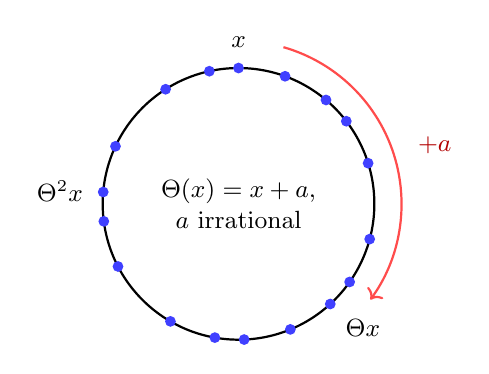
\begin{tikzpicture}[scale=1.5]
	\draw[thick] (0,0) circle (1.15);
	\foreach \k in {0,...,17}{
		\pgfmathsetmacro{\ang}{90 - 137.507*\k}
		\fill[blue!75] (\ang:1.15) circle (1.3pt);
	}
	% one arrow showing the rotation by a
	\draw[->, red!70, thick] (74:1.38) arc (74:-36:1.38);
	\node[red!70!black, font=\small, anchor=west] at (19:1.52) {$+a$};
	\node[font=\small, anchor=south] at (90:1.24) {$x$};
	\node[font=\small, anchor=north west] at (-47.5:1.22) {$\Theta x$};
	\node[font=\small, anchor=east] at (175:1.24) {$\Theta^2 x$};
	\node[font=\small, align=center] at (0,0) {$\Theta(x)=x+a$,\\ $a$ irrational};
\end{tikzpicture}
\end{center}

Our object of study is the sequence of \vocab{ergodic averages}. For measurable $f$ set
$$
S_0(f)=0, \qquad S_n(f) = f + f\circ\Theta + \cdots+f\circ\Theta^{n-1}.
$$
The question is what $S_n(f)/n$ does as $n \to \infty$: does the time average of $f$ along an orbit converge, and if so, to what?

\subsection{The maximal ergodic lemma}

Everything follows from the following deceptively simple inequality.

\begin{lemma}[Maximal ergodic lemma]\label{pm-lem:maximal}
	Let $\Theta$ be measure-preserving on $(E,\cE,\mu)$ and let $f \in L^1(\mu)$. Put $S^\star = \sup_{n\geq0}S_n(f)$. Then
	$$
	\int_{\{S^\star>0\}} f \dd\mu \geq 0.
	$$
\end{lemma}
\begin{proof}
	Put $S_n^\star = \max_{0\leq k\leq n}S_k$, so $S_n^\star \geq 0$ (as $S_0 = 0$) and $S_n^\star \uparrow S^\star$. For $0 \leq k \leq n$,
	$$
	S_{k+1} = f + S_k \circ\Theta \leq f + S_n^\star\circ\Theta.
	$$
	Let $A_n = \{S_n^\star>0\}$, so $A_n \uparrow \{S^\star>0\}$. On $A_n$ the maximum defining $S_n^\star$ is attained at some $k \geq 1$, so
	$$
	S_n^\star = \max_{1\leq k \leq n}S_k \leq \max_{0\leq k\leq n-1}\big(f + S_n^\star\circ\Theta\big) = f + S_n^\star\circ\Theta \quad \text{on } A_n.
	$$
	Integrating over $A_n$,
	$$
	\int_{A_n}S_n^\star\dd\mu \leq \int_{A_n}S_n^\star\circ\Theta\dd\mu + \int_{A_n}f\dd\mu.
	$$
	On $A_n^c$ we have $S_n^\star=0\leq S_n^\star\circ\Theta$, so adding $\int_{A_n^c}S_n^\star\dd\mu \leq \int_{A_n^c}S_n^\star\circ\Theta\dd\mu$ gives
	$$
	\int_E S_n^\star\dd\mu \leq \int_E S_n^\star\circ\Theta\dd\mu+\int_{A_n}f\dd\mu = \int_E S_n^\star\dd\mu + \int_{A_n}f\dd\mu,
	$$
	using that $\Theta$ preserves $\mu$. As $S_n^\star$ is integrable (being bounded by $\sum_{k<n}|f|\circ\Theta^k$), we may cancel and obtain $\int_{A_n}f\dd\mu \geq 0$. Finally $f\ind_{A_n}\to f\ind_{\{S^\star>0\}}$ pointwise with $|f\ind_{A_n}|\leq|f| \in L^1$, so dominated convergence gives the claim.
\end{proof}

\subsection{Birkhoff's ergodic theorem}

\begin{theorem}[Birkhoff]\label{thm:birkhoff}
	Let $\Theta$ be measure-preserving on the $\sigma$-finite space $(E,\cE,\mu)$ and let $f \in L^1(\mu)$. Then there is an invariant $\bar f \in L^1(\mu)$ with $\mu(|\bar f|)\leq\mu(|f|)$ and
	$$
	\frac{S_n(f)}{n}\longrightarrow\bar f \qquad \text{almost everywhere.}
	$$
	If $\Theta$ is ergodic and $\mu$ is a probability measure, then $\bar f = \mu(f)$ almost everywhere.
\end{theorem}
\begin{proof}[Proof (non-examinable)]
	Observe that
	$$
	\limsup_n \frac{S_n(f)}{n} = \limsup_n \frac{S_n(f)\circ\Theta}{n},
	$$
	since $S_{n+1}(f) = f + S_n(f)\circ\Theta$ and $f/n \to 0$; similarly for $\liminf$. So both $\limsup_n S_n/n$ and $\liminf_n S_n/n$ are invariant functions, hence $\cE_\Theta$-measurable. For $a<b$ put
	$$
	D = D_{a,b}=\Big\{\liminf_n \frac{S_n(f)}{n}<a<b<\limsup_n\frac{S_n(f)}{n}\Big\},
	$$
	a measurable invariant set. We show $\mu(D)=0$.

	Assume without loss of generality $b>0$ (otherwise replace $f$ by $-f$ and swap the roles of $a$ and $b$). Let $B \subseteq D$ be measurable with $\mu(B)<\infty$, and put $g = f - b\ind_B \in L^1(\mu)$. Then
	$$
	S_n(g) = S_n(f)-bS_n(\ind_B) \geq S_n(f)-bn,
	$$
	which is positive for some $n$ at every point of $D$, by the definition of $\limsup$. Restrict the measure space to $D$: since $D$ is invariant, $\Theta$ is still measure-preserving for $\mu|_D$, because
	$$
	\mu|_D(\Theta^{-1}A)=\mu(\Theta^{-1}A \cap D) = \mu\big(\Theta^{-1}(A\cap D)\big)=\mu(A\cap D)=\mu|_D(A).
	$$
	On this restricted space $\{S^\star(g)>0\}=D$, so the maximal ergodic lemma gives
	$$
	0 \leq \int_D g\dd\mu = \int_D f\dd\mu - b\mu(B),
	$$
	that is, $b\mu(B)\leq \int_D f\dd\mu$. By $\sigma$-finiteness we may choose $B_n \uparrow D$ with $\mu(B_n)<\infty$ and let $n \to\infty$, obtaining $b\mu(D)\leq\int_Df\dd\mu$. Running the same argument with $-f$ and $-a$ in place of $f$ and $b$ gives $-a\mu(D)\leq -\int_Df\dd\mu$, so
	$$
	b\mu(D)\leq\int_D f\dd\mu\leq a\mu(D).
	$$
	Since $a<b$ this forces $\mu(D)=0$ or $\mu(D)=\infty$; but $\int_D f\dd\mu$ is finite, so $\mu(D)=0$.

	Now let
	$$
	\Delta = \Big\{\liminf_n\frac{S_n(f)}{n}<\limsup_n\frac{S_n(f)}{n}\Big\}=\bigcup_{a<b,\; a,b\in\Q}D_{a,b},
	$$
	a countable union of null sets, so $\mu(\Delta)=0$. Off $\Delta$ the limit $\lim_n S_n(f)/n$ exists in $[-\infty,\infty]$; define $\bar f$ to be that limit on $\Delta^c$ and $0$ on $\Delta$. Then $\bar f$ is invariant and $S_n(f)/n\to\bar f$ almost everywhere.

	Finally, since $\Theta$ is measure-preserving, $\mu(|f\circ\Theta^k|)=\mu(|f|)$, so $\mu(|S_n(f)|)\leq n\mu(|f|)$, and by Fatou
	$$
	\mu(|\bar f|)=\mu\Big(\liminf_n\Big|\frac{S_n(f)}{n}\Big|\Big)\leq\liminf_n\mu\Big(\Big|\frac{S_n(f)}{n}\Big|\Big)\leq\mu(|f|)<\infty.
	$$
	In particular $\bar f$ is finite almost everywhere. If $\Theta$ is ergodic then $\bar f$ is a.e.\ constant; if additionally $\mu(E)=1$, the von Neumann theorem below identifies the constant as $\mu(f)$.
\end{proof}

\subsection{Von Neumann's \texorpdfstring{$L^p$}{Lp} ergodic theorem}

\begin{theorem}[von Neumann]\label{thm:vonneumann}
	Let $(E,\cE,\mu)$ be a \emph{finite} measure space, $\Theta$ measure-preserving, and $1 \leq p<\infty$. Then for $f \in L^p(\mu)$,
	$$
	\frac{S_n(f)}{n}\longrightarrow\bar f \qquad \text{in } L^p(\mu),
	$$
	where $\bar f$ is the almost-everywhere limit from Birkhoff's theorem.
\end{theorem}
\begin{proof}
	Since $\Theta$ preserves $\mu$, $\|f\circ\Theta^i\|_p = \|f\|_p$, so by Minkowski
	\begin{equation}\label{eq:contraction}
		\Big\|\frac{S_n(f)}{n}\Big\|_p \leq \frac1n\sum_{i=0}^{n-1}\|f\circ\Theta^i\|_p = \|f\|_p. \tag{$\sharp$}
	\end{equation}
	So $f \mapsto S_n(f)/n$ is a contraction of $L^p$, uniformly in $n$; this is the key.

	Fix $\varepsilon>0$. For $K>0$ let $f_K = (-K)\vee f\wedge K$. Then
	$$
	\|f-f_K\|_p^p = \int_E |f-f_K|^p\ind_{\{|f|>K\}}\dd\mu \longrightarrow 0
	$$
	as $K \to\infty$ by dominated convergence (the integrand is at most $2^p|f|^p \in L^1$ and tends to $0$ pointwise). Choose $K$ with $\|f-f_K\|_p<\varepsilon/3$.

	Since $\mu$ is finite we have $f_K \in L^1(\mu)$, so Birkhoff gives $S_n(f_K)/n \to \bar f_K$ almost everywhere, and $|S_n(f_K)/n|\leq K$, so that $|\bar f_K|\leq K$. By bounded convergence (Theorem \ref{pm-thm:dct}, with dominating constant $2K$, integrable as $\mu(E)<\infty$),
	$$
	\Big\|\frac{S_n(f_K)}{n}-\bar f_K\Big\|_p^p \leq (2K)^{p-1}\Big\|\frac{S_n(f_K)}{n}-\bar f_K\Big\|_1 \longrightarrow 0,
	$$
	so this term is below $(\varepsilon/3)^p$ for $n$ large.

	Also $f \in L^p(\mu)\subseteq L^1(\mu)$ since $\mu$ is finite, so Birkhoff applies to $f$ too and $S_n(f)/n \to \bar f$ a.e. By Fatou and the contraction property \eqref{eq:contraction},
	\begin{align*}
		\|\bar f - \bar f_K\|_p^p &= \int_E \liminf_n \Big|\frac{S_n(f-f_K)}{n}\Big|^p\dd\mu \leq \liminf_n \Big\|\frac{S_n(f-f_K)}{n}\Big\|_p^p\\
		&\leq \|f-f_K\|_p^p<(\varepsilon/3)^p.
	\end{align*}
	In particular $\bar f \in L^p$. Combining the three estimates via the triangle inequality,
	$$
	\Big\|\frac{S_n(f)}{n}-\bar f\Big\|_p \leq \Big\|\frac{S_n(f-f_K)}{n}\Big\|_p + \Big\|\frac{S_n(f_K)}{n}-\bar f_K\Big\|_p+\|\bar f_K-\bar f\|_p<\varepsilon
	$$
	for $n$ large.
\end{proof}

\begin{corollary}\label{cor:mean-identified}
	If $\mu$ is a probability measure and $\Theta$ is ergodic then, for $f \in L^1(\mu)$, $\bar f = \mu(f)$ almost everywhere.
\end{corollary}
\begin{proof}
	Ergodicity makes the invariant function $\bar f$ a.e.\ constant, say $\bar f = c$. By von Neumann with $p=1$, $\mu(S_n(f)/n)\to\mu(\bar f)=c$; but $\mu(S_n(f)/n)=\frac1n\sum_{k<n}\mu(f\circ\Theta^k)=\mu(f)$ for every $n$. So $c = \mu(f)$.
\end{proof}

\subsection{Bernoulli shifts}

To apply the ergodic theorems to i.i.d.\ sequences we need the right dynamical system. Let $E = \R^\N$, the space of real sequences $x = (x_n)$, and let
$$
\cC = \Big\{ \prod_{n=1}^\infty A_n : A_n \in \cB, \; A_n = \R \text{ for all large } n \Big\}
$$
be the collection of \vocab{cylinder sets}, a $\pi$-system. Put $\cE = \sigma(\cC)$, the \vocab{cylindrical $\sigma$-algebra}; it coincides with $\sigma(\{f_n : n \in \N\})$ where $f_n(x)=x_n$ are the coordinate maps, and with $\cB(\R^\N)$ for the product topology.

Let $m$ be a probability measure on $\R$, and let $(X_n)$ be i.i.d.\ with law $m$ -- these exist by Theorem \ref{thm:construct-iid}. Define $X : \Omega \to E$ by $X(\omega)=(X_1(\omega),X_2(\omega),\dots)$. This is $\cF$-$\cE$ measurable, since for a cylinder set $A$,
$$
X^{-1}(A) = \bigcap_{n=1}^N X_n^{-1}(A_n) \in \cF.
$$
Let $\mu = \PP\circ X^{-1}$. On cylinder sets,
$$
\mu\Big(\prod_{n=1}^\infty A_n\Big) = \lim_{N\to\infty}\PP(X_1 \in A_1,\dots,X_N \in A_N) = \prod_{n=1}^\infty m(A_n)
$$
(the product being eventually $1$). By uniqueness of extension, $\mu$ is the unique probability measure on $(E,\cE)$ with this property; we write $\mu = m^{\otimes\N}$ and call $(E,\cE,\mu)$ the \vocab{canonical model} for an i.i.d.\ sequence of law $m$.

\begin{definition}
	The \vocab{shift map} $\Theta : E \to E$ is $\Theta(x_1,x_2,x_3,\dots)=(x_2,x_3,x_4,\dots)$.
\end{definition}

\begin{theorem}\label{thm:shift-ergodic}
	The shift map $\Theta$ is measure-preserving and ergodic on $(E,\cE,\mu)$.
\end{theorem}
\begin{proof}
	For a cylinder set $A = \prod_n A_n$ with $A_n = \R$ for $n>N$,
	$$
	\mu(\Theta^{-1}A)=\PP(X_2\in A_1,\dots,X_{N+1}\in A_N)=\prod_{n=1}^N m(A_n)=\mu(A),
	$$
	using that the $X_i$ are i.i.d. As the cylinder sets form a $\pi$-system generating $\cE$ and both $\mu$ and $\mu\circ\Theta^{-1}$ are probability measures, uniqueness of extension gives $\mu\circ\Theta^{-1}=\mu$.

	For ergodicity, recall the tail $\sigma$-algebra $\cT = \bigcap_n \cT_n$ with $\cT_n = \sigma(f_k : k>n)$. For a cylinder set $A$,
	$$
	\Theta^{-n}(A) = \{x : (x_{n+1},x_{n+2},\dots)\in A\} \in \cT_n,
	$$
	and since $\{A : \Theta^{-n}(A)\in\cT_n\}$ is a $\sigma$-algebra containing $\cC$, this holds for all $A \in \cE$. So if $A$ is invariant then $A = \Theta^{-n}(A)\in\cT_n$ for every $n$, whence $A \in \cT$. By Kolmogorov's zero-one law (Theorem \ref{thm:kolmogorov01}), applied to the independent coordinate variables under $\mu$, we get $\mu(A)\in\{0,1\}$.
\end{proof}

\subsection{The strong law of large numbers}

We can now finish the job.

\begin{theorem}\label{thm:slln-canonical}
	Let $m$ be a probability measure on $\R$ with $\int_\R|x|\dd m(x)<\infty$ and $\int_\R x\dd m(x)=\nu$. Then, on the canonical model $(E,\cE,\mu)=(\R^\N,\sigma(\cC),m^{\otimes\N})$,
	$$
	\mu\Big(\Big\{ x \in \R^\N : \frac{x_1+\cdots+x_n}{n}\to\nu\Big\}\Big)=1.
	$$
\end{theorem}
\begin{proof}
	Take $f(x)=x_1$, the first coordinate map. Then by the change of variables formula,
	$$
	\int_E |f|\dd\mu = \int_\R |x|\dd m(x)<\infty,
	$$
	so $f \in L^1(\mu)$, and $\mu(f)=\nu$. Moreover
	$$
	S_n(f)(x)= f(x)+f(\Theta x)+\cdots+f(\Theta^{n-1}x)=x_1+x_2+\cdots+x_n.
	$$
	By Theorem \ref{thm:shift-ergodic} the shift is measure-preserving and ergodic, so Birkhoff's theorem gives $S_n(f)/n\to\bar f$ almost everywhere, and Corollary \ref{cor:mean-identified} identifies $\bar f = \mu(f)=\nu$.
\end{proof}

\begin{proof}[Proof of Theorem \ref{thm:slln}]
	Let $(X_n)$ be i.i.d.\ on $(\Omega,\cF,\PP)$ with $\EE|X_1|<\infty$ and common law $m$, and let $X : \Omega \to \R^\N$ be the associated map, so $\PP\circ X^{-1}=\mu$. Then
	$$
	\PP\Big(\frac1n\sum_{i=1}^nX_i \to \EE[X_1]\Big) = \mu\Big(\Big\{x : \frac{x_1+\cdots+x_n}{n}\to\nu\Big\}\Big)=1
	$$
	by Theorem \ref{thm:slln-canonical}, since the event on the left is the $X$-preimage of the event on the right. Convergence in $\cL^1$ follows from von Neumann's theorem with $p=1$ applied to the same $f$.
\end{proof}

\begin{remark}
	It is worth appreciating what has happened. The strong law is a statement about i.i.d.\ sequences, and its proof consisted of: (a) realising the sequence as a point of a single measure space $\R^\N$; (b) noticing that `shift the sequence along by one' is a measure-preserving ergodic transformation of that space; and (c) applying a completely general theorem about time averages. The independence enters only through Kolmogorov's zero-one law in step (b). Birkhoff's theorem is much more general than the strong law -- it applies to stationary sequences that are far from independent -- and this is why ergodic theory has become a subject in its own right.
\end{remark}

\begin{example}[Normal numbers]
	Take $m$ uniform on $\{0,1,\dots,9\}$, so that $(X_n)$ are the digits of a uniformly random real in $[0,1)$. Applying the strong law to $\ind_{\{X_n = k\}}$ gives that, almost surely, the digit $k$ has asymptotic frequency $1/10$ in the decimal expansion, for each $k$. Since a countable intersection of almost sure events is almost sure, Lebesgue-almost every real number is \vocab{normal} to base $10$. Exhibiting one explicitly is another matter entirely.
\end{example}

\section{Closing Remarks}

It is worth stepping back to see the shape of what we have built.

We began with the problem of assigning a size to subsets of a space, and found that we could not do it for all of them -- Carath\'eodory's theorem told us how far we could get, Dynkin's lemma told us that the answer was unique, and Vitali told us that we could not do better. From there, the class of measurable functions and the Lebesgue integral came almost for free, and the payoff was immediate: the monotone convergence theorem, Fatou's lemma and the dominated convergence theorem give us exactly the licence to exchange limits and integrals that the Riemann theory withheld. Fubini's theorem let us integrate in product spaces, which is to say, handle several random variables at once.

The second half was the harvest. The $L^p$ spaces gave us a complete normed setting for analysis, with $L^2$ a Hilbert space in which conditional expectation is nothing more exotic than orthogonal projection. Uniform integrability isolated exactly the hypothesis under which convergence in probability upgrades to convergence in $L^1$. Characteristic functions turned convolution into multiplication and thereby turned the central limit theorem into a Taylor expansion. And ergodic theory turned the strong law of large numbers into a statement about a shift map on sequence space.

Two threads run through all of it. The first is the $\pi$-system argument: almost every uniqueness statement we proved -- uniqueness of Lebesgue measure, of product measures, of the law determined by a distribution function or a characteristic function, of conditional expectation -- came from Dynkin's lemma or its functional cousin the monotone class theorem. The second is approximation from below: simple functions approximate non-negative measurable functions, and every theorem about the integral was proved first for indicators, then simple functions, then by monotone convergence in general. If you remember nothing else from this course, remember those two techniques; between them they prove most of it.

\end{document}
